%% ====================================================================%%
%%	Sample Driver file for use with uwthesis.sty
%% 	To print this document in the Math Dept, 
%%	do the following:
%%  		latex main
%%		bibtex main
%%		latex main (you may have to do this twice at this point)
%%		dvipr main
%%	To run this sa mple, you will also need the following files
%%		abs.tex, ack.tex,
%%		chap1.tex, chap2.tex, appendix.tex	
%%		thesis.bib	
%% ====================================================================%%
%% 
\documentclass[11pt]{report}

%% If you want to  process the graphics examples in Chap 3 uncomment this line
\usepackage{graphicx}
%\usepackage[sorting=none,firstinits=true,url=false,doi=true]{biblatex}
%\bibliography{/Users/warrick/Documents/MMB_Lab/Papers_and_Chapters/References/ReferenceLibrary}
\usepackage[square, numbers, sort&compress]{natbib}

\usepackage{StyleFiles/mythesis,StyleFiles/tgrind}
\usepackage{fancyhdr}
%% Use this if you only want to do Chap 1 things - basic stuff
%% NOTE: the uwthesis style file should go AFTER all the other packages
%% You may have conflicts if you call the amsthm.sty package after uwthesis.sty

\usepackage{amssymb,StyleFiles/uwthesis}

\graphicspath{
{./Chapters/Introduction/Figures/}
{./Chapters/Physics/Figures/}
{./Chapters/FluxCapacitor/Figures/}
{./Chapters/Concentrator/Figures/}
{./Chapters/Oscillator/Figures/}
{./Chapters/TumorCellAdhesion/Figures/}
{./Chapters/Cardiac/Figures/}
{./Chapters/RealTimeCM/Figures/}
{./Chapters/FutureDirections/Figures/}
{./Appendicies/DropletGeometry/Figures/}
{./Appendicies/Diffusion/Figures/}
{./Appendicies/Concentrator/Figures/}
{./Appendicies/Oscillator/Figures/}
{./Appendicies/DiffusionValve/Figures/}
{./Appendicies/Cardiac/Figures/}
{./Appendicies/RealTimeCM/Figures/}
}

\begin{document}

\title{Microscale Principles and Tools for Studying Cellular Interactions}
\author{Jay W. Warrick}

%\inputpicturetrue  % By Jeff McGough. See uuguide and private thesis.sty
%\inputpicturefalse % To NOT produce pictures, uncomment this line


\degree{Doctor of Philosophy}
\dept{Biomedical Engineering}
\thesistype{dissertation}
%% Starts page numbering as i, ii, etc.
\beforepreface
\prefacesection{Abstract}
\input frontmatter/abs 
\prefacesection{Acknowledgements}
\input frontmatter/ack 
\prefacesection{Papers}
\input frontmatter/papers
\listoffigures
\listoftables

\afterpreface

%% Include the Chapters
\chapter{Chapter 1: Introduction}\label{Chap:Introduction}





\section{Preface}
Microfluidics are super useful, wow did you know that? I mean they really are the coolest! You can do some really cool stuff with microfluidics when you take off the lid and do open microfluidics. I'm super serious. It's really great. You can do stuff like make Legos or you could do some other stuff like culture cells and do tissue culture in ways that you never thought of before.

\section{Microfluidics for Tissue culture}
Let's talk about tissue culture platforms that used microfluidics because those are really important  n


\section{}
Wow Teddy, you're so smart\cite{Vogler2004a}.





\chapter{Physics: Scaling Cell-Based Assays} % Write in your own chapter title
\label{Chap:Physics}
\begin{figure}[!b]
\centering
\begin{tabular}{c}
$t = 0.0\,$s 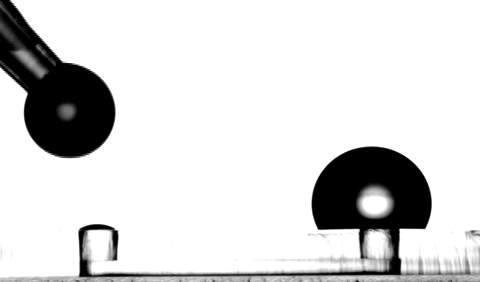
\includegraphics[width=2in]{PP_1.png} \cr
$t = 0.4\,$s 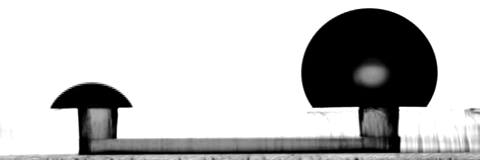
\includegraphics[width=2in]{PP_2.png} \cr
$t = 4.0\,$s 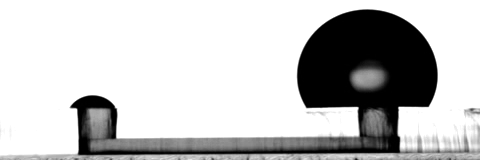
\includegraphics[width=2in]{PP_3.png} \cr
\end{tabular}
\caption{\textbf{Passive-pumping}. Images represent a time series originally taken by movie by Keil Regehr observing passive pumping using a Goniometer, an instrument for measuring the profiles of interfaces. Some frames of the movie are included here to illustrate fluid pumping in a microchannel using a manual pipette. In accordance with the Young-Laplace equation for the internal pressure of a droplet, the small droplet pumps towards the large droplet. The majority of the pumping occurs in less than a second while the remainder occurs as the wetted perimeter of the input droplet settles to a final diameter. Typically, the port radius or the protein adsorbed region surrounding the port defines the wetted perimeter, essentially eliminating the last phase equilibration of the wetted perimeter as compared to these images.}
\label{chap1:fig:passivePumping}
\end{figure}
This chapter summarizes efforts to characterize some basic advantages and challenges for micro-scale approaches to cell culture. Challenges include microchannel washing and evaporation while potential advantages include reduced volumes and control of diffusive transport. However, a brief mention of passive-pumping is necessary to put the following studies into context and is a terrific example of how a reduction in scale can affect the balance of physical forces, leading to new approaches for cell-based assays. 

As the volumes of fluids used for cell-based assays are reduced, the influence of gravity on the shape and flow of those fluids is reduced relative to surface tension. The Young-Laplace equation defines the pressure within a droplet with a curvature of radius, $R$, in a system with a surface tension constant of $\gamma$ (Eq \ref{chap1:equ:youngLaplace}). Passive-pumping has been thoroughly characterized by previous lab members \cite{Berthier:2007mi,Walker:2002ez}; however, an extensive appendix of equations used to model droplet geometries, pressures, volumes, and heights is provided to avoid others having to repeat this effort (Appendix \ref{App:DropletGeometry}).

\begin{equation}
\Delta P = \frac{\gamma}{2 R}
\label{chap1:equ:youngLaplace}
\end{equation}

%%%%%%%%%%%%%%%%%%%%%%
%%%%%%%%%%%%%%%%%%%%%%
%%%%%        Laminar Flow     %%%%%%%
%%%%%%%%%%%%%%%%%%%%%%

\section{Laminar Flow: Channel Washing and Treatments}
\paragraph{Preface.}The information in this section is adapted or summarized from \cite{Warrick:2007lq}.\\
\\
\noindent One of the first questions that is typically asked by a new user of microchannels is, ``How much fluid should I use to wash out the microchannel?'' The question is an important one for cell-based assays and is challenging given the parabolic flow profile characteristic of low Reynolds number flow (Fig \ref{chap1:fig:washing}A). At the boundary of the channels, the velocity of the fluid is zero, thus resulting in fluid left behind during washing. Fluorescent beads and food coloring were used to characterize the ability to remove this boundary layer via passive-pumping. Experimental results agree with an analytical model of laminar flow that predicts \% washing of the channel, $\Phi$, given the volume of the channel, $V_{channel}$, and the volume of the fluid used to wash the channel, $V_{wash}$ (Eq \ref{chap1:equ:washing}) \cite{Warrick:2007lq}. 
\begin{equation}
\Phi = 1 - \zeta\frac{V_{channel}}{V_{wash}}
\label{chap1:equ:washing}
\end{equation}
Numerical simulation is used to obtain the value of $\zeta$ which is a constant that depends upon the cross-sectional geometry of the channel. The value of $\zeta$ for different cross-sections is plotted in Fig \ref{chap1:fig:washing}B for reference. Additional considerations are treated in the manuscript on this subject such as the use of a wash-wait-wash methodology to leverage diffusion to increase washing efficiency.

\begin{figure}[!ht]
\centering
\begin{tabular}{p{0.3cm}cp{0.3cm}c}
A)&\imagetop{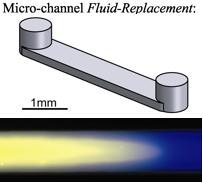
\includegraphics[height=1.5in]{Wells_and_Microchannels_2_Cropped.png}}&B)&\imagetop{\includegraphics[height=1.5in]{Zeta.pdf}}
\end{tabular}
\caption{\textbf{Fluid replacement in a microchannel}. A) Schematic of simple one-input-one-output microchannel and the characteristic parabolic shape of low Reynolds number fluid flow in microchannels. B) Washing constant, $\zeta$, plotted for various aspect ratios for microchannels with rectangular cross-section, $h/w$.}
\label{chap1:fig:washing}
\end{figure}

%%%%%%%%%%%%%%%%%%%%%%
%%%%%%%%%%%%%%%%%%%%%%
%%%%%        Evaporation       %%%%%%%
%%%%%%%%%%%%%%%%%%%%%%

\section{Evaporation: Theory and Implications}
\paragraph{Preface.}The information presented in this section is adapted or summarized from \cite{Berthier:2008jf,Berthier:2008tl}.\\
\\
\noindent Given the exposed fluid in passive-pumping-based devices, another question commonly fielded is, ``How do I keep evaporation from affecting my cells?'' Even in an incubator, a significant percentage of the microchannel volume can evaporate without additional measures. In previous work, we highlight that evaporation is surprisingly proportional to the radius of an exposed droplet instead of the surface area, as can be seen in Eq \ref{chap1:equ:evaporation} where $D$ is the diffusion coefficient of water vapor in air, $\Delta C_{sat}$ is the difference between the saturation concentration of water in air and the atmospheric concentration, and $R$ is the droplet radius.

\begin{equation}
E = \frac{2 \pi D}{\rho} \Delta C_{sat} R = \lambda R 
\label{chap1:equ:evaporation}
\end{equation}

In a passive-pumping-based channel, fluid typically flows from the smaller droplet to the larger droplet as seen in the top of Fig \ref{chap1:fig:evaporationSchematic}. However, as a evaporation begins to affect the volume of fluid in each drop, the surface tension attempts to keep the curvature at each port the same. This results in fluid flow back towards the input drop (Fig \ref{chap1:fig:evaporationSchematic}, bottom). This was first documented as a way to concentrate protein by Walker \etal\ and has since been used by Frisk \etal\ to increase the sensitivity of detection of botulinum neurotoxin \cite{Walker:2002oy,Frisk:2008pi}.

\begin{figure}[!ht]
\centering
\includegraphics[width=3.5in]{EvaporationSchematic.pdf}
\caption{\textbf{Evaporation-driven flow}. Schematic illustration of typical surface-tension driven flow using a pipette (top) and evaporation-driven flow (bottom).}
\label{chap1:fig:evaporationSchematic}
\end{figure}


From Eq \ref{chap1:equ:evaporation}, a dimensionless evaporation number, $Ev$, can be developed that represents the proportion of fluid that is lost over the time-course of an experiment for an array of droplets (see manuscripts for details) \cite{Berthier:2008jf,Berthier:2008tl}. Experiments validated this model which was then used to help characterize different ways to mitigate evaporation. As one might expect, in an array of droplets, the droplets at the perimeter incur the largest percent change in volume. Thus, for a given proportion of fluid lost from an array as predicted by the $Ev$ number, say 10\%, the majority of that 10\% is lost from the perimeter droplets. In this scenario, one can define a penetration depth of the evaporation effects. This penetration depth was numerically simulated and is shown in Fig \ref{chap1:fig:evaporation2} for different aspect ratio containers. From this information, it can be seen that the use of sacrificial fluid near the perimeter in low profile containers is an effective way to mitigate evaporation for passive-pumping-based devices. Further, the nesting of containers also adds another layer of protection against evaporation.

\begin{figure}[!ht]
\centering
\includegraphics[width=3.5in]{Evaporation_Exptl2.pdf}
\caption{\textbf{Evaporation from micro-device arrays}. Evaporation in containers of various aspect ratio used to house arrays of micro-devices with exposed fluid or droplets. For a given amount of fluid lost from the entire array (denoted by $Ev$), penetration depth is given for different \% losses. The penetration depth for 1\% of $Ev$ is roughly half the container radius for a container with an aspect ratio ($H/R$) of 0.1. Thus, all droplets outside a distance of $R/2$ are expected to see a loss of greater than 1\% of $Ev$.}
\label{chap1:fig:evaporation2}
\end{figure}

%%%%%%%%%%%%%%%%%%%%%%
%%%%%%%%%%%%%%%%%%%%%%
%%%%%        Reduced Volumes   %%%%%
%%%%%%%%%%%%%%%%%%%%%%

\section{Reduced Volumes: The Promise of Microfluidics}

\paragraph{Preface.}The information presented in this section is adapted or summarized from \cite{Warrick:2008rf}.\\
\\
\noindent One of the primary benefits of microfluidics is the reduced volumes needed to perform an assay, which can lead to reductions in assay footprints, cost, and the number of cells needed to perform an assay. This allows one to begin exploring larger parameter spaces with a given cell sample and is an important advantage in the areas of primary cell work and clinical diagnostics and will be important in addressing more complex biological hypotheses that require multi-parametric or combinatorial experimental designs. In this respect, Fig \ref{chap1:fig:scales} helps to put passive-pumping or tube-less microfluidics in perspective with other microfluidic approaches. Passive-pumping-based devices do not use the smallest volumes or have the highest potential for throughput but offer an important advantage similar to multi-well plates; they can be operated manually or integrated with existing pipette automation. This ability is very important for facilitating translation of new assays from the bench-top to the high-throughput screening facility. 

\begin{figure}[!ht]
\centering
\includegraphics[width=3.5in]{MicrofluidicsScales.pdf}
\caption{\textbf{Microfluidic platforms for screening}. Plot of approximate volumes-per-chamber across a range of spatial densities using different types of devices. The figure shows ranges of operation for traditional multi-well plates, tubeless microchannels, tubed/valved microchannels, and droplet-based devices (see Section X for descriptions and references). Tube-less microchannels can offer a reduction in volume-per-assay compared to multi-well formats of similar density but can still preserve the ability to individually address an assay compared to tubed/valved devices that use the same volume. Volume-per-assay increases for tubed/valved microchannels when implemented to individually address chambers due to increases in dead volumes, routing, tubing, or numbers of connected reservoirs, whereas multiplexing of fluid sources decreases the average volume-per-assay. Droplet-based fluidics typically deals with volumes below a few \textmu L and has the potential to manipulate picoliter volumes at high densities.}
\label{chap1:fig:scales}
\end{figure}

Besides increasing the number of experiments you can do with a given sample, the use of reduced volumes also affects the cellular microenvironment. As volumes reduce, the effective culture volume or ECV generally decreases (Fig \ref{chap1:fig:cellVolumeRatio}); that is to say, the volume of culture media per cell decreases. This decreased ECV gives the cell more control over its microenvironment. The cells can more quickly condition their microenvironment, resulting in more rapid accumulation and depletion of factors, nutrients, and waste. This effect has been used to increase the sensitivity of co-culture assays to uncover cell signaling effects that could not be seen before \invitro\ \cite{Domenech:2009jt}.

\begin{figure}[!ht]
\centering
\includegraphics[width=3.5in]{CellVolumeRatio.pdf}
\caption{\textbf{Effective culture volume (ECV) or volume-per-cell in 2-D and 3-D culture}. A) Schematic representation of cells uniformly seeded in 3-D culture and the associated ECV. $L$ is roughly the average spacing between cells. B) Example of different 2-D culture devices and their associate ECVs. The microchannel, tissue-culture flask, co-culture transwell, and 96-well plate in the photo are put in order of increasing ECV. If, in each case, the cells are plated at the same surface density upon the culture substrate (i.e., cells/mm ), then ECV is proportional to the fluid height over the cells.}
\label{chap1:fig:cellVolumeRatio}
\end{figure}

Lastly, by avoiding the use of tubes, passive-pumping-based microfluidics reduces `dead-volumes' and enables arrays of individually addressable devices. Individually addressable devices prevent any potential issues of `cross-talk' that can occur if the devices are connected in any way using tubing and valves. Another benefit is that interaction between devices is completely flexible and configurable via pipetting allowing fluid to be transferred at any time between any two channels.

%%%%%%%%%%%%%%%%%%%%%%
%%%%%%%%%%%%%%%%%%%%%%
%%%%%        Diffusion     %%%%%%%%%
%%%%%%%%%%%%%%%%%%%%%%
\section{Diffusion: Soluble Factor Signaling and Co-culture}

\paragraph{Preface.}This work was written in partnership with Erwin Berthier and represents a manuscript in preparation.\\
\\
\noindent Much in the same way that surface tension effects are more important on the micro-scale, so is diffusion. Across small distances diffusion can happen very quickly. In the case of synapses, factors diffuse to induce signaling in a matter of milliseconds. Given this difference, micro-scale technology has provided a variety of advanced techniques for tailoring the \emph{in vitro} microenvironment of cells to answer unique and specific questions that can be difficult or impossible to answer using macroscale analogs \cite{Chen:1998xq,Lucchetta:2005kn}. The area of segregated co-culture is particularly exciting given the increased sensitivity and flexibility of micro co-culture assays for examining soluble factor signaling between two or more cell types. Segregated co-culture in microdevices typically realize these improvements over standard macroscale technology (\emph{i.e.} transwells) through reduced signaling distances, the ability to precisely pattern cells, independent control of cell number \emph{v.s.} cell density, and increases in the number of cells per unit of culture volume \cite{Bhatia:1999ta,Domenech:2009jt,Folch:2000tb,Nelson:2002ev}. However, up to this point, more focus has been placed on providing unique capabilities instead of ways to objectively compare these new alternatives. Specifically, the literature is lacking a widely applicable tool for assessing the suitability of a particular device for a given co-culture scenario or for the reverse, providing insight into co-culture signaling dynamics based on culture results in a particular device design.

Analyses of soluble factor signaling in the literature are often aimed at very specific or detailed scenarios that are difficult to apply to other situations, even if closely related, while others can be too simplistic and cannot provide an adequate representation or are not tailored enough to the application of co-culture. The analysis provided here can be generalized to a wide range of relevant situations and considers the important but measurable characteristics of cellular sensitivity and soluble factor degradation. This method is a practical tool for both assessing the ability of co-culture device to support signaling between two cell populations as well as assessing the soluble factor production and sensitivity of cell types cultured using a particular device. In this way, the work presented here is significantly relevant and practical for both biologists and engineers and can also apply to other co-culture-like assays such as those for wound-healing or migration.

Fig \ref{chap1:fig:cocultureSchematic}A shows the major steps and processes involved in a paracrine interaction. Factors diffuse between cells through a gap ranging from nm's to mm's to initiate signaling. In the simplest case, a unique factor is produced\slash secreted\slash accumulated on one side and is received\slash sensed\slash taken up by the other (Fig \ref{chap1:fig:cocultureSchematic}A). 
\begin{figure}[!b]
\centering
\begin{tabular}{p{0.3cm}cp{0.3cm}c}
A)&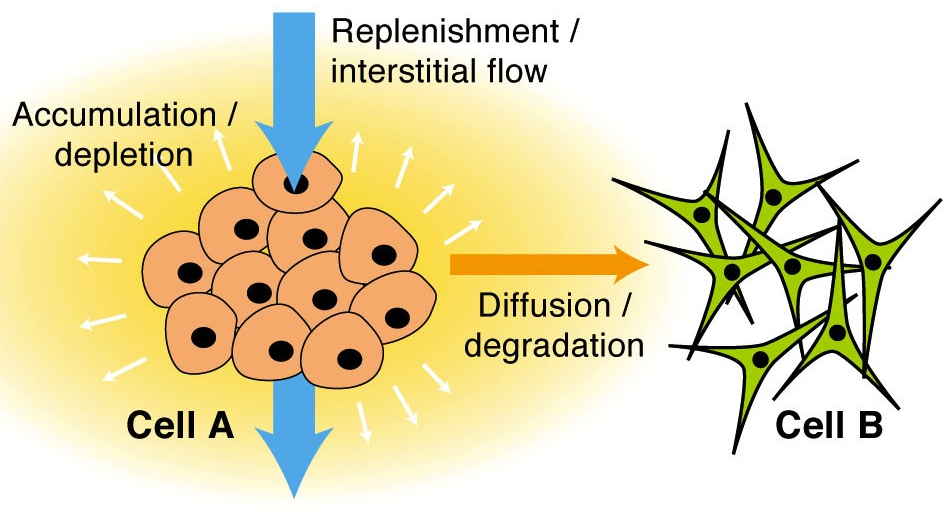
\includegraphics[width=2.5in]{DiffusionIntro_Cropped.jpg}&B)&\includegraphics[width=2.5in]{MathModel.pdf}
\end{tabular}
\caption{\textbf{Co-culture diffusion}. A. Schematic of the simplified coculture model used for analysis. The curvature in the concentration profile of the one dimensional model is evidence of degradation.}
\label{chap1:fig:cocultureSchematic}
\end{figure}
The processes of accumulation, transport, and depletion are dynamic, each with their own rate and associated timescale. There are also timescales and sensitivities associated with cell signaling and response. Design of co-culture assays must account for each of these timescales and sensitivities to enable robust observation of co-culture interactions between populations. Conversely, an understanding of these co-culture parameters can be used to give insight into the nature of an observed interaction in a particular device. Fig \ref{chap1:fig:cocultureSchematic}B is generalized schematic of how the soluble factor interactions of Fig \ref{chap1:fig:cocultureSchematic}A are modeled\slash studied \emph{in vitro} and forms the basis for a practical and widely applicable analysis of co-culture. Soluble factor \emph{transport} in the gap between the populations and the \emph{local culture environment} of the cells in each chamber will be modeled independently and linked in a discussion of timescales of co-culture signaling. A model of transport is developed first given the necessity of transport in paracrine interactions.

\subsection{Transport}
\subsubsection{Math Model}
\label{SubSubSection:MathModel}
The mathematical basis of the proposed transport model is described and used to compare the performance of multiple microscale co-culture devices. In the model shown in Fig \ref{chap1:fig:cocultureSchematic}B, there is a population of cells secreting a soluble factor that can be sensed by a population of receiving cells. In order to make the model both practical and applicable to a wide variety of situations, assumptions are made to simplify calculations and make it easier to estimate system parameters. First, it is assumed that the factor must reach a threshold concentration, $C_{thresh}$, in the receiving chamber in order for signaling to occur. Second, at steady-state, the secreting cells are able to maintain a local concentration of $C_{source}$. As the factors diffuse from one side to the other they also degrade (see curved lines in Fig \ref{chap1:fig:cocultureSchematic}B plot). We can model the process of diffusion and take into account degradation using Eq \ref{equ:diffusion} where $C$ is the concentration [mol/m$^{3}$], $k$ is the degradation constant [1/s], $D$ is the diffusion coefficient [m$^{2}$/s], and $x$ is the distance from the secreting cells [m]. We can use this model to evaluate device designs and determine for a particular factor whether signaling will be efficient or even possible. The 1-D model is most applicable for scenarios where the height and depth of the gap region is less than or equal to the height and depth of the culture chambers (Fig \ref{chap1:fig:cocultureSchematic}A).


%\begin{figure}[!t]
%\centering
%\includegraphics[width=3.2in]{cocultureAnalysis.jpg}
%\caption{Analytical results using a simplified model of segregated coculture. A. The ratio of the actual exchange rate of soluble factors to the maximum possible exchange rate for various geometries and diffusion coefficients is plotted. The ratio is calculated for a ratio of $C_{thresh}/C_{source}=0.1$. B. Plot of $L_/L_{\tau}$ when $\dot{N}_{L}/\dot{N}_{max} = 0$ (\emph{i.e.}, when soluble factor exchange is 0 but the concentration over the sensing cells is able to reach $C_{thresh}$. Thus, this represents the maximum possible distance over which signaling can occur for a particular coculture scenario, $L_{max}/L_{\tau}$. The dotted line represents $L_{max}/L_{\tau}$ when $C_{thresh}/C_{source}=0.1$ -- the same scenario as plotted in part A.}
%\label{chap1:fig:coculture}
%\end{figure}

\begin{equation}
\frac{\partial C}{\partial t} = D\,\frac{\partial^{2} C}{\partial x^{2}} - k C
\label{equ:diffusion}
\end{equation}

We are interested finding $\dot{N}_{L}$, the flux of molecules into the receiving culture chamber (i.e. the number of moles being delivered per unit time at $x=L$, where $L$ is the distance between the two cultures). $\dot{N}_{L}$ is given by Eq \ref{equ:ficks} in terms of the characteristic parameters of the co-culture system. The dimensionless coefficient $\alpha$ varies between 0 and 1 and represents how much degradation of the diffusing molecules attenuates flux. $D$ describes the influence of the medium through which a particular molecule diffuses (e.g. a molecule diffuses more quickly through typical cell culture media than a collagen matrix). The quantity $A/L$ represents the influence of geometry (i.e. more flux occurs through a short channel with a large cross-section versus a long and narrow channel) whereas $\Delta C$ encompasses the influence of the cells on the system.

\begin{equation}
\dot{N}_{L} = \alpha \, D \left(\frac{A}{L} \right) \Delta C
\label{equ:ficks}
\end{equation}

\begin{equation}
\Delta C = C_{source}-C_{thresh}
\label{equ:deltaC}
\end{equation}

\begin{equation}
\alpha=\frac{\mathcal{L}}{1-\mathcal{C}}\left(\frac{1-\mathcal{C}\cosh(\mathcal{L})}{\sinh(\mathcal{L})}\right)
\label{equ:alpha}
\end{equation}

\begin{equation}
\mathcal{C} = \frac{C_{thresh}}{C_{source}}
\label{equ:C}
\end{equation}

\begin{equation}
\mathcal{L} = \frac{\sqrt{k}L}{\sqrt{D}} = 1.18\frac{L}{L_{\tau}} = \frac{\sqrt{ln(2)}}{\sqrt{\tau}}\frac{\,L}{\sqrt{D}}\frac{\sqrt{2}}{\sqrt{2}} = 1.18\frac{L}{\sqrt{2 D \tau}} = 1.18\frac{L}{L_{\tau}}
\label{equ:L}
\end{equation}

\begin{equation}
L_{\tau}= \sqrt{2 D \tau}
\label{equ:lTau}
\end{equation}

When the solution to $\dot{N}_{L}$ is put into this form, it can be seen that the influence of degradation on co-culture signaling (i.e. the value of $\alpha$) depends upon two important dimensionless parameters, $L/L_{\tau}$ and $C_{thresh}/C_{source}$ (Eq \ref{equ:alpha}-\ref{equ:lTau}). The distance $L_{\tau}$ represents the average distance a molecule will diffuse in one half-life (Eq \ref{equ:lTau}). The half-life of the molecule, $\tau$, is given by ln(2)/$k$ where $k$ is the degradation rate in Eq \ref{equ:diffusion}. When $L/L_{\tau} \approx 0$, degradation is negligible, and when $L/L_{\tau} > 1$, degradation of the soluble factor significantly diminishes the rate of delivery to the receiving cells. The ratio of $C_{thresh}/C_{source}$ for a given $L_{\tau}$ determines the maximum possible distance at which signaling can be maintained, $L_{max}$ (Eq \ref{equ:lMax}). Beyond a distance of $L_{max}$, concentration of the factor falls below $C_{thresh}$ due to degradation, cutting off signaling. Lastly, the time it takes for a signal to travel a distance $L$ is approximately $L^{2}/(10\,$D) while the time it takes to reach equilibrium over that distance is roughly $L^{2}/(2\,$D).

\begin{equation}
L_{max} = 0.85 \, L_{\tau} \, \textrm{arccosh}\left(\frac{1}{\mathcal{C}}\right)
\label{equ:lMax}
\end{equation}

The only non-linear term in the calculation of $\dot{N}_{L}$ is $\alpha$, which is plotted in Fig \ref{chap1:fig:alpha} for a range of $L/L_{\tau}$ and $C_{thresh}/C_{source}$. This information is will be used to compare different co-culture device designs.

\begin{figure}[!t]
\centering
\includegraphics[width=3.2in]{Alpha.pdf}
\caption{\textbf{Degradation coefficient, $\alpha$}. Plot of $\alpha$, for different values of $L/L_{\tau}$ and $C_{thresh}/C_{source}$. Black triangles indicate the maximum signaling distance that can be maintained for each value of $C_{thresh}/C_{source}$ (i.e. $L_{max} = 2.5 L_{\tau}$ for $C_{thresh}/C_{source}$ = 0.1).}
\label{chap1:fig:alpha}
\end{figure}

\subsubsection{Comparison of Device Designs}

\def\imagetop#1{\raisebox{1em}{\vtop{\null\hbox{#1}}}}
\begin{table*}[!t]
\caption{\textbf{Comparison of soluble factor delivery in various microscale co-culture designs}. Comparisons are made for a generic short half-life soluble factor ($\tau=30$ [min], D = 100 [$\mu$m$^{2}$/s] in media). The last column, $\dot{N}_{L}/d$, is the rate of molecular transport into the receiving culture chamber \emph{per unit length} $d$. The length $d$ is measured along the length of the interface between the two cultures. The delivery rates can be used to estimate the efficacy of each design relative to one another. Calculations assume $C_{thresh}/C_{source}=0.1$.}%$L_{max}$ for this scenario is 880 $\mu$m.
\centering
\begin{tabular}{p{2cm}@{\,}p{2.7cm}@{\,}p{3.2cm}@{\,}>{\centering}p{1.2cm}@{\,}>{\centering}p{1.2cm}@{\,}>{\centering}p{1.5cm}@{\,}>{\centering}p{1cm}@{\,}>{\centering}p{2cm}}\toprule Method & Embodiment & Schematic & Height\newline$h$\newline[$\mu$m] &  Length\newline$\;\;L$\newline[$\mu$m] & Diff. Coeff.\newline D\newline[$\mu$m$^{2}$/s] & Deg. Coeff.\newline$\alpha$ & Delivery Rate\newline$\;\;\dot{N}_{L}/d$\newline[pmol/(m\,s)] \cr \midrule
Laminar flow patterning & \imagetop{\includegraphics[height= 1.4cm]{LaminarMethod.pdf}} &\imagetop{\includegraphics[height=1.4cm]{LaminarSchematic.pdf}} & 250 & 250 & 100 & 0.95 & 95$\,\Delta C$ \cr 
Segregated co-culture & \imagetop{\includegraphics[height= 1.4cm]{SegregatedMethod.pdf}} &\imagetop{\includegraphics[height= 1.4cm]{SegregatedSchematic.pdf}} & 12.5 & 500 & 100 & 0.81 & 2.0$\,\Delta C$ \cr 
Gel-separated co-culture & \imagetop{\includegraphics[height= 1.4cm]{GelMethod.pdf}} &\imagetop{\includegraphics[height= 1.4cm]{GelSchematic}} & 250 & 750 & 20 & 0 & 0$\,\Delta C$ \cr 
\bottomrule
\end{tabular}
\label{tab:examples}
\end{table*}

Using this model, we can practically and objectively compare different device designs for a particular co-culture scenario (Tab \ref{tab:examples}). In order to compare the transport of soluble factor in each device, a value is calculated for $\dot{N}_{L}$. However, the length of the interface between the cell populations ($d$) is different for each device. For this reason, we present the rate of transport per unit length of the device (i.e. $\dot{N}_{L}/d$). The devices are compared assuming the factor of interest is a relatively short-lived protein with a diffusivity typical of many growth factors ($\tau$ = 30 [min], D = 100 [$\mu$m$^{2}$/s]). It is also assumed that the secreting cells produce a relative abundance of the factor compared to the sensitivity of the receiving cells (i.e. $C_{thresh}/C_{source}$ = 0.1).

% Table Calcs for alpha
%(sqrt(2*100e-12*30*60))
%    r151 = 0.0006
%1.18/r151
%    r152 = 1966.66666667
%((250e-6*r152)/(1-0.1))*((1-0.1*cosh((250e-6*r152)))/(sinh((250e-6*r152))))
%    r154 = 0.947653018885
%((500e-6*r152)/(1-0.1))*((1-0.1*cosh((500e-6*r152)))/(sinh((500e-6*r152))))
%    r153 = 0.805564568799
%(sqrt(2*20e-12*30*60))
%    r148 = 0.0002683281573
%1.18/r148
%    r149 = 4397.60035575
%((750e-6*r149)/(1-0.1))*((1-0.1*cosh((750e-6*r149)))/(sinh((750e-6*r149))))
%    r150 = -0.0962824670932

%Table Calcs for Ndot/d = alpha D h / L
% 0.947653018885*100*250/250
% 0.805564568799*100*12.5/500
% 0*20*250/750

The highest transport per unit length (95$\Delta C$) was calculated for the case of laminar flow patterning where the cell populations were in close proximity and with little or no constriction or barrier to diffusion between them. Degradation of the short half-life molecule was negligible ($\alpha \approx 1$). By constricting the region between cells and doubling the distance between the cells, transport was cut by factor of 1/50 (see segregated co-culture). Degradation was not the major factor in the segregated case; instead, the constriction used to separate the populations severely limited transport. In the case of the gel-separated co-culture, $\alpha$ was $\le 0$, suggesting that signaling is impossible in this scenario. Diffusion of the factor in gel is significantly slower than in media such that, over a distance of 750 $\mu$m, the secreting cells could not produce a concentration $\ge C_{thresh}$ in the receiving cell culture chamber due to degradation.

Although some devices prove more effective than others in this example, other situations might prove the designs to be relatively interchangeable, such as with small, long lived molecules like hormones. There is also the question of timing. Can the molecule accumulate to appropriate concentrations and diffuse to the receiving population in a short enough time to observe cell response upon acquiring a specific readout? Will uptake or media replenishment significantly attenuate signaling? To begin answering these questions, the local environment of each cell population is examined.

%$\dot{N}_{L}$ depends on the cross sectional area of the gap region, $A$; diffusion coefficient, D; characteristic length ratio, $L/L_{\tau}$; and ratio of the receiving chamber concentration to the source chamber concentration, $C_{thresh}/C_{source}$. $C_{thresh}$ is used for the concentration in the receiving culture chamber because the goal of the co-culture device is to adequately supply the receiving cells with enough factor to illicit a response and very often a threshold concentration can be associated with this response. When $\alpha$ approaches 1, degradation is insignificant and exchange is maximal. When the value approaches 0, either the constriction\slash barrier between the culture chambers or degradation of soluble factors over the distance $L$ is preventing significant transport. When the value actually reaches 0, a value of $C_{thresh}$ can no longer be sustained in the receiving culture chamber, making signaling impossible. 

%$\dot{N}_{L}/\dot{N}_{max}$ can be used to compare devices in two ways. The first way compares performance relative to a common $\dot{N}_{max}$ (the higher of the two $\dot{N}_{max}$'s calculated for each device) and the other uses values of $\dot{N}_{max}$ that are specific to each device. The first method is a direct comparison of specific geometries while the second allows one to compare devices if they were to be scaled such that the culture chamber heights were the same. In this way, the second is more appropriate for comparing methods rather than specific device designs, such as the use of constrictions \emph{vs} gel barriers to segregate populations. In order to compare two devices with different geometries, one can calculate $\dot{N}_{L}/\dot{N}_{max}$ If two different devices have the same value of $\dot{N}_{L}/\dot{N}_{max}$, then they can equally support soluble factor signaling for a given co-culture scenario if the culture chamber heights were made to be similar.

%A simple graphical method is provided to perform these comparisons using only the heights of the culture chamber and gap region as well as the diffusion coefficient and half-life of the molecule of interest.

%Within the plot of $\dot{N}_{L}/\dot{N}_{max}$ in Fig \ref{chap1:fig:cocultureSchematic}A, colored and numbered dots are plotted that represent the efficiency of soluble factor exchange for each device shown in Fig \ref{chap1:fig:cocultureSchematic}B for two different factors -- one with a short half-life and one with a long half-life. Given the disparity of the points, one can begin to seen that soluble factor exchange can be dramatically different depending on the molecule and coculture geometry. The plot shows that the LFP device presented here (device 1) produces nearly maximal exchange of factors and avoids issues of factor degradation. On the contrary, \mbox{IL-2} signaling is impossible in device 3 as $L/L_{\tau}$ is greater than $L_{max}/L_{\tau}$. 

\subsection{Local Culture Environment}

Although transport between the cell populations is critical for observing soluble factor interactions, it is also important to understand the dynamics of the local environments of each population in culture as they determine the boundary conditions of the transport model from the previous section (i.e. $C_{thresh}$ and $C_{source}$). We can use well-studied models of soluble factor secretion and uptake to give a sense of these dynamics for designing co-culture assays. Models of platelet-derived growth factor (PDGF) accumulation and epidermal growth factor (EGF) depletion will be used for this purpose and are discussed along with the influence of cell density. The models approximate the local environment of a cell in 2-D culture (i.e. culture on a flat substrate instead of in a 3-D matrix) as being a cylinder where the radius of the cylinder depends upon the cell density and the height of the culture chamber (Fig \ref{chap1:fig:diffusionGeom}, see Appendix \ref{App:Diffusion} for description of simulation methods).

The PDGF and EGF models in this section require 3-D diffusion modeling (COMSOL modeling sofware, Burlington, MA) and the knowledge of factor production/uptake rates, which can be difficult to measure. Therefore, the intent is not to describe to the reader how to do this type of modeling; instead, the examples will be used to discuss the timescales of accumulation and depletion and how different parameters affect those processes. In this way, some practical guidelines can be suggested from specific examples. Also, these models examine the dynamics of a single culture chamber and do not account for transport between two culture chambers. The interaction between culture chambers depends on the conditions in each chamber as $C_{source}$ and $C_{thresh}$ determine the boundary conditions of the co-culture signaling model. Further, the time-scale of accumulation and depletion within each chamber determine when co-culture signaling is likely to occur.

\begin{figure}[!t]
\centering
\includegraphics[width=3.5in]{CylindricalChannel.pdf}
\caption{\textbf{Cylindrical diffusion model geometry}. The cylindrical geometry in the schematic used to estimate the case of a single cell in culture with neighbors on a 2-D substrate. The geometry is modeled in COMSOL using a 2-D axis symmetrical model with a flux boundary condition at the cell surface defined as $q$. The area of the base of the unit-cylinder is equal to the area-per-cell on the substrate of the channel. Parameters of the model were determined from the literature and noted in figure captions.}
\label{chap1:fig:diffusionGeom}
\end{figure} 

\subsubsection{PDGF Accumulation}

Fig \ref{chap1:fig:PDGF} shows modeling results for fibroblastic cells (10$\mu$m in diameter) producing platelet-derived growth factor (PDGF) at a rate, $q$, reported in simulations and experimental work from the literature (cite Lauffenburger - cell density and Leof). Concentration is plotted with time for the cell boundary, $C_{cb}$; the ceiling of the channel (i.e. approximately the point of lowest concentration); and the average concentration over the entire channel. The simulation assumes that cells are seeded at 300 cells/mm$^{2}$ ($\sim 30\%$ confluency or $\sim 65$ $\mu$m spacing). The channel height, $H$, is chosen to be 250 $\mu$m ($\gg$ the $5\mu$m cell radius). Although the dissociation constant of PDGF to its receptor does not always predict the concentrations necessary for cellular response, it is used here to estimate a cellular threshold concentration, $C_{th}$. Initially, the concentration near the cell builds quickly showing local accumulation of the factor. However, soon the difference between the average channel concentration and the cell boundary concentration stabilizes at $t_{d}=H^{2}/(2\,D)$. Each measure of concentration then rises at a rate of $q/V$ where $V$ is the volume of the modeled cylinder. 


\begin{figure}[!b]
\centering
\includegraphics[width=3.5in]{PDGF.pdf}
\caption{\textbf{Production of PDGF by fibroblasts.} Plot of concentration with time for the parameters listed in the plot. Parameters are taken from \cite{Lauffenburger:1989fy,LEOF:1986uq} (see Appendix \ref{App:Diffusion} for more details).}
\label{chap1:fig:PDGF}
\end{figure}

The average concentration in the channel reaches $C_{thresh}$ in $\le 30$ min, at which point the concentration at the cell boundary is $\sim 35\%$ higher. However, this percent difference quickly becomes negligible as PDGF continues to rapidly accumulate. The calculations here assume there is no depletion due to adsorption, absorption, uptake, degradation, or cellular feedback mechanisms that might reduce production. Despite these assumptions, it becomes apparent that the cells in this microscale culture model can quickly affect their local environment due to a high cell to culture-volume ratio (i.e. the culture chamber height is small). If the height of the fluid over the cells were to be like that in a typical culture flask (2 mm), accumulation would occur 8 times slower (2 mm / 0.25 mm = 8). Thus, instead of reaching $C_{thresh}$ in just 30 min, it would take approximately 4 hours in a culture flask.

\subsubsection{EGF Depletion}

\begin{figure}[!b]
\centering
\includegraphics[width=3.5in]{EGF.pdf}
\caption{\textbf{Uptake of EGF by fibroblasts.} Plot of concentration with time for the parameters listed in the plot. The geometry of the simulation is shown in Fig \ref{chap1:fig:diffusionGeom}. Parameters are taken from \cite{KNAUER:1984fj,STARBUCK:1992kl} (see Appendix \ref{App:Diffusion} for more details).}
\label{chap1:fig:EGF}
\end{figure}

Fig \ref{chap1:fig:EGF} shows the reverse case of EGF uptake of by human fibroblasts (HFs). The same parameters exist for the EGF example as for the PDGF example, but with different values. The production rate is negative here to signify uptake rather than release. Also, although the dissociation constant of EGF to its receptor is often quoted as $10^{-10}$ to $10^{-9}$, it has been observed that the apparent cellular affinity for EGF is $\sim 4.69 \times 10^{-11}$, possibly due to cellular regulation of surface receptors (cite Lauffenburger). The initial concentration of EGF in the culture medium is chosen to be $4 \times C_{th}$ for illustrative purposes. The plot shows that cells uptake the EGF linearly until concentrations approach $C_{th}$ whereupon the sigmoidal response of the cell is observed to reduce uptake due to depletion of the medium. Thus, it can be seen that cellular uptake rates for small values of $V$ can cause rapid depletion of threshold levels of factor. The medium becomes significantly depleted $< 1$ [hr] after reaching $C_{th}$. This time is relatively short compared to the 6-8hrs of exposure often required to illicit a growth response. Therefore, when $V$ is too small, depletion can make it impossible to examine dose response to steady concentrations of soluble factors. However, if the initial concentration, $C_{0}$, is high enough initially, saturating exposure can be achieved for significant periods of time until the threshold concentration is reached whereupon depletion quickly occurs.

\subsubsection{Single Chamber Accumulation/Depletion and Local Cell Density}
\label{SubSubSection:LocalGradients}

As mentioned in the previous examples, local concentration is significantly affected by seeding density or cell spacing. Since the total volume of the channel is constant, the rate of accumulation increase linearly with the number of cells seeded into a chamber. This also means that normal random dispersion on the culture substrate can significantly affect local accumulation and depletion. Locally (i.e. within the neighborhood of a group of cells), accumulation\slash depletion rates can vary by many multiples due to cell slumping that arises from the stochastic nature of cell suspensions and seeding or by the natural growth and reorganization of cells during culture. However, the influence of these local variations is quickly diminished given that the average concentration in the channel can quickly surpass threshold concentrations or can be quickly depleted, thereby homogenizing cell-response throughout the chamber.

\subsection{Co-culture Timescales}

Four important timescales to consider for the study of co-culture interactions are the time for accumulation in the secreting chamber, the time for diffusion across the gap, the half-life of the molecule, and the timescale of the phenotypic change to be measured in the receiving chamber. The times are listed in this order as they mirror the typical sequence of events from secretion, to transport and degradation, to uptake and response. If any of these timescales does not agree with the readout or limits the process of soluble factor signaling, it is possible that the device geometry might be changed to minimize this constraint and enable more robust signaling. Further, geometric changes might be used to modulate a signaling event to gain additional insight.

Methods are available to estimate these times, especially when testing the effects of a specific factor. Accumulation times per volume of fluid can typically be estimated using an ELISA or other similar readout. A diffusion coefficient is necessary and can typically be estimated using the molecular weight of the molecule if no information is available in the literature (see Einstein–Stokes equation). However, a typical 20kD protein is usually in the range of 100 \textmu m$^{2}$/s in fluid similar to media or water. A time for diffusion can then be estimated as $t_{d} = L^{2}/(2D)$ where $L$ is the distance of interest such as the gap width. Half-life information can often be found in the literature as well but can also be measured for secreted factors using an ELISA. If diffusion times across the gap are on the order of degradation times, it is worth performing the analysis outlined and described in Section \ref{SubSubSection:MathModel}. The $C_{source}$ needed for the analysis in that section can come from the ELISA accumulation data whereas the $C_{thresh}$ is more easily determined from dose-response curves obtained in mono-culture using an exogenous source of the protein. The dose-response data also will likely provide the time-scale of the phenotypic response being measured. The co-culture assay should be performed over a long enough time to allow accumulation, transport, and response.

If the factor is unknown, different designs can be used to alter these timescales and gain in general information about the unknown factor. For example, if signaling is achieved, one can assume that the degradation coefficient, $\alpha$, of Section \ref{SubSubSection:MathModel} is $>$ 0. The value of $\alpha$ can then be estimated for potential candidate molecules to narrow the scope of further inhibition studies to identify the factor. If one can observe a difference in response using narrow and wide gaps, one can support hypotheses of the size or degradation rate of the putative factor. By using different culture chamber sizes to vary the ratio of secreting and receiving cells, insight into secretion rates and sensitivity of the receiving cells can be gained. However, basic considerations of waste production and nutrient depletion can also change when exploring these various permutations. Also, in contrast to the discussion in Section \ref{SubSubSection:LocalGradients}, factor concentrations and response within the receiving chamber can be inhomogeneous and lead to further insight, as explained below.

The results shown in Tab \ref{tab:examples} illustrate that delivery of a co-culture factor to the receiving cell chamber can sometimes be quite limited. In the receiving chamber, the gap acts like a localized source of factor where the factor must diffuse throughout the receiving chamber to influence the population. Depending on the distance of a cell from the gap, the cell could experience a concentration of factor significantly different than its neighbors closer or farther from the gap. This local gradient is different than the local gradient of the previous subsection on accumulation and depletion. In this case, the limited flux through the gap can result in a gradient of factor within the dose-response range of the receiving cells that can last for significant periods of time or potentially reach a quasi-steady-state. For this reason, a dose response may be observed within the receiving chamber. If cells are in close proximity to the gap, diffusion times will be reduced, limiting the potential for these gradients. If the flux through the gap is relatively large, accumulation in the receiving chamber will occur more quickly and help to homogenize response as well.

\subsection{Other Microenvironmental Considerations}
Microscale devices are often made of materials that are different from macroscale tools. Different materials and the reduced scale of the culture devices can lead to changes in the microenvironment that are important to be aware of. A common material for micro-devices is polydimethylsiloxane, which has been shown to have a high capacity for absorbing small lipophilic molecules such as estrogen, an important soluble factor in many disease models \cite{Regehr:2009fk}. Also, the surface to volume ratio of micro-devices is significantly increased. Thus, adsorption alone can significantly deplete low concentrations of soluble factors \cite{Lionello:2005zh}.

\subsection{Conclusions}
Microscale techniques offer new ways to probe soluble factor signaling interactions and dynamics with increased sensitivity yet we lack accessible, informative, and widely applicable methods to assess these interactions. These types of analysis methods are needed to aid design and interpretation of co-culture devices and assays to further leverage the potential advantages of microscale co-culture. A model and discussion of co-culture transport was provided here to address this need. The model includes source and threshold concentrations of factor as well as degradation, an often overlooked but important part of soluble factor signaling regulation. By including these components into the model, the analysis gains accuracy and flexibility while avoiding the complexity of more involved methods of analysis. The influence of degradation is summarized in a single dimensionless value that can be estimated from the equations and plot provided. Each parameter of the system can be estimated from the literature or via standard ELISA experiments. Devices were compared using the model and illustrate the importance of micro-device geometry in promoting robust co-culture signaling. The importance of four different timescales (accumulation\slash depletion, transport, degradation, and cell response) were discussed, highlighting how each can be used in aiding design of co-culture devices as well as how they can be used to interpret co-culture results and observations.  

%\section{Extras}
%\clearpage
%
%%%%%%%%%%%%%%%%%%%%%%%%
%
%\paragraph*{Cell:Volume Ratio and Diffusion Distances.}Cell:volume ratio refers to the number of cells being cultured to the volume of media in which they are being cultured. The cell:volume ratio in microscale devices is typically 4 - 10 times higher in microscale culture devices than more standard devices such as culture flasks or micro-well plates. Increased cell:volume ratios allow soluble factors to build up more rapidly. This means that dilution of signaling molecules is prevented and biologically relevant concentrations of these factors are reached more quickly.
%
%The diffusion distance between two cell populations in co-culture is an important consideration given the short half-lives of many siganling molecules (\emph{e.g.}, IL-2, 7 min; slkdfjlskdf). Given the half life of a particular molecule ($\tau$), the distance the molecule can diffuse during a single half life ($L_{\tau}$) can be estimated using $L_{tau} = \sqrt{2 D \tau}$, where $D$ is the diffusion coefficient. Given that typical diffusion coefficients for soluble factors are on the order of 100 \textmu m$^{2}$/s and half lives range from 0.1-2 hours, typical values for $L_{\tau}$ are $\sim$250 - 1200 \textmu m. 
%
%\paragraph*{Maximizing Exchange of Soluble Factors.}The extent of soluble factor exchange between the patterned cell populations can be modulated by adjusting the distance between them or by changing the height of the region in the space between populations. These parameters are illustrated in a cross-section view of a basic microchannel co-culture device (Fig \ref{chap1:fig:coculture}). The co-culture system can be roughly approximated as having one concentration in the region near the producing cells and a second concentration near the receiving cells with a difference of $\Delta C$. Employing Fick's Law of diffusion, Eq \ref{equ:ficks} can be used to relate the molecular transport rate ($\dot{N}$, [mol/s]) between the populations to the concentration gradient ($\partial C/\partial x$) and the cross-sectional area (A) through which the molecules must diffuse to reach the other side. 
%
%\begin{equation}
%\frac{\partial C}{\partial t} = D\,\frac{\partial^{2} C}{\partial x^{2}} - k C
%\end{equation}
%
%\begin{equation}
%\dot{N} = D\,\frac{\partial C}{\partial x} A
%\end{equation}
%
%\begin{equation}
%\dot{N}_{max} = D\,\frac{\Delta C}{L} A
%\end{equation}
%
%\begin{equation}
%\textrm{half-life} = \tau = \frac{\ln(2)}{k}
%\end{equation}
%
%\begin{equation}
%\mathcal{L} = \frac{\sqrt{k}L}{\sqrt{D}} = \frac{\sqrt{ln(2)}}{\sqrt{\tau}}\frac{\,L}{\sqrt{D}}\frac{\sqrt{2}}{\sqrt{2}} = 1.18\frac{L}{\sqrt{2 D \tau}} = 1.18\frac{L}{L_{\tau}}
%\end{equation}
%
%\begin{equation}
%\mathcal{L}_{max} = \textrm{arccosh}\left(\frac{1}{\mathcal{C}}\right) %= -\ln\left({\frac{C_{1}}{C_{2}}-\sqrt{\left(\frac{C_{1}}{C_{2}}\right)^{2}-1}}\right) = \textrm{arccosh}\left(\frac{C_{1}}{C_{2}}\right) 
%\end{equation}
%
%\begin{equation}
%L_{\tau}= \sqrt{2 D \tau}
%\end{equation}
%
%\begin{equation}
%\mathcal{\dot{N}_{\mathrm{L}}}=\frac{\dot{N}_{L}}{\dot{N}_{max}}= \frac   {\left(D \frac{\partial C}{\partial x}A\right)\big|_{x=L}}   {\left(D \frac{\Delta C}{L} A\right)}
%\end{equation}
%
%\begin{equation}
%\mathcal{A}=\frac{A}{A_{max}}
%\end{equation}
%
%\begin{equation}
%\mathcal{C}=\frac{C_{2}}{C_{1}}
%\end{equation}
%
%\begin{equation}
%\mathcal{\dot{N}_{\mathrm{L}}}=\frac{\mathcal{A}\mathcal{L}}{1-\mathcal{C}}\left(\frac{1-\mathcal{C}\cosh(\mathcal{L})}{\sinh(\mathcal{L})}\right) = \mathcal{A}\alpha
%\end{equation}
%
%%\begin{equation}
%%\frac{\dot{N_{2}}}{\dot{N_{2,max}}}=\frac{h}{h_{max}}\frac{\frac{L}{L_{\tau}}}{1-\frac{C_{1}}{C_{2}}}\left(\frac{1-\frac{C_{1}}{C_{2}}\cosh(\frac{L}{L_{\tau}})}{\sinh(\frac{L}{L_{\tau}})}\right)
%%\end{equation}
%%\begin{equation}
%%\frac{\dot{N_{2}}}{d}=D\frac{\alpha h}{L}\left(\frac{C_{1}-C_{2}\cosh(\alpha)}{\sinh(\alpha)}\right)
%%\end{equation}
%%\begin{equation}
%%C_{a}+C_{b} = C_{1}
%%\end{equation}
%%\begin{equation}
%%C_{b} = \frac{C_{1}e^{\frac{L} {\sqrt{\tau D}}}-C2}   {e^{\frac{L} {\sqrt{\tau D}}}-e^{\frac{-L} {\sqrt{\tau D}}}}
%%\end{equation}
%%\begin{equation}
%%C_{a} = C_{1} - \frac{C_{1}e^{\frac{L} {\sqrt{\tau D}}}-C2}   {e^{\frac{L} {\sqrt{\tau D}}}-e^{\frac{-L} {\sqrt{\tau D}}}}
%%\end{equation}
%
%%h = 1;
%%C = 0.01;
%%L = linspace(0,5,50);
%%Ratio = (h).*(L).*(1/(1-C)).*((1-(C).*cosh(L))./(sinh(L)));
%%plot(L,Ratio);
%%drawnow;
%
%
%k is the degradation rate (i.e. 0.1 of C is degraded per unit time)
%
%
%For a given $\Delta C$, as the distance between the cells decreases (\emph{i.e}, $\Delta x \downarrow$) the amount of soluble factor that gets delivered per unit time to the other side increases. By keeping the height of the microchannel between the groups of cells equal with the height of the culture regions, transport of signaling factors between the populations is maximized. Similarly, the use of gel barriers or filters increase the resistance to transport by either changing the effective value of $D$ or $A$. Using the patterning method of Fig \ref{chap1:fig:experimental2}, the space between the cells and resistance to diffusive transport are much reduced compared to transwell assays and help to establish effective soluble factor communication in co-cultures.
%
%\subsection*{Important Identities}
%
%\begin{equation}
%2\cosh (\beta) = e^{\beta}+e^{-\beta}
%\end{equation}
%
%\begin{equation}
%2\sinh (\beta) = e^{\beta}-e^{-\beta}
%\end{equation}
%
%\begin{equation}
%\mathrm{arccosh} (\beta) = \ln\left(\beta + \sqrt{\beta^{2} - 1}\right)
%\end{equation}
%
%%can also be adjusted to modulate the amount of soluble factor exchange as well as . This can be seen using Fick's Law of diffusion which can be used to calculate the moles of soluble factor delivered per unit time ($\dot{N}$) at steady-state from one group of cells to another .

\chapter{Components: `The Flux Capacitor' for Pipete-Based Laminar Flow Patterning}

\section{Preface}
Contents of this chapter are taken from \cite{Berthier:2011fk} which was written in equal part with Erwin Berthier.

\section{Introduction}
Laminar flow patterning (LFP) is a prominent and established method used in microfluidics to pattern cells, particles, and treatments within a single channel \cite{Takayama:1999qf}. The method can be used to precisely control the nature and location of an interface between two miscible or non-miscible fluids, without requiring a physical divider \cite{Lucchetta:2005kn}. In addition, the laminar behavior of fluids at the microscale allows diffusion to be leveraged as a highly controllable mixing force enabling the creation of precise gradients within a microchannel \cite{Sia:2003bh}. The method has also been leveraged in areas such as the dynamics of chemical and enzymatic reactions \cite{Regenberg:2004ly} and the response of cell cultures to patterned treatments \cite{Tourovskaia2005Differentiation}. LFP has proven to be an enabling method for microfluidic cell-based assays where it is predominantly used for generating gradients of soluble factors in chemotaxis assays \cite{Li-Jeon:2002uz}, but is also used in the study of soluble factor signaling between different cell compartments \cite{Torisawa:2009bh,Sung:2010fk}, and for patterning a gap between two cell culture populations in wound-healing/invasion assays \cite{Wong:2008lq}.

\begin{figure}[!b]
\centering
  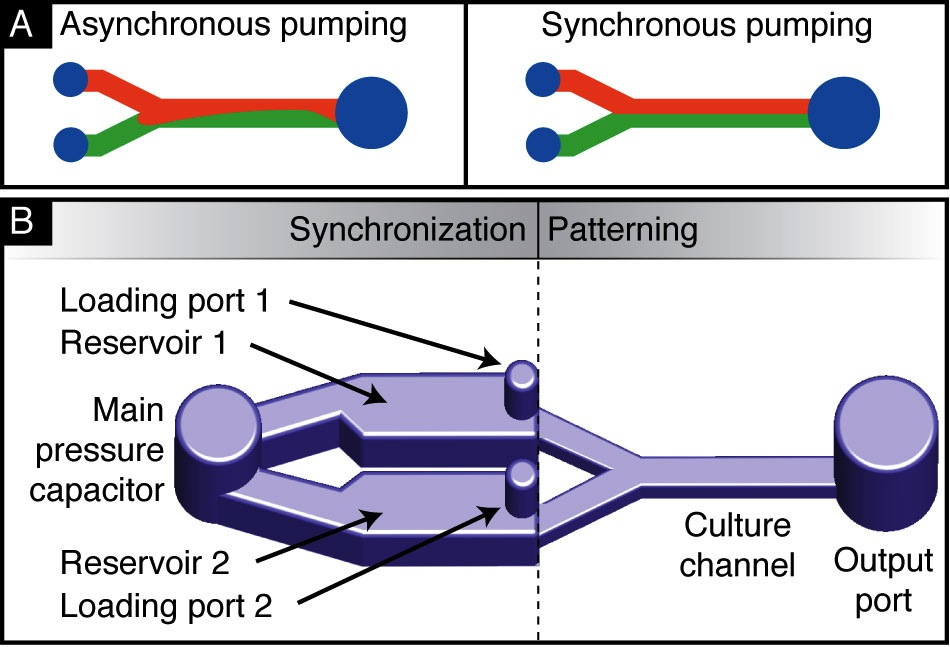
\includegraphics[width=8cm]{figure1.jpg}
  \caption{\textbf{The flux capacitor}. A. Flow pattern in a laminar flow patterning channel with unsynchronized pressures (left) and synchronized pressures (right). B. Schematic of the proposed synchronization method. A fluidic capacitor links the two sample loading ports of the Y-channel. The capacitor acts as a temporary destination for loaded fluid and balances the pressure applied to each branch for laminar flow patterning.}
  \label{fig:scematic}
\end{figure}

Despite the multitude of applications demonstrated using LFP, use of the method has not spread further than a restricted number of microfluidic labs, especially for applications where only a brief period of laminar flow is needed (\emph{i.e.}, in short-term LFP applications such as transient gradients or cell patterning). In short-term LFP applications, the complexity and expertise required to connect and operate syringe pumps for a brief period of laminar flow is prohibitive compared to alternative approaches. Further, tight control over flow rates is required to maintain synchronization of the flow through each branch. Using syringe pumps and tubes, it is difficult to ensure that flow through each branch ceases at exactly the same time due to different flow relaxation times caused by upstream capacitance and pumping mechanics (Fig \ref{fig:scematic}A). Other difficulties of working with tubing include dead-volumes and air bubbles \cite{Paguirigan:2008xe}. Thus, ease-of-use and accessibility are the biggest barriers to wide-spread use of short-term LFP for the purpose of cell patterning and transient gradients. A passive method to perform LFP using capillary action has been demonstrated \cite{Kim:2005fk} previously but requires the use of surface patterning and surfactants which increase the fabrication complexity and prevent its use in cell-based applications. 

We describe here a passive microfluidic device, sometimes called `The Flux Capacitor', that requires only a single pipette to operate and addresses the challenge of manually synchronizing flows for LFP. One half of the device is a typical branched channel for LFP. The other half, placed upstream, consists of synchronization components that  provides an intermediate storage location for sample fluids and a unified pressure source. We achieve this by using reservoir channels and a surface tension-based fluid capacitor. These elements maintain constant fluid interfaces within the patterning area throughout sample loading. Specifically, the ability to cease flow down each branch at exactly the same time to preserve patterning is a major advantage of this method. The synchronization components can be used to stabilize LFP when using syringe pumps but the components also enable the use of other pumping strategies such as surface-tension base pumping \cite{Walker:2002ez}. In the case of surface-tension-based pumping, sample droplets can be placed using a pipette in any order and at any time relative to one another using a standard micropipette without disturbing the patterned interfaces.

%The robust, pipette-based LFP method is particularly well-suited for patterning cell populations in close proximity and would find immediate utility in co-culture and wound-healing assays. Non-adhesion-based methods for patterning in microscale culture applications have been demonstrated before but typically rely on the use of channel constrictions or membranes to help segregate each cell population during seeding and subsequent culture \cite{Domenech:2009jt}. Such geometries result in diminished transport of soluble factors between the compartments, reducing the potential sensitivity of the co-culture assay. The method presented here alleviates the need for these constrictions, increasing the diffusive flux between the cell populations, and therefore the sensitivity and efficiency of co-culture assays.

The robust, pipette-based LFP method is particularly well-suited for patterning cell populations in close proximity and would find immediate utility in co-culture and wound-healing assays. In order to characterize the functional range of the proposed method, numerical simulations were performed to understand the impact of different design considerations. Experimental demonstrations are used to illustrate the operation and potential applications of this method. Finally, a three-flow device was used to pattern two different cell populations separated by a tunable gap as a means of modulating cell-cell communication. %Finally, given the limited use and inaccessibility of LFP for co-culture in the past, a brief comparison with other microfluidic segregated co-culture methods is provided to highlight some fundamental advantages. 

\section{Methods}

\subsection{Numerical Simulations}

To better understand device operation, numerical modeling was performed using an electrical analogy of the microfluidic device that is valid for low Reynolds number laminar flows (Figure \ref{fig:modeling}A). Simulations were performed using matlab with a time step of 0.1 ms and recorded for two different durations to characterize the beginning and ending of the flow (Fig \ref{fig:modeling}). The resistance of each channel is calculated using the Washburn law while pressure drops at channel turns and junctions are neglected. Ports are modeled as non-ideal capacitors with a volume-pressure relationship given in Eq \ref{eq:laplace}. The modeled device consists of two input ports of radius 500 $\mu$m, a main capacitor port of radius 1.25 mm and an output port of radius 1.5 mm. The reservoir ports are 250 $\mu$m tall, 4mm long and 2 mm wide. Each small branch of the Y channel is 100 $\mu$m tall, 750 $\mu$m wide, and 3 mm long and join into a channel that is 100 $\mu$m tall, 1 mm wide, and 5 mm long. 

\subsection{Device Fabrication}The device is made by bonding a PDMS (poly-dimethylsiloxane) mold of the channel network fabricated using standard softlithography techniques to a glass slide \cite{Jackman1998Fabricating-lar}.  Plasma treatment of the PDMS and the glass was performed to render the surfaces hydrophilic and enable capillary filling of the device using PBS applied to each of the large ports. Initial filling can also be achieved using vacuum filling\cite{Zhao:2009uq} or by filling initially with ethanol and immediately replacing with PBS or media.

\subsection{Device Characterization}

The device is filled with PBS such that the fluid is roughly flush with the surface of the device. A volume of 2.5 $\mu$ L was used to load samples. Samples were loaded with a minimum of a 3 second interval between each addition. PBS with red and green food colorant was used to illustrate device operation (Fig \ref{fig:experimental1}). Imaging of the device was performed on an Olympus SZX12 stereoscope (Olympus, Center Valley, PA). Similarly fluorescent analysis was performed using Alexa488 dye (Molecular Probes, Carlsbad, CA). 

\subsection{Cell culture}

Cell lines (MCF7-GFP, MCF7-RFP, BEAS-2B, LNCaP and MC3T3-E1) were cultured according to the ATCC guidelines. At 80\% confluency, the cell cultures were detached using trypsin, centrifuged and resuspended in PBS at 3.$10^{6}$ cells / mL. For 3-D applications, a cell suspension at a final concentration of 3.$10^{6}$ cells / mL was achieved by mixing 1:4 parts of collagen type I stock solution at 8 mg/mL, 1:4 parts of HEPES buffer and 1:2 parts of cell suspension at 6.$10^{6}$ cells / mL.

\subsection{Cell patterning}

A device was fabricated with three sample inputs to allow a cell-free solution to be patterned between two outer streams containing cells. Two MCF7 cell lines (ATCC), one expressing GFP (green fluorescent protein) and the other RFP (red fluorescent protein) were flown in the two outmost channels, green on one side and red on the other. Burst image acquisition was performed to record a movie of the actual loading process (Fig \ref{fig:experimental2}B). Bone marrow MC3T3-E1 cells and LNCaP prostate cancer cells were flown in a similar manner in 3-D collagen suspension (Fig \ref{fig:experimental2}D). In this case, the device was pre-filled with collagen to provide uniform viscosity for loading of the collagen-cell suspension. The migration of the bone marrow cells was observed in 2-D at 24 and 48 hours in the presence or absence of the LNCaP cells (Fig \ref{fig:cocultureData}B). Finally a wound healing-like assay was performed by patterning two compartments of lung epithelial cells, BEAS-2B, after coating with bovine collagen, and images were recorded at 24 and 48 hours.


\section{Results and Discussion}

\subsection{Demonstration of Laminar Flow Patterning}

The device used in this demonstration consists of a basic Y-channel with additional components to synchronize flows (Fig \ref{fig:scematic}B). Each branch of the Y-channel contains a port to load the fluid of interest and a reservoir channel to hold that fluid temporarily. All reservoirs are connected to a central capacitor port that charges with fluid when samples are inserted into the input ports (Fig \ref{fig:experimental1}). Rapid charging of the capacitor occurs due to the low resistance between the inputs and capacitor and ensures that an equal pressure is applied on each branch of the Y channel. By applying an equal pressure to each branch, the proportion of fluid that travels down each branch is determined by their fluidic resistance. Thus, a loading event at any input, at any point in time, causes the contents of each reservoir to be pushed downstream in accordance with the ratio of each path resistance and results in LFP with a steady fluid interface.

Fig \ref{fig:experimental1}B demonstrates the steady flow-interface produced throughout pumping using colored fluids. This example also shows that the samples do not need to be loaded simultaneously for robust patterning. This is particularly beneficial in the context of a biology lab where the user often handles a multitude of reagents\slash solutions\slash dilutions. Fig \ref{fig:experimental1}C shows that branch resistances can be altered to adjust the location of the flow interface (2:1 flow ratio between branches). Similar experiments using fluorescent dye illustrate a well-defined flow interface and are summarized in the images of Fig \ref{fig:experimental1}D.
\begin{figure}[!t]
\centering
  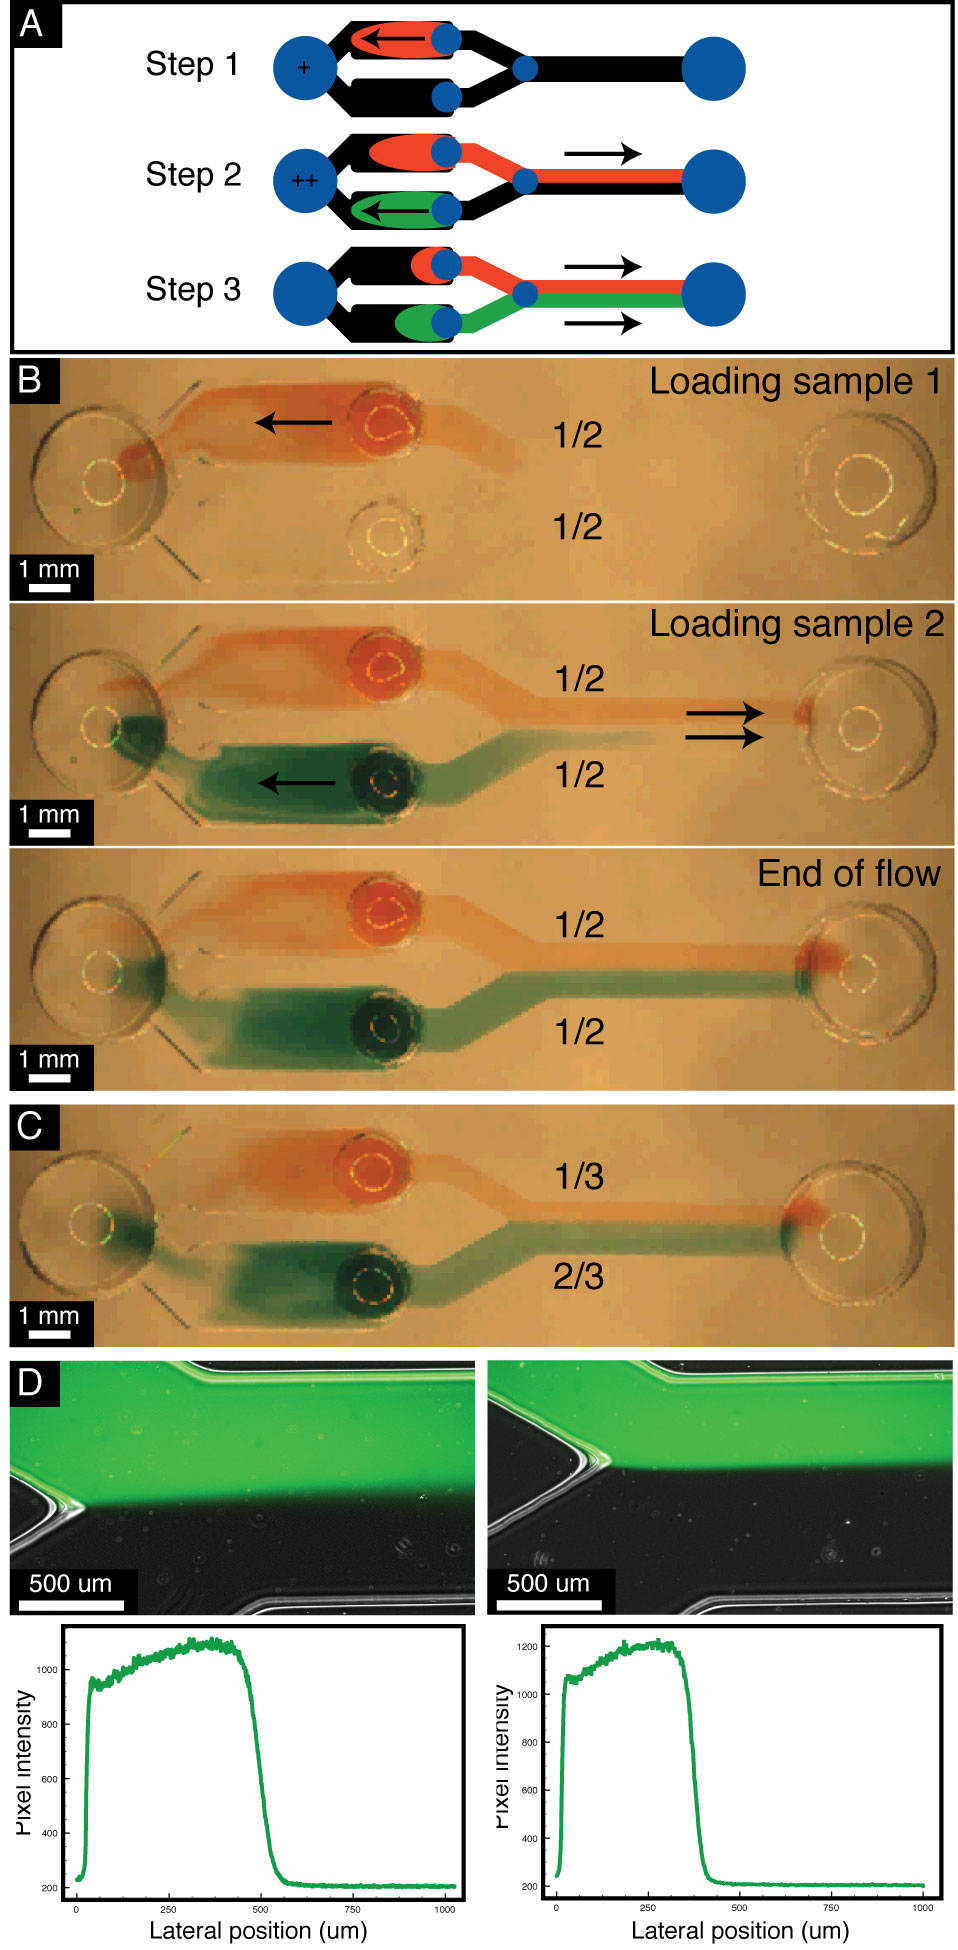
\includegraphics[width=8cm]{figure2.jpg}
  \caption{\textbf{Experimental validation of pipette-based LFP}. All sample fluids were added with a minimum of 3 seconds between each event. A. Simple three step description of the loading protocol. B. Three frames picturing a channel with equal ratio patterning at different time-points of the process. C. Image at the end of the flow in a channel designed to split the culture channel into 1/3 and 2/3 sections. D. Fluorescent and bright field merged images of Alexa488 dye flow in the 1/2-1/2 patterning device (left) amd the 1/3-2/3 device (right) and a the respective cross section fluorescent intensity profile. }
  \label{fig:experimental1}
\end{figure}

\subsection{Analysis of Each Device Component}

Analytical and numerical modeling have been performed to better understand the contribution of the different components of the microfluidic device. In order to adapt the use of this method to other applications, each component and the design considerations required for its proper function are discussed. \\

{\bf Surface tension and port capacitors.} The fluid-air interface formed by a port can be used as a capacitor in a fluidic circuit, having a pressure-volume relationship. The surface tension-generated pressure, $P_{port}$, in a droplet of curvature $R_{curv}$, at each port acts as a capacitor of fluid according to the Laplace relationship shown in Eq \ref{eq:laplace} where $\gamma$ is the surface tension of the fluid. The volume of liquid, $V$, contained in a port, can also be linked to the radius of curvature using Eq \ref{eq:volumeSphericalCap}. Eq \ref{eq:laplace} and Eq \ref{eq:volumeSphericalCap} establish a pressure-volume relationship that defines the capacitor. For instance, a large port will be able to contain a large volume of fluid and will act as a weak capacitor, whereas a small port will act a stiffer capacitor generating large pressures when fluid is added. 

\begin{equation}
P_{port} = \frac{2\gamma}{R_{curv}}
\label{eq:laplace}
\end{equation}

\begin{equation}
V = \frac{\pi}{3} (2R_{curv}^{3} - (R_{curv}^{2} - a^{2})^{1/2} (2R_{curv}^{2} - a^{2}) )
\label{eq:volumeSphericalCap}
\end{equation}

As seen in Fig \ref{fig:scematic}B, small ports (low-volume, stiff capacitors) are used for the loading ports of the device while large ports (high-volume, weak capacitors) are used to link the inputs and act as low pressure points for the fluidic circuit. Each large port is made big enough to absorb the whole amount of liquid that will be inserted for patterning. The loading ports are made small enough to quickly drive fluid to the capacitor and reduce synchronization times (Fig \ref{fig:modeling}). \\

\begin{figure}[!t]
\centering
  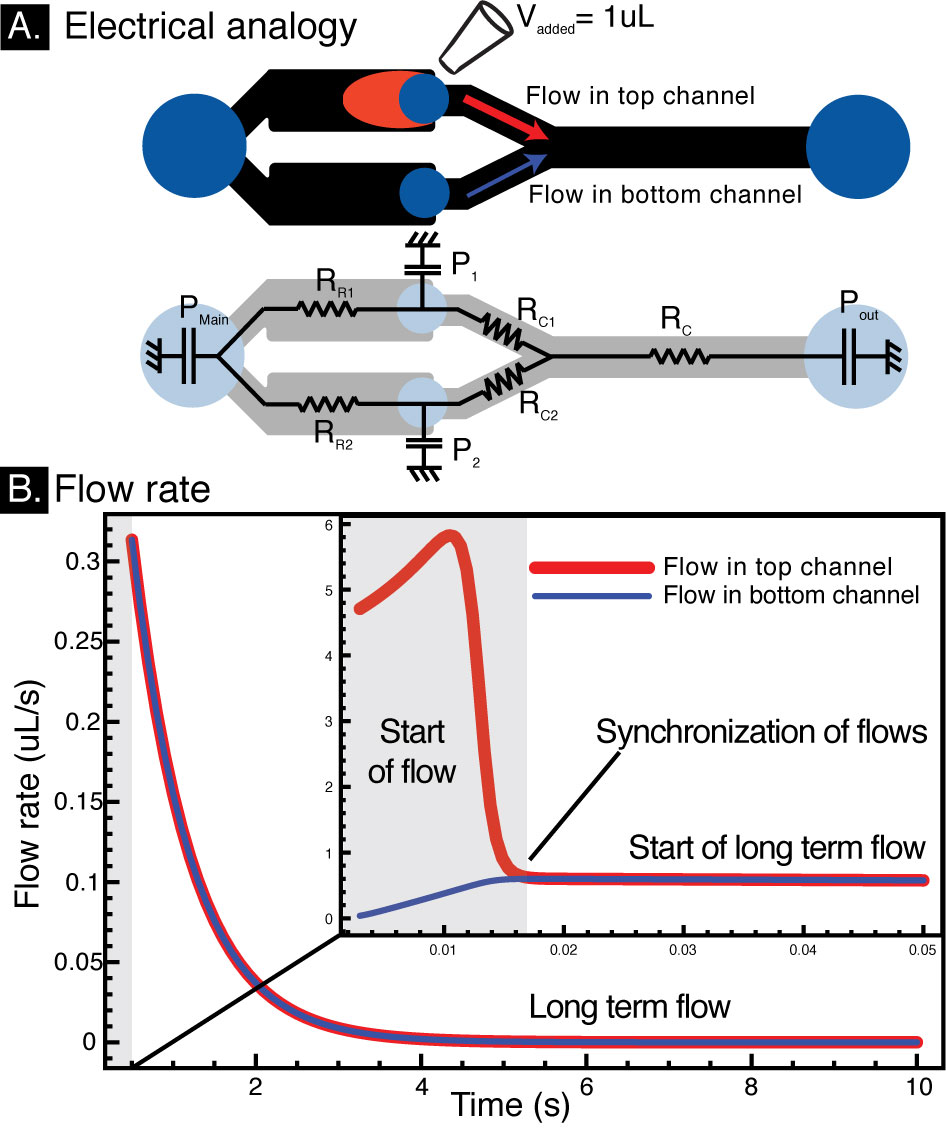
\includegraphics[width=8cm]{figure3.jpg}
  \caption{\textbf{Flux capacitor operation}. A. Electrical circuit analogy used for the numerical simulation. The different passive pumping ports can be modeled as capacitors. B. Flow rate vs. time in the each branches of the Y channel. Port pressures begin at different values, resulting in imbalanced flow rates. Within 15 ms port pressures equilibrate, leading to synchronization of the flows in both branches of the ``Y''. }
  \label{fig:modeling}
\end{figure}

{\bf Synchronization of the flow.} The experimental results of Fig \ref{fig:experimental1} show that laminar flow patterning is maintained throughout pumping. However, a short-lived disturbance of the flow pattern occurs upon each addition of fluid to an input port, which is difficult to identify in the images. The disturbance results from the short amount of time it takes for the capacitor to be charged. Simulations performed to characterize the transient flow profile in each branch of the Y-channel after adding a single droplet of 1.0 $\mu$ L in one of the input ports show that synchronization of the flows occurs in 15 ms (Fig \ref{fig:modeling}B). During the rest of the flow (4 s) the flows in both branches of the Y channel match. An additional drop can be applied to any port at anytime (before or after the flow stops), causing the process of synchronization described here to be repeated. Shorter synchronization times minimize the time that flows are imbalanced and can be achieved by reducing the radius of the sample loading port, decreasing the volume being loaded, and reducing the resistance of the reservoir channels. \\

{\bf Reservoir channel design.} The reservoir channels keep samples from mixing in the capacitor port. If the samples are allowed to reach the capacitor, samples might mix or possibly travel down an alternate branch of the device. Thus, the reservoir channels must be able to accommodate the entire sample volume. Based on previous characterizations of flow in rectangular channels, the amount of fluid needed to go beyond the end of the reservoir, $V_{overfill}$, is at most 0.48 times the volume of the reservoir due to parabolic flow profiles (Eq \ref{eq:volumeError2}) \cite{Warrick:2007lq}. Using this piece of information, the length of the reservoir channel can be designed appropriately. \\

\begin{equation}
V_{overfill} \ge 0.48 \, V_{channel}
\label{eq:volumeError2}
\end{equation}

{\bf Y channel design.} The ratio of flow down each branch of the Y-channel after synchronization, $Q_{1}/Q_{2}$, is proportional to the ratio of the resistances of each branch, $R_{C2}/R_{C1}$. Although the primary function of the branches is to determine where the interface between the flows will be patterned, they must also be designed to allow enough time for synchronization (Fig \ref{fig:modeling}B). As mentioned previously, the Y-channel has a significantly higher resistance than the reservoirs such that when fluid is added to a loading port, most of the fluid travels directly to the capacitor port, charging it with fluid. Channel dimensions can be reduced to pattern narrower regions of interest (50-100 $\mu$m) and would result in longer pumping times. The pumping mechanism can be scaled to increase pumping velocities to avoid cell settling during patterning.\\

%{\bf Sample loading.} The timing of the loading no longer influences patterning but can affect how much sample is left in each reservoir channel after patterning. In the case of symmetric patterning, after the first sample is loaded and comes to rest, half of the sample will remain in the reservoir channel. After loading the second sample in the other port, the remainder of the first sample will be pushed out of its reservoir channel and half of the second sample will remain in its reservoir. Alternatively, if the loading of the first and second sample had been perfectly synchronized, none of either sample would remain in the reservoir channels. %Both cases result in symmetric patterning but have different amounts of sample left over in the reservoir channels. Furthermore, this illustrates that a limited amount of time may still be required between sample loading if sedimentation of particles in the sample fluid is an issue of importance. 

\subsection{Patterning of More Than Two Streams}
\begin{figure}[!t]
\centering
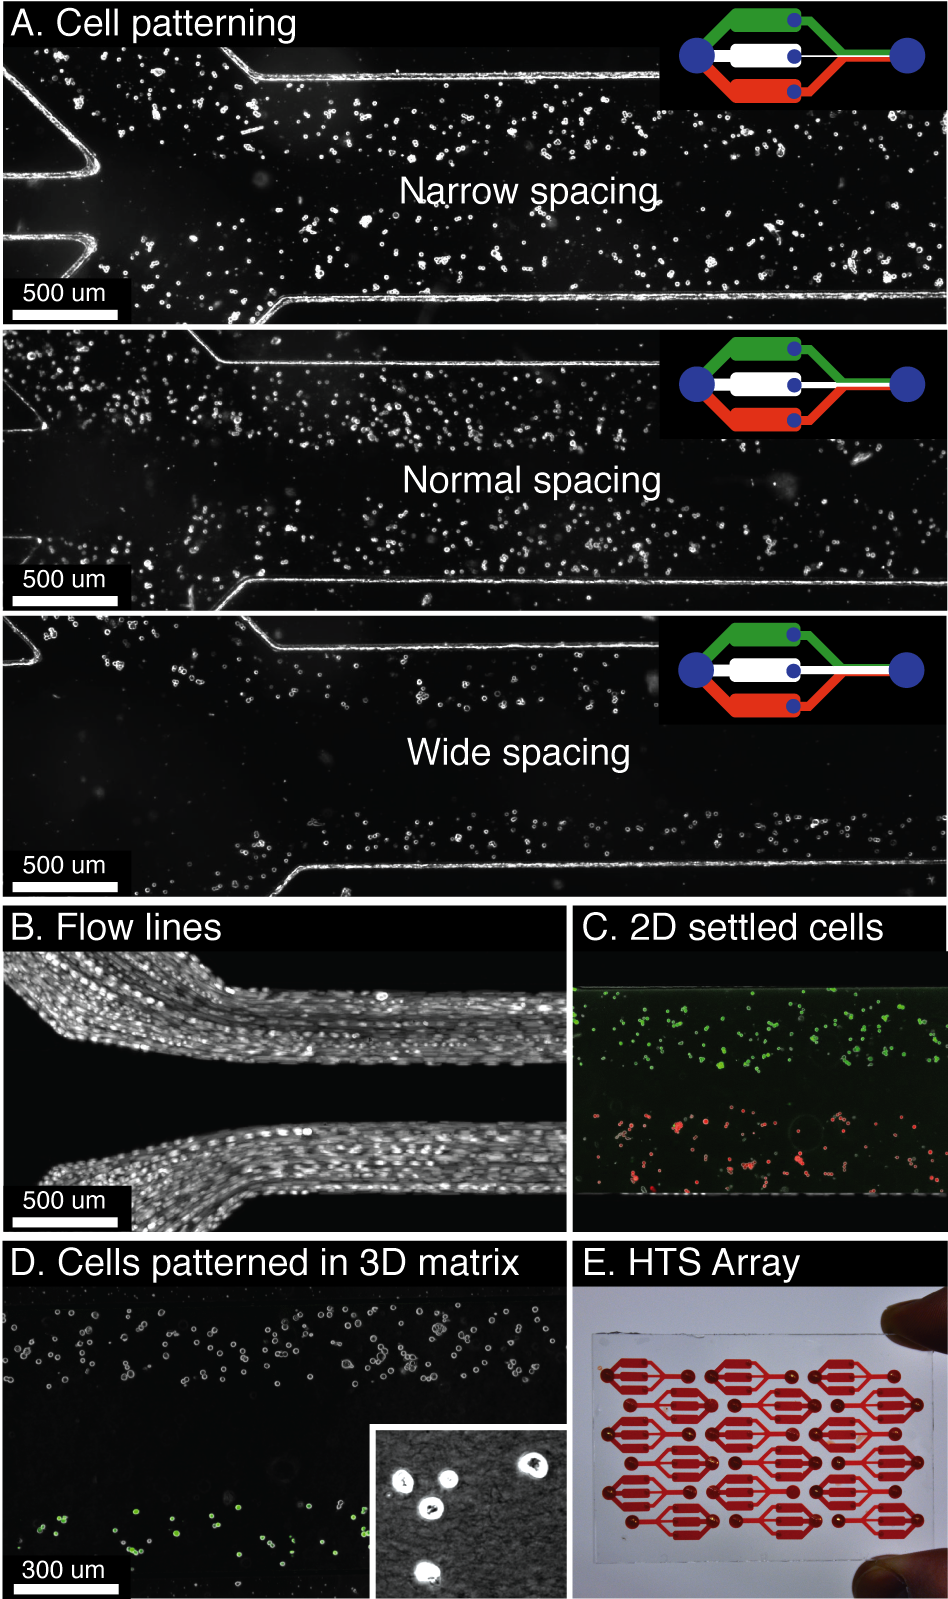
\includegraphics[width=8cm]{figure4.png}
  \caption{\textbf{Laminar flow patterning demonstrations}. A. Demonstration of a wound-healing/migration assay with variable spacing between the two cell populations. The upper right diagram represents the microfluidic device geometry. B. Multiple contrast enhanced movie-frames superimposed to illustrate the flow paths of cells being patterned in the wound-healing\slash migration device. C. RFP and GFP MCF7 cells patterned into a three-flow device. D. Osteoblasts (MC3T3-E1) and prostate cancer cells (LNCaP) are patterned within in a collagen matrix. The inset shows collagen fibers formed after polymerization using phase contrast imaging. E. Illustration of the arraying ability of the method for high-throughput screening (HTS) applications. All images  were taken within 15 min of seeding.} 
  \label{fig:experimental2}
\end{figure}

Fig \ref{fig:experimental2} illustrates the ability to scale the technique to incorporate more than two streams for 2-D or 3-D culture as well as for increased throughput and screening applications. Cell suspensions of MCF7 cells transfected with either GFP or RFP were patterned a set distance apart using a third stream of PBS directed down the center of the channel. In each case, only the width of the center branch was varied to produce a narrow (150 $\mu$m), medium (250 $\mu$m), and wide (600 $\mu$m) spacing (Fig \ref{fig:experimental2}A). Fig \ref{fig:experimental2}B is the superposition of multiple movie frames taken using phase contrast in order to illustrate the path of each cell in suspension as it travels. Fig \ref{fig:experimental2}C shows the final result of patterning using a false-colored overlay of the fluorescent images with an enhanced phase contrast image. Fig \ref{fig:experimental2}D demonstrates the ability to pattern cells in 3-D matrices such as collagen. As shown in Fig \ref{fig:experimental2}E, the individually addressable devices can be arrayed to enable inclusion of multiple experimental conditions on a single chip.

\subsection{Patterning for Cell-Based Assays}

%\subsection*{Discussion and Demonstration of Potential Applications}

The pipette-based strategy makes the method significantly more accessible to biologists by eliminating the need for syringes, tubes, and fluidic connections. The method is also more appropriate and robust for cell-based applications than other pipette-based methods which require the use of surface treatments and surfactants in the fluid to make patterning predictable \cite{Kim:2005fk}. As with other pipette-based methods, flow is transient and best-suited for applications where only a short period of flow is needed to establish the desired pattern, such as transient gradient generation, co-culture assays, wound-healing assays, and other particle patterning applications in 2-D or 3-D. Fig \ref{fig:cocultureData} illustrates the ability to use this method with cells to perform wound healing and co-culture assays.

%{\bf Generating Gradients.} Gradient generation is one of the most popular applications of LFP, and is used to study gradient sensing, chemotaxis and stem cell differentiation. Using passive pumping methods, transient gradients of factors are readily achievable by flowing two different media in the Y-channel (Fig. \ref{fig:gradient}). The gradient is initially steep at the boundary between the different fluids and eventually equilibrates. The time over which this occurs is given by Eq \ref{equ:transientGradient} with $D$ being the diffusion coefficient and  $L_{W}$ being the width of the channel. Longer term gradients can be achieved by subsequent applications of new drops at the loading ports to reset the gradient or through the use of a different pumping strategies. Nevertheless, transient gradients can be sufficient to study short term phenomena, such as the chemotaxis of rapidly migrating cells such as leukoctyes \cite{Berthier:2010uq}.

%\begin{equation}
%t = \frac{ L_{W}^{2} }{2D}
%\label{equ:transientGradient}
%\end{equation}

%\begin{figure}[!t]
%\centering
%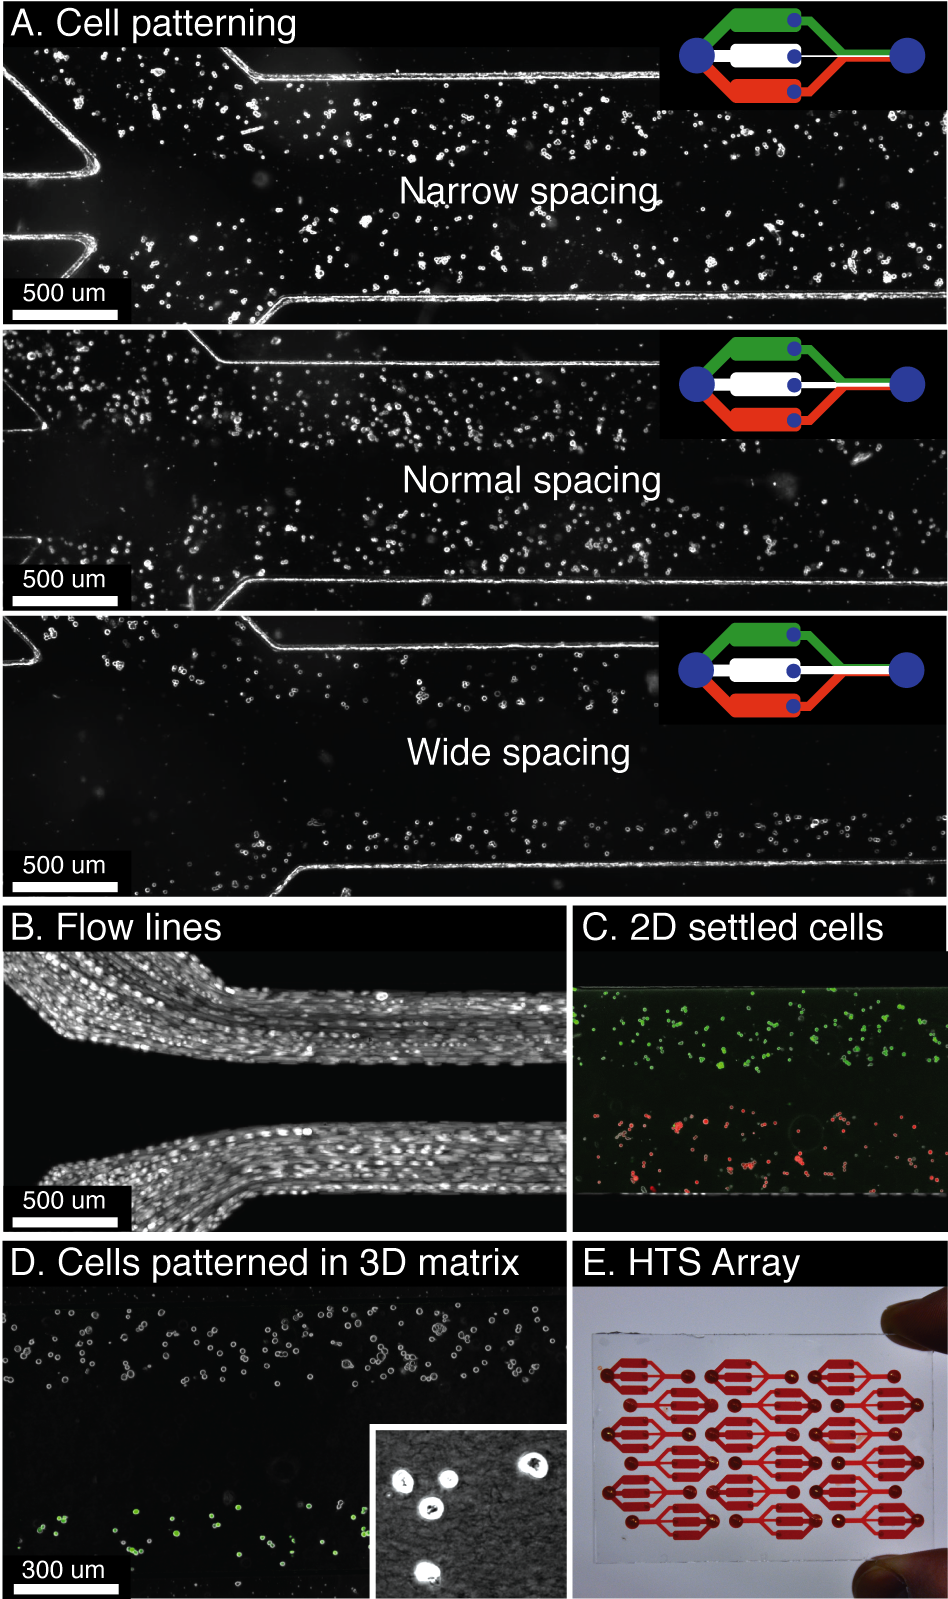
\includegraphics[width=8cm]{figure4.jpg}
%  \caption{Creation of a transient gradient using LFP of two different solutions.  }
%  \label{fig:gradient}
%\end{figure}



%A three-flow LFP devices (Fig \ref{fig:experimental2}) can be used to repeatably establish a gap between two cell populations for the study of soluble factor effects in co-culture and wound-healing\slash migration assays. The primary difference between these two types of assays is whether or not cells are allowed to migrate and close the gap. In a wound-healing/migration assay, closing of the gap is desired but can also result in cell-cell contact. In contrast, cell-cell contact can confound results in co-culture assays aimed at isolating soluble factor effects making it desirable to avoid cell migration in the region between the populations. This patterning method is flexible and can be used in conjunction with surface treatments or other culture channel geometries to avoid gap closure and prolong observation of soluble factor interactions. Although LFP has been used for these types of assays in the past, the method described here makes it significantly more accessible to a broader audience. In order to highlight some of the advantages of LFP for those that might now employ it in their application, a device for studying soluble factor interactions is demonstrated and compared to other more common methods of segregating cells, such as the use of constrictions or barriers.

The patterning technique was used with a lung epithelial cell line (BEAS-2B) to illustrate the potential for performing wound healing assays. Dotted lines show the initial patterning location and the advance of the cells onto the blank substrate in the center. Groups of cells form protrusions via collective migration instead of each cell migrating independently to advance the front uniformly (Fig \ref{fig:cocultureData}A, Day 2, white arrow). Fig \ref{fig:cocultureData}B illustrates the same patterning method with two different cell types, MC3T3-E1 and LNCaP, to demonstrate a directed cell migration or invasion assay. Given the channels are individually addressable without the use of valves or other microfluidic components, appropriate controls can be easily performed on the same array (i.e. blank+A, A+A, B+B, and blank+B). Similarly, different treatments can be applied to each channel at different time-points. A subtle, but important, capability of this method is the ability to change the cell ratio (i.e. 2 x A + B, or A + 3 x B) using different flow ratios (see Fig \ref{fig:experimental1}) while maintaining a constant surface cell density -- something that cannot be done in standard transwell assays \cite{Domenech:2009jt}. This ability can be crucial for controlling the confounding effects of density dependent cell behavior seen in many \emph{in vitro} models of cell signaling.
\begin{figure}[!t]
\centering
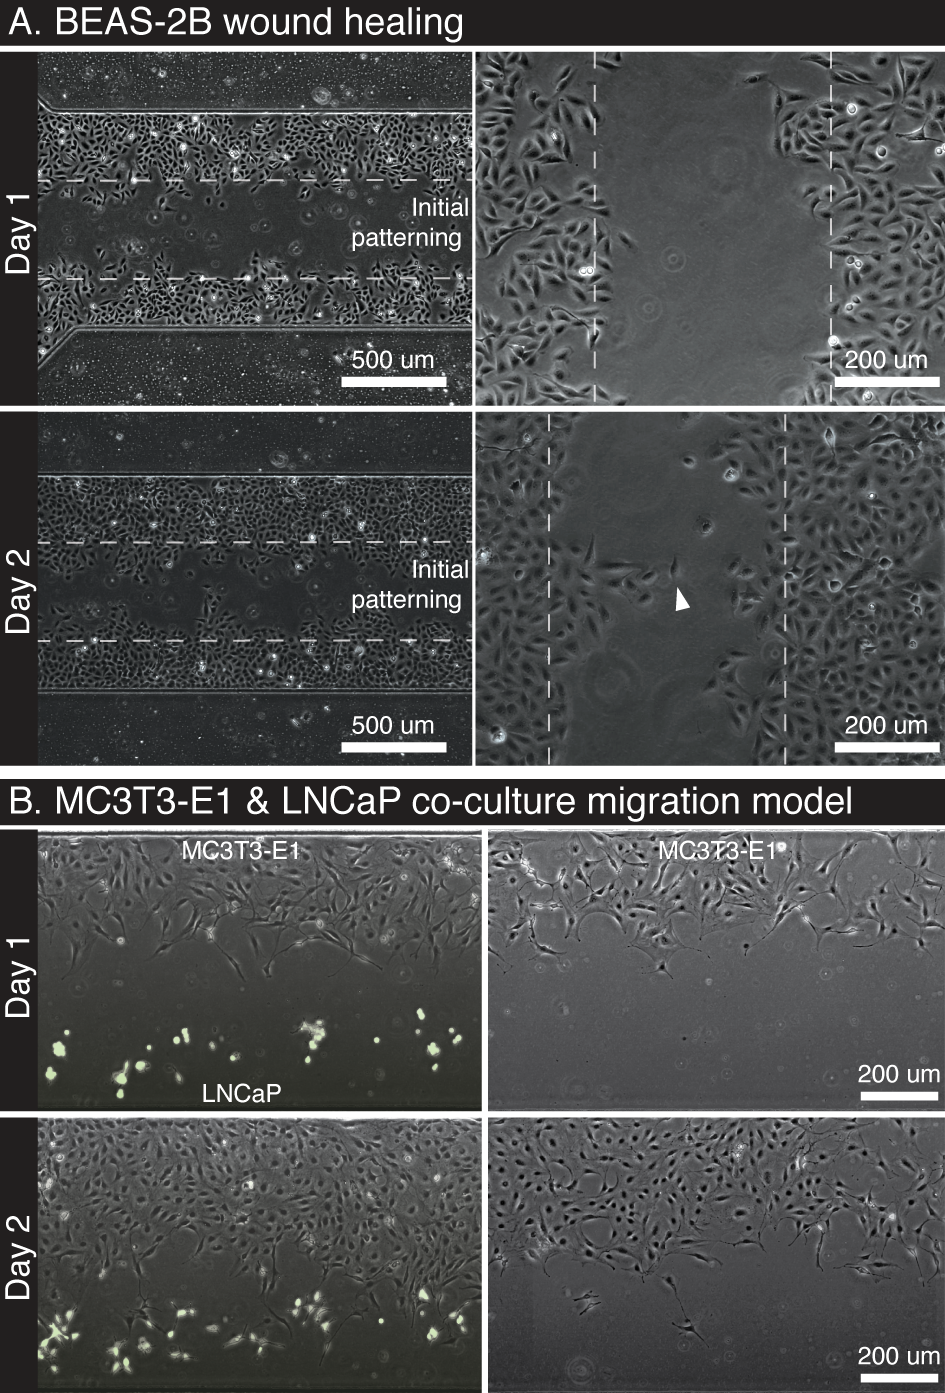
\includegraphics[width=3.2in]{figure5.png}
\caption{\textbf{Wound and migration assays}. A. Wound healing assay. BEAS-2B cells initially patterned with a defined gap and observed using phase-contrast over the course of 3 days. B. Migration assay. MC3T3-E1 and LNCaP (GFP$^{+}$, green) cells initially patterned with a gap to observe migration. A no-LNCaP control is provided within the same microchannel array as a control.}
\label{fig:cocultureData}
\end{figure}

This pipette-based approach offers multiple specific advantages for cell-based assays in addition to increased accessibility. Each channel is individually addressable allowing any number of fluids and cells suspensions to be loaded into a each channel of an array at any time without valving or changing fluidic connections. Arrays of the pipette-based devices can be addressed using liquid handling automation to increase throughput. Soft-lithography can be used to tailor the device geometry to change the ratio of one cell-type to another without changing the surface cell density. The distance between the groups of cells can be tuned to modulate soluble factor signaling to study soluble factor sensitivity. Additional branches can easily be added to create more complex co-culture assays containing more than two cell types. The device also supports the culture of cells in small volumes to enable more rapid accumulation of factors, a characteristic which has shown to improve co-culture sensitivity \cite{Domenech:2009jt}. Taken, together, the method offers significant advantages that increase the flexibility of the method and can broaden the use of LFP in cell-based assays.

%\begin{figure}[!t]
%\centering
%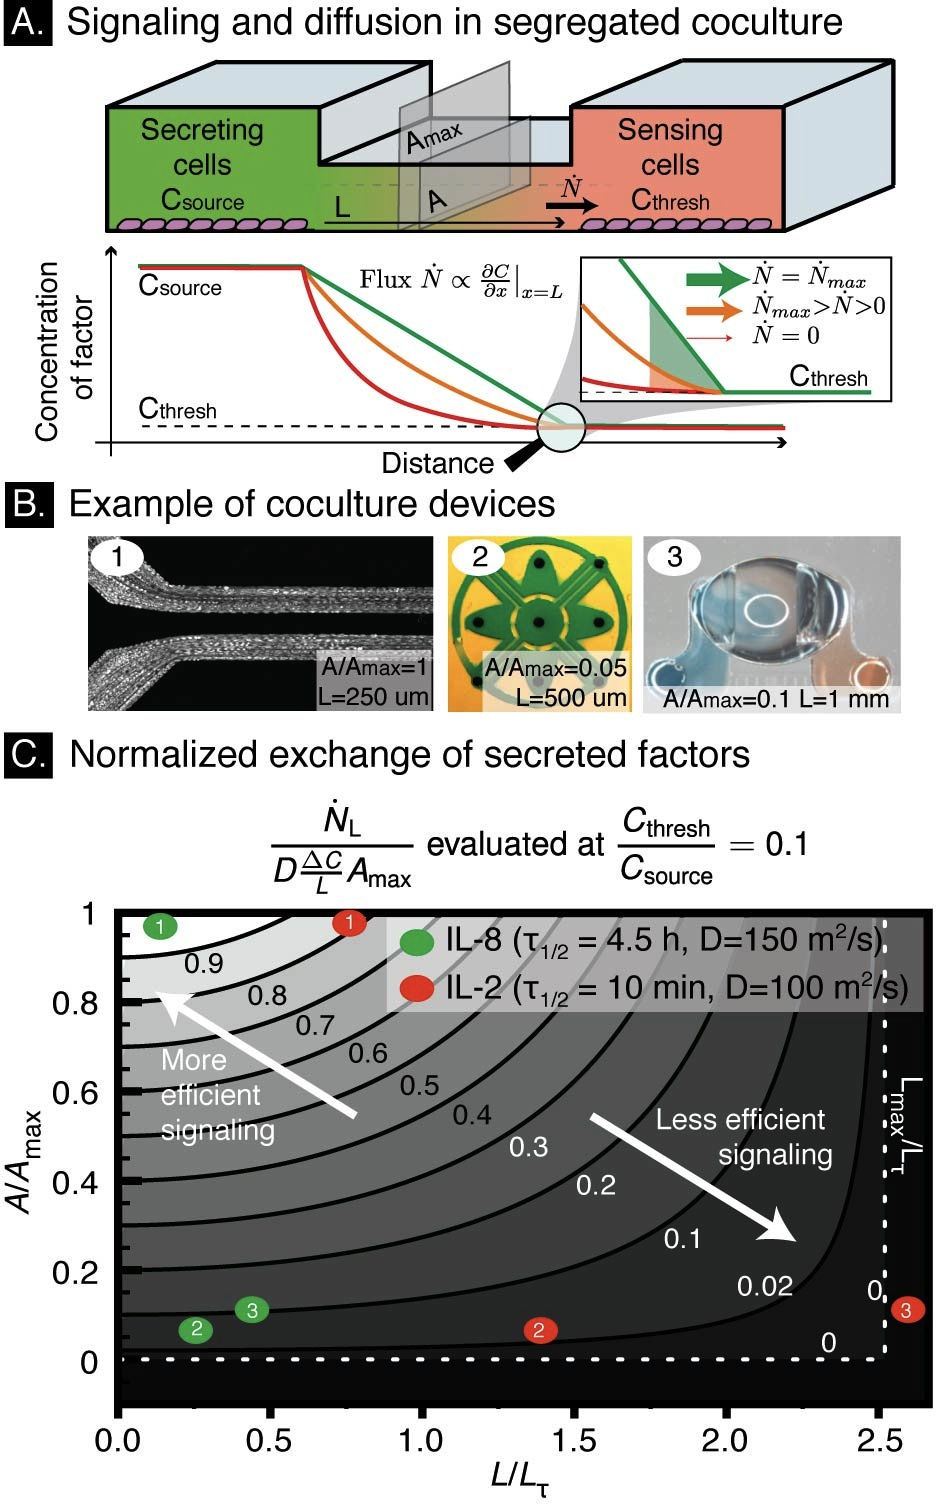
\includegraphics[width=3.2in]{figure6.jpg}
%\caption{Typical approaches for studying cell co-culture in a microchannel while keeping the cell cultures seperated. Laminar flow patterning provides the highest signaling ability as it maximizes diffusional exchange. Segregated co-culture provides simple sequential loading ability, though the flow-restricting constriction acts to limit signaling flux \cite{Domenech:2009jt}. Gel separated co-culture approach allows simple loading of the cell sample and usually higher signaling flux than segregated co-culture however fabrication and setup are more complex \cite{Sudo:2009fk}.}
%\label{fig:cocultureSchematic}
%\end{figure}

%Given the limited use of LFP for coculture and that many different devices and methods exist to perform segregated coculture, a qualitative analysis of diffusion between two cell populations is used to illustrate how LFP can be leveraged to improve soluble factor exchange. In a coculture assay, the groups of cells are typically separated by a gap through which factors must diffuse to initiate signaling. This basic scenario is illustrated in Fig \ref{fig:cocultureSchematic}. The three critical parameters that determine the efficacy of signaling between the populations are; $L$, the distance between the groups of cells; $D$, the diffusion coefficient; and $A$ the cross-sectional area through which the transport must occur. Using Fick's first law of diffusion, we can see that using constrictions to aid cell patterning acts to reduce the cross-sectional area for diffusion and thus diminish the rate of diffusive transport, $\dot{N}$ (Eq \ref{equ:ficks}, Fig. \ref{fig:cocultureSchematic}B). 
%\begin{equation}
%\dot{N} = D\,\frac{\partial C}{\partial x} A
%\label{equ:ficks}
%\end{equation}
%A similar effect is seen when the diffusion coefficient in the gap between the cells is lowered\cite{Domenech:2009jt}, for example with the use of gels or membranes as cell barriers \cite{Sudo:2009fk} (Fig \ref{fig:cocultureSchematic}C). The $\partial C/\partial x$ term suggests that culturing the cells in close proximity (\emph{i.e.}, by reducing $L$), helps to improve transport. Pipette-based LFP provides a way to implement coculture, wound-healing, and migration assays while avoiding the use of constrictions or barriers and enabling precise control of the distance between the each population to promote soluble factor signaling.

\section{Conclusions}

While LFP is an attractive method for studying cell migration, soluble factor signaling, and other biological phenomena, it has not been readily available for robust every-day-use in biology laboratories. The passive LFP method described here allows samples to be loaded at any time and in any order using only a pipette without depending on the use of syringes, tubes, fluidic connections, surface treatments, or surfactants. This advance enables the design and creation of practical assays that can leverage advantages of LFP to study soluble factor signaling and are amendable to use in biology labs. Furthermore, the synchronization method described here is compatible with patterning and in-situ polymerization of cell-laden hydrogels such as collagen or matrigel. These are increasingly gaining momentum as being central to the study of cell migration/invasion in three-dimensional matrices as they offer more physiologically relevant environments \cite{Sung:2010fk}.

\section{Acknowledgements}
David J. Beebe has an ownership interest in Bellbrook Labs LLC, which has licensed technology reported in this publication. The developments reported were accomplished through funding from the following grants: NIH-NCI R33 CA137673, DOD PCRP Idea (W81XWH-09-1-0192), Korea Research Foundation Grant (KRF-2008-220-D00133), a traineeship from the National Library of Medicine (5T15LM007359, J. Warrick) and a doctoral fellowship from the Morgridge Institute for Research (E. Berthier). We wish to thank Sameer Mathur for providing the BEAS-2B cells.
\chapter{Components: `The Concentrator' for Rare Cell Populations}
\label{Chap:Concentrator}

\section{Preface}
Contents of this chapter are taken primarily from \cite{Warrick:2010fk}.

\section{Introduction}
In cell-based assays, the number of cells per unit volume is often a critical parameter and is typically controlled using the process of centrifugation and resuspension. However, if the number of cells is small enough, the resuspension volume needed to achieve a desired density can become much less than 50 \textmu L posing a significant challenge to downstream use.  In practice, this volume limits how dense a cell suspension can be made using centrifugation. Thus, in rare cell applications (\eg , cells isolated using flow cytometry, circulating tumor cells, or primary samples from small animals) centrifugation can be inadequate to achieve appropriate cell densities for study. Further, it is difficult to work with such small volumes - bubbles can interfere with cell handling and resuspension, cells may be lost while aspirating the supernatant, or there may not be enough cells to form a proper pellet. 

Microscale devices can help address this and other challenges of working with rare cells. For example, there is an inherent reduction in the number of cells needed to perform cell-based assays compared to macroscale alternatives, thus increasing the number of experiments that can be run with a given sample. It has also been observed that reducing the scale of an assay can also increase its sensitivity and functionality\cite{Chen:2005ys,Walker:2004gs,Breslauer:2006nx,Domenech:2009jt}.  However, the limitations of centrifugation become even more prevalent in microscale applications as they generally require high cell suspension densities. In microculture, the ratio of the number of cells to volume of culture media (cell:volume ratio) after seeding is typically 4-10 times greater compared to culture flasks or well plates\cite{Paguirigan:2009bh}. As a result, approximately $\sim$50,000\footnote{This limit is calculated based on a seeding density of 250 cells/mm$^{2}$ for culture in a microchannel with a height of 250 \textmu m (\ie , a density of 1000 cells/\textmu L). It is also assumed that the original sample is centrifuged to a minimum volume of 50 \textmu L to avoid aspiration of any concentrated cells. The limit is specific to the application.\label{fn:thresh}} cells must be acquired to reach appropriate culture densities using centrifugation. Acheiving appropriate densities is particularly important in primary cell culture applications where cell density and\slash or cell number can dictate the outcome of an experiment\cite{Domenech:2009jt}.

Specialized alternatives to centrifugation exist for microculture applications when cell numbers are below this threshold; however, they typically use a filtering or capture methodology that involves the use of physical impediments\cite{Zheng:2007fk,Kuo:2010uq}, electric charge\cite{Gascoyne:2009kx,Sankaran:2008vn,Hsiung08}, or surfaces functionalized with recognizable biomolecules, such as nucleic acids\cite{Douglas:2009dq,Hsiao:2009zr,Xu:2009ly} and antibodies\cite{Dharmasiri:2009ys,Plouffe:2009oq,Sherman:2010cr,Russom08} -- all of which can alter cell physiology. For example, recent work has focused on designing size-based mechanical filters that reduce issues of cellular deformation and lysis \cite{Kuo:2010uq}. Microfluidic devices offer gentle alternatives to these methods, often utilizing changes in channel dimension\cite{Mohamed:2009nx,Jain:2009tg}, inertial focusing\cite{Kuntaegowdanahalli:2009kl,Di-Carlo:2008ve}, or nanostructures (\eg , pillars or cups) to separate target cells\cite{Hosokawa:2009bh,Green:2009qf}.

\begin{figure*}[!t]
\centering
\begin{tabular}{@{}c@{}c@{}}
\multicolumn{1}{l}{A)} & \multicolumn{1}{l}{B)} \cr
\hspace{0.5cm}\includegraphics[height=1.8in]{RadialConcentrator_SchematicFinal.pdf} &
\hspace{0.5cm}\includegraphics[height=1.8in]{RadialConcentratorMovieSequence2.pdf}
\end{tabular}
\caption{\textbf{Design and operation of a microfluidic device for gentle cell collection and treatment}. a) Labeled isometric view of Design II along with cross-section views of both Design I and II. b) Images from a movie capture showing LNCaP cells (white spots in the phase contrast images) being deposited in the collection region of Design II using a single 15 \textmu L droplet of dense cell suspension. On the right, a conceptual representation of cell trajectories through the device illustrates the potential for cells to pass through the collection region. Cells that enter on higher streamlines have a greater chance of passing through.}
\label{fig:device}
\end{figure*}

We present a microfluidic method for simultaneously concentrating a cell suspension and depositing the cells into a simple microfluidic channel that can be used for a wide variety of downstream assays, including cell culture and biochemical analyses. This method is intended for concentrating cells that have been previously isolated through other techniques such as density gradient centrifugation (\eg , Ficoll-Paque or OncoQuick) or negative selection with magnetic beads. An important advantage of this microfluidic method is that the cells are exposed to minimal amounts of shear while avoiding the use of size-based mechanical filters, electric charge, and adhesive surfaces in an attempt to minimize perturbation of the cells and the microenvironment. Further, this method provides a way to subsequently culture and gently treat those cells, providing the same functionality as a typical microchannel. The method is widely applicable, addresses an important challenge to the study of rare cells (\ie , concentration), and provides a means to interface rare cell samples with microscale devices for advanced analysis of cellular function.

Specifically, we plan to use this method to enable microscale studies of circulating tumor cell (CTC) function. CTCs are tumor cells found in the blood of cancer patients and have emerged as potential prognosticators of metastasis; however, only hundreds or thousands of these cells can be obtained per blood draw, making them difficult to study\cite{Okegawa09}. The method presented here could be used to promote CTC survival and growth by encouraging cell-cell signaling through higher cell:volume ratios. The additional concentration provided by the device lowers the number of CTCs that need to be isolated from a patient in order to achieve the desired culture densities. Higher numbers of CTCs per device also increases the robustness of biochemical readouts and facilitates microscopy endpoints by confining the target cells to a small, well-defined region-of-interest.

\section{Experimental}

\subsection{Device Design}

The microfluidic device collects cells by allowing them to gently settle into a collection region (Fig \ref{fig:device}). The cells accumulate in the collection region thereby increasing the concentration of cells per unit volume. A droplet of cell suspension is dispensed at the input port using a pipette. The cell suspension is then driven radially outward through the device via surface tension in the droplet\cite{Berthier:2007mi,Chen:2009df}. Cells are carried from the input via small, constrictive transport channels with relatively rapid velocity and high resistance compared to the expansive, slow-velocity collection region. The more rapid flow of the transport channels keeps cells from adhering to the substrate while the low-velocity collection region allows cells to settle out of the flow and interact with the substrate. Non-specific interaction between the cells and a tissue culture treated polystyrene substrate is able to withstand the small amount of shear stress present and keeps the cells from passing through the collection region while fluid depleted of cells continues to pass through the device\footnote{It should be noted that the interactions between cells and substrates are dynamic and unique to the cell type and conditions of the microenvironment. The cell collection method demonstrated here relies on non-specific interactions in order to reduce variability in retention from cell-type to cell-type as compared to the use of specific adhesion ligands; this method further avoids any difficulty associated with the creation of such specialized surfaces. However, this microfluidic method does not preclude modification of the substrate to enhance retention of a specific cell type.}. Subsequent droplets placed at the input port of the device can be used to gently treat or wash collected cells.

The fluid velocities in the transport channels and collection region are very different due to a difference in the cross-sectional area perpendicular to flow. In this case, the flow is traveling radially outward from the input port to the outer ring. Given a volumetric flow rate $Q$, the average flow velocity, $V$, and the cross-sectional area perpendicular to flow, $A$, within a particular region of a device are related by $V=Q/A$. The total flow rate, $Q$, within the transport channels is the same as in the collection region, only the cross-sectional areas differ, leading to dramatic differences in velocity within each region. Based on channel dimensions, average fluid velocity drops as it enters the collection region by a factor of 1/211 in the first design and by 1/114 in the second design promoting cell collection.

Fig \ref{fig:device} shows two embodiments of this methodology. Both designs are radial in nature. The major difference lies in the dimensions of the collection region. Data presented here will be used to elucidate the effects of collection region geometry on the ability of the device to collect cells in terms of overall throughput and percentage of cells that avoid collection. Although the influence of the transport channels, collection region, and passive pumping all interact with each other to create a balanced system for effective collection of cells, considerations for the implementation of each component are discussed in separate subsections.

\subsubsection{Transport Channels} \label{sec:transport}

The transport channels dictate the overall flow rate through the device, $Q$, as they account for almost all of the pressure drop between the input and output port (see Appendix \ref{App:Concentrator}). As a result of the high resistance and radial design, the flow through each transport channel is within 0.55\% of each other (see design simulation data ESI). In terms of device operation, this means that the high resistance of the transport channels causes fluid to be delivered uniformly across the collection region for even cell seeding, treatments, and washing. Also, given that the overall flow rate of the device must remain low enough to promote cell settling in the collection region, the radial design optimizes the number of transport channels that can symmetrically draw fluid away from the input port to maximize throughput and minimize cell settling before entry into the transport channels.

\subsubsection{Collection Region}

Appropriate cell settling in the collection region influences the efficiency of the device in terms of number of cells lost to the device output. The main parameters that dictate whether cells settle to the surface or not are the flow velocity, $v_{f}$ [mm/s]; the cell settling rate, $v_{c}$ [mm/s]; the height of the collection region $h$; and the length of the collection region, $l$. These parameters affect how much time it takes to pass through the collection region, also called the residence time or $t_{res}$, and how long it takes a cell to settle, $t_{set}$. The residence time can be estimated as $t_{res} \approx l/v_{f}$ whereas the characteristic settling time is defined here as $t_{res}\approx h/v_{set}$. Cells that do not have sufficient time to settle to the surface (\ie , $t_{res} < t_{set}$) will pass through and be lost to the outer ring. The actual residence and settling times of a cell depend upon its position in the flow streams of the device as it enters the collection region.

\subsubsection{Passive Pumping}\label{sec:pp}

The parameters of passive pumping offer a way to tune flow rates without altering any device dimensions. Passive pumping depends primarily upon three factors: the surface tension of the fluid, the wetted diameter of the input droplet, and the initial volume of the input droplet\cite{Berthier:2007mi,Chen:2009df}. It is difficult to control surface tension in the context of cell culture so discussion will be limited to the remaining two parameters. The internal pressure, $\Delta P$, of a droplet used to drive passive pumping is given by the Young-Laplace equation shown in Eq \ref{equ:laplace}, where $r$ is the radius of curvature for the droplet and $\gamma$ is the surface tension. The maximum pressure, $\Delta P_{max}$, that can be developed using passive pumping is directly related to the radius of the wetted area of the droplet at the input port, $r_{w}$, by the equation $\Delta P_{max}=2\gamma / r_{w}$. In other words, maximum pressure occurs when the droplet is a hemisphere and has lower pressures at greater or lesser volumes. Thus, the maximum pressure and resulting fluid velocity in the collection region can be controlled by the wetted diameter or regulated by the volume of fluid placed at the input.

\begin{equation}\label{equ:laplace}
\Delta P = 2 \gamma / r
\end{equation}

\subsection{Device Fabrication and Preparation}

Devices were made of polydimethylsiloxane (PDMS, Sylgard 184, Dow Corning). Molds for the PDMS devices were made using soft lithography techniques that have been described previously\cite{Duffy:1998vj}. Fig \ref{fig:device} contains a labeled schematic with cross sections of the two device designs. Design I uses a collection region that is 750 \textmu m wide $\times$ 650 \textmu m tall compared to 1250 \textmu m $\times$ 350 \textmu m for Design II. The outer rings for both devices are 750 \textmu m wide with a centerline diameter of 12.5 mm. The heights of the outer rings match the heights of the respective collection regions. Both designs have transport channels that are 29 \textmu m high and 100 \textmu m wide. The ports have a radius of 1 mm while the centerline of the collection ring has a diameter of 7.5 mm. A total of 50 transport channels carry fluid from the input to the output ring.

The devices were sterilized using an autoclave or by washing with ethanol for $>$ 4 hrs. The empty sterilized devices were placed on tissue culture plastic polystyrene omni-trays (Nunc, Rochester, NY). The device is then filled with ethanol via capillary action followed immediately by $\ge$ 90 \textmu L of culture media using passive pumping. Finally, a predefined quantity of media was applied to the input port to define the wetted radius for passive pumping.

\subsection{Cell Culture}

The human lymph node carcinoma of the prostate (LNCaP) cell line used in these experiments was stably transfected with green fluorescent protein (GFP).  Cells were maintained at 37$^{\circ}$C, 5\% $CO_{2}$ in RPMI 1640 culture medium supplemented with 10\% fetal bovine serum (HyClone), 100 U/mL penicillin (Gibco), 100 \textmu g/mL streptomycin (Gibco), 10 mM HEPES buffer, 1 mM sodium pyruvate, and 25 mM glucose.  LNCaPs were counted with a hemocytometer and diluted to a final concentration of 50,000 cells/mL for each experiment.

A standard staining protocol was followed for the epithelial cell adhesion molecule (EpCAM) staining of LNCaPs within the microchannel.  Cells were first washed with PBS (3 x 15 \textmu L) and fixed with 4\% PFA in PBS (2 x 15 \textmu L) for 12 minutes.  Cells were then washed with PBS (3 x 15 \textmu L) and Blocked with 1\% BSA in PBS (3 x 15 \textmu L) for 20 minutes.  Primary antibody for EpCAM (2 x 15 \textmu L) was incubated with the cells at 4$^{\circ}$ C overnight and washed with 1\% BSA in PBS (3 x 15 \textmu L).  Cells were then treated with secondary antibody (2 x 15 \textmu L) which was incubated with the cells at 4$^{\circ}$ C overnight and washed thoroughly with 1\% BSA in PBS (6 x 15 \textmu L) and imaged.

\subsection{Fluid Modeling}

Fluid modeling was done using COMSOL Multiphysics 3.4 (Burlington, MA). All simulations are solved for steady-state conditions. Symmetry was leveraged to obtain high resolution solutions of fluid flow in the collection regions for analysis of cell settling and collection. Cell trajectories were modeled and used to calculate cell loss. Cell trajectories were approximated by solving for fluid velocity and adding an additional vertical velocity component to the solution that is equal to the cell settling velocity. The adjusted velocity solution is then used to determine the new, adjusted streamlines\slash trajectories in COMSOL. Thus, the adjusted streamlines are now considered cell trajectories. Cells were modeled as having settling velocity, $v_{c}$, of 2.7 \textmu m/s. This value is calculated assuming the cells have a radius of 6.25 \textmu m as measured from microscope images of LNCaP cells and a density of 1035.7 kg/m$^{3}$ based on measurements in the literature of another epithelial cancer cell line\cite{H:1987ij}. Octave (University of Wisconsin, Madison), an open source alternative to Matlab, was used for subsequent analysis of information output from COMSOL. Cells were considered to be `lost' if the model predicted they flowed completely through the collection region or if they settled on the substrate in a location with a shear stress greater than 0.1 dynes/cm$^{2}$\footnote{The shear threshold of 0.1 dynes/cm$^{2}$ is a round estimate based on previous papers looking at cell capture in flow-based microfluidic devices\cite{GIAVAZZI:1993ty,Myung:2010fk,Nagrath:2007bs}.}. Further information on the details of the fluid modeling are left to Appendix \ref{App:Concentrator}.

\section{Results and Discussion}

The ability of the two device designs to collect\slash concentrate cells and minimize loss of cells to the outer ring during both seeding and subsequent treatments is assessed as these have a direct impact on the efficiency and utility of the device for rare cell applications. A previous study provides analysis of a similar scenario in which cells are collected using steady flow in a parallel-plate flow chamber\cite{Munn:1994fk}. This analysis is extended here for the application of passive-pumping, which involves transient flows of discrete volumes.

\subsection{Dimensional Analysis of Cell Collection}

As mentioned earlier, the process of cell collection depends on the ratio of the time required for the cells to settle to the substrate, $t_{set}$, and the time the cells are in the collection region, also called the residence time, $t_{res}$. As the value of $t_{set}/t_{res}$ decreases (\eg , when flow rates are reduced) more cells will be able to reach the substrate before passing through the collection region, resulting in greater rates of capture or, in other words, lower rates of cell loss. This ratio is used to normalize presentation of results between conditions and geometries for more objective comparison. The validity of $t_{set}/t_{res}$ as a means of comparison can be examined more thoroughly using simulation. Experimental results can be used to suggest an appropriate range of the ratio that actually produces efficient capture. 

Eq \ref{equ:ratio} breaks down the ratio $t_{set}/t_{res}$ into the parameters that determine its value. The settling time is dependent upon the distance the cell has to settle and the characteristics of the cell and fluid through which it is settling. The residence time is dependent upon the distance the cell must traverse through the collection region, $l$, and the rate of fluid flow, $v_{f}$. The rate of fluid flow can then be broken down further as the flow velocity depends upon the cross-sectional area of the collection region, $A$; pumping pressure, $P$; and resistance to flow, $Z$.

\begin{equation}\label{equ:ratio}
\frac{t_{set}}{t_{res}} \,=\, \frac{h}{v_{c}}\frac{v_{f}}{l} \,=\, \frac{h}{v_{c}}\frac{Q}{l\,A} \,=\, \frac{h}{v_{c}}\frac{P}{l\,A\,Z}
\end{equation}
\begin{equation}\label{equ:vc}
v_{c} = \frac{2}{9}\frac{(\rho_{p}-\rho_{f})gr_{c}^{2}}{\mu}
\end{equation}
\begin{equation}\label{equ:A}
A =2\pi r_{d}h
\end{equation}

The variable $v_{c}$ in Eq \ref{equ:vc} represents the terminal velocity associated with the Stokes drag of particle falling due to gravity. The variable $r_{c}$ is the radius of the cell while $\rho_{c}$ and  $\rho_{f}$ are the densities of the cell and fluid, respectively. The fluid viscosity is given by $\mu$ and the acceleration due to gravity by $g$. As mentioned earlier, $v_{c}$ is estimated to be 2.7 \textmu m/s. The cross sectional area, A, is calculated at the average radius of the device collection region (\ie , $r_{d}$ = 3.75 mm).

A few things should be noted about the influence of various parameters on the value of $t_{set}/t_{res}$. First, since $Z$ and the cell settling velocity, $v_{c}$, are proportional to $\mu$, the ratio does not depend upon the fluid viscosity\cite{Shah:1978fb}. In our case, where Z is determined almost completely by the geometry of the transport channels, $t_{set}/t_{res}$ is roughly proportional to 1/h$_{t}^{3}$ where h$_{t}$ is the height of the transport channel (assuming transport channel height is less than the width)\cite{Shah:1978fb}. Thus, fabrication of the transport channels in the device is critical to achieving an appropriate flow rate for efficient collection. Second, $t_{set}/t_{res}$ is independent of the collection region height as the $h$'s in Eq \ref{equ:ratio} and \ref{equ:A} cancel (assuming the collection region contributes negligibly to the resistance, $Z$, as it does here). The ratio decreases linearly with increases in the distance the cell has to travel to pass through the collection region, $l$. Also, $t_{set}/t_{res}$ is significantly dependent upon the size of the cell since $t_{set}/t_{res} \propto 1/r_{c}^{2}$.

\subsubsection{Experimental Calculation of \texorpdfstring{{\boldmath$t_{set}/t_{res}$}}{tset tres}}\label{sec:fixed}

\begin{figure*}[!t]
\centering
\begin{tabular}{ll}
a) Passive Pumping - Design II & b) Cell Collection - Design I \cr
\includegraphics[width=2.5in]{pp_Composite.pdf} &
\includegraphics[width=2.5in]{Concentration.pdf} \cr
c) Cell Collection - Design II & \cr
\includegraphics[width=2.5in]{CellCount_Vs_VolumeAdded.pdf} & \cr
\end{tabular}
\caption{\textbf{Flow rate and concentration of cells}. a) Plot of flow rate through the input of Design II \vs\ the amount of volume that has been pumped for a 6 \textmu L and 15 \textmu L drop. Inset diagrams show a cross-section view of the collection region of Design II with streamlines of cells settling a rate of 2.7 \textmu m/s for various flow rates. Cell trajectories in the cross-section views are simulated using steady-state conditions and are only shown for those along the centerline of the transport channels. b) and c) Number of cells deposited in capture region per volume addition for Design I \& II. Gray lines on either side of the curve fit represent a 95\% confidence interval.}
\label{fig:concentration}\label{fig:pp}
\end{figure*}

In order to calculate a value of $t_{set}/t_{res}$ for evaluating device performance, a value must be determined for the volumetric flow rate, $Q$. This is difficult given that $Q$ is changing throughout passive pumping. A volume-averaged flow rate was chosen to be the best estimate for $Q$ in Eq \ref{equ:ratio}. The reason and method for doing so are described in the ESI. In brief, $Q$ is estimated from experimental measurements of droplet geometries and pumping times for each experimental condition. The measurements are then used to determine the parameters of an analytical solution to passive pumping given by Berthier \etal\cite{Berthier:2007mi}. The resulting solution is plotted in Fig \ref{fig:pp} for Design II. Curves are shown for a 6 \textmu L and 15 \textmu L drop as these are the two volumes used experimentally. Volume-averaged flow rates are determined by integrating the curves and dividing by the total volume pumped. Simulated cell trajectories are also depicted in cross-section views of the collection region to illustrate the potential for cell loss at various flow rates.

\subsection{Cell Collection}\label{sec:collection}

In order to illustrate the process of cell collection, the surface cell density at a single location of the collection region was quantified after each of 10 additions of cell suspension. This was done once for each design. In each case, the input port of the device was prepared by placing a drop of 15 \textmu L of media prior to any cell seeding in order to pre-define the wetted diameter of the input drop. Fig \ref{fig:concentration}b \& \ref{fig:concentration}c shows the density of cells on the substrate increases linearly with the amount of total cell suspension added. Given that 100 \textmu L of cell suspension was put through each device and that the collection region of Design I \& II are 11.49 and 10.31 \textmu L, respectively, the cell:volume ratio of the suspension was increased by a factor of 6.4 in Design I and 9.7 in Design II (please note that Design I lost 26\% of the cells reducing the final fold increase). The extent to which the cells can be concentrated is dictated by the time-limits imposed by the cells or the application. The more time that can be given to cell seeding, the more the cells can be concentrated. 

The plots also show no change in the efficiency of the device (\ie\ the slope of the curve) as cell density increases. Thus, results suggest that the cells already captured remain captured despite continued addition of fluid, and therefore do not significantly contribute to any further loss. However, there is a region in the immediate vicinity of  the entrance and exits of the transport channels where shear stress is sufficient to sweep cells from their settled locations but comprise a very small percentage of the total collection region (see shear stress plot in ESI).

During each fluid addition two different modes of cell collection are at work. Some cells are captured because fluid flow stops before the cells reach the other side of the collection region ensuring their capture while other cells would have passed through the collection region had they not settled to the surface first. We refer to these two cases here as fixed-volume collection and continuous collection, respectively. 

Fig \ref{fig:loss}a shows that fixed-volume collection acts to limit the amount of cell loss per fluid addition. With the use of small volumes ($< 2-3$ \textmu L) cells flow into the collection region but do not travel far enough to exit. As the volume of the addition increases, a larger portion of the sample is at risk of flowing through the device. The curves of Fig \ref{fig:loss}a are calculated assuming that enough time is given between each addition such that all the cells in the device have enough time to settle to the substrate after fluid flow ceases. Therefore, not only does the volume of each addition affect the maximum possible loss, but it can also affect cell loss during continuous collection by regulating the average flow velocity (see Sec \ref{sec:pp} \& ESI). It should also be noted that the ratio of $t_{set}/t_{res}$ relates to cell settling and thus only applies to continuous collection and \emph{not} fixed-volume collection. Thus, $t_{set}/t_{res}$ cannot account for changes in the volume of the collection region or the volume used per addition as they both affect what proportion of the fluid will be able traverse the entire collection region per addition (see difference between curves in Fig \ref{fig:loss}a).

\begin{figure*}[!t]
\centering
\begin{tabular}{ll}
a) & b) \cr
\includegraphics[width=2.5in]{MaximumCellLoss.pdf} &
\includegraphics[width=2.5in]{COMSOLPercentLoss_Normalized.pdf}\cr
\end{tabular}
\caption{\textbf{Cell loss calculations using computational models of fluid flow for Design I and II}. Flow rate through the devices is varied to produce different residence times in the collection region, causing the value of $t_{set}/t_{res}$ to change. a) Maximum cell loss that can be achieved with a given volume addition due to fixed-volume effects (see Sec \ref{sec:collection}). b) Simulation data of cell loss under various conditions normalized to the maximum cell loss dictated by fixed-volume effects.}
\label{fig:loss}
\end{figure*}

\subsection{Cell Loss}

During continuous collection, a portion of the cells can pass through the collection region without being captured, contributing to cell loss (\eg , see Fig \ref{fig:concentration}b, 26\% cell loss). Cell loss is an important consideration in rare cell applications and warrants characterization for future device designs. For this reason, we compared the performance of the designs experimentally and numerically to describe the important parameters that affect cell loss and to show how the ratio $t_{set}/t_{res}$ can be used as a tool in designing devices to minimize cell loss. Numerical results are shown in Fig \ref{fig:loss}b while experimental results are summarized in Tab \ref{tab:loss} along with estimated values of $t_{set}/t_{res}$ for each condition.

As mentioned earlier, $t_{set}/t_{res}$ is an important ratio for predicting cell loss but cannot account for fixed-volume effects. For this reason, simulation results are normalized to the maximum possible cell loss allowed by fixed-volume effects. After normalization, the four curves of Fig \ref{fig:loss}b coincide with one another and support the notion that $t_{set}/t_{res}$ is the dominant factor in determining cell loss during continuous collection and can account for differences in geometry and flow rates. The simulations assume that when a cell reaches the substrate it is captured 100\% of the time if the shear stress at that location is below 0.1 dynes/cm$^{2}$. Due to this assumption, simulation results most likely represent a minimum cell loss for a given $t_{set}/t_{res}$.

The table of experimental results can be used to gain a qualitative understanding of the influence that different parameters have on cell loss. The different conditions are referred to here by the row number stated in the lefthand column of the table. The volume of each fluid addition was varied between conditions 1 \& 2 for Design I and 3 \& 4 for Design II. In each case, results suggest that lowering the volume from 15 \textmu L to 6 \textmu L results in a large reduction of cell loss. This is attributed largely to the dramatic reduction in maximum possible cell loss (Design I, 68.7\% $\rightarrow$ 29.7\%; Design II, 61\% $\rightarrow$ 13.7\%) but also to a reduction in the volume-averaged flow rate (see Fig \ref{fig:pp}).

\begin{table}[!t]
\caption{\textbf{Table of cell loss measurements ($\pm$ SE, n = 4) in actual devices using an LNCaP cell line}. The value of $t_{set}/t_{res}$ is estimated using the volumed-averaged flow rate (see Sec \ref{sec:fixed}) and a cell settling rate of 2.7 \textmu m/s. A `large' wetted radius refers to when a 15 \textmu L droplet of media is used to pre-wet the region around the input port whereas `small' refers to the use of a 6 \textmu L drop. ($^{*}$, n = 7)}
\centering
\begin{tabular}{@{\;}c@{\;}c@{}c@{}c@{}c@{}c@{}r@{\,$\pm$\,}l@{}}
\toprule
\# & Design & \multicolumn{1}{@{\;}b{1.4cm}@{}}{\centering Droplet Vol [\textmu L]} & \multicolumn{1}{@{}b{1.3cm}@{}}{\centering Wetted Radius} & \multicolumn{1}{@{}b{1.7cm}@{}}{\centering Wait-Time [min]} & \multicolumn{1}{@{}b{1.7cm}@{}}{\centering $t_{set}/t_{res}$} & \multicolumn{2}{b{1cm}}{\centering Loss [\%]}\cr
\midrule
1 & I & 15 & large & 2 & 4.3 & 42 & 4 \cr
2 & I & 6 & large & 2 & 3.3 & 23 & 3 \cr
3 & I & 6 & small & 2 & 6.6 & 29 & 2 \cr
4 & I & 15 & large & 0 & 4.3 & 46 & 3 \cr
5 & II & 15 & large & 2 & 1.5 & 5 & 2 \cr
6 & II & 6 & large & 2 & 1.1 & 1.1 & 0.2$^{*}$ \cr
\bottomrule
\end{tabular}
\label{tab:loss}
\end{table}

According to Eq \ref{equ:laplace} \& \ref{equ:ratio}, reducing the wetted radius of the input port increases the flow rate and should result in more cell loss, as seen by comparing condition 2 \& 3. This effect is relatively small in this case and is likely due to the relatively high values of $t_{set}/t_{res}$ (see difference in cell loss between $t_{set}/t_{res}$ = 3.3 \& 6.6 in Fig \ref{fig:loss}b).

A wait-time of 2 min between each addition was used to ensure that cells had a chance to interact with the surface before flow began again. However, when this wait-time was eliminated, only a small increase in cell loss was observed (see conditions 1 \& 4). A likely cause for this is the relatively long time that passive pumping takes to cease. As the input drop approaches equilibrium with fluid at the output port, flow becomes slow, thereby extending the time it takes for flow to cease and giving time for cells to settle (see cell trajectories for slow flow rates in Fig \ref{fig:pp})\cite{Berthier:2007mi,Chen:2009df,Walker:2002ez}. By removing the 2 min wait-time between additions, overall processing time of a sample could be cut by roughly half. We estimate that a roughly 50-fold increase in suspension density could be achieved in $\sim$70 mins. The maximum concentration of cells that can be achieved is determined by the minimum volume in which the cells can be concentrated (i.e., the collection region volume) and the number of cells required to completely cover the collection region substrate. For Design II, this translates to roughly $>$1700 cells/\textmu L.

Finally, the width of the collection region can be increased to cause an increase in the residence time of the cells. The collection region of Design II is 1.7 times wider than for Design I, causing $t_{set}/t_{res}$ to change by a factor of 0.6. The change in width along with slower flow rates due to channel resistances  (resulted in significantly lower values of $t_{set}/t_{res}$ for Design II. A minimum loss of 1.1 $\pm$ 0.2\% (avg $\pm$ SE, n = 7) was achieved for an estimated $t_{set}/t_{res}$ of 1.1.

Overall, simulations suggest and data demonstrates that the device operates most efficiently in terms of low cell loss and high throughput when the ratio of $t_{set}/t_{res}$ is near 1. Experimental data agrees with simulations of fixed-volume collection in that all data points were below estimates of the maximum possible cell loss. Also, good experimental correlation between $t_{set}/t_{res}$ and cell loss suggests that the ratio can be used to predict to what degree a change in geometry or flow velocity will influence cell collection.

\subsection{In-Channel Cell Treatment}

The ability to treat cells after concentration in a way that does not cause further cell loss directly impacts the utility of the device for biological applications. For this reason, we measured cell loss caused by a standard immunostaining protocol performed within 30 minutes of cell seeding (\ie , before the cells can form focal adhesions typical of extended culture). LNCaP cells were stained for a cell surface marker called EpCAM (epithelial cell adhesion molecule). In total, the protocol involves pumping 360 \textmu L through the collection region. Given that this volume represents $\sim$36 times the volume of the collection region, there is ample opportunity for fluid shear to carry the cells away; however, no significant cell loss was observed using images taken before and after the cell staining protocol in four different locations in 8 different devices. The effectiveness of the staining protocol is presented in Fig \ref{fig:staining} showing an overlay of fluorescent signals from GFP (green) and EpCAM (red) staining.
\begin{figure}[t]
\centering
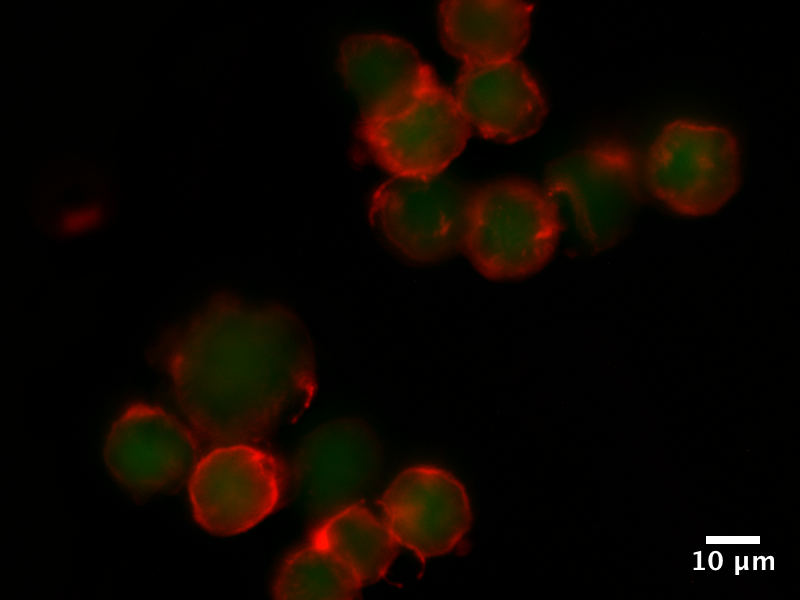
\includegraphics[width=2.3in]{FinalOverlay_Crop.png}
\caption{\textbf{Staining of non-adherent cells}. Images of LNCaP cells seeded into a device and stained immediately after seeding. EpCAM (red), GFP (green).}
\label{fig:staining}
\end{figure}

\subsection{Cell Culture}

We have used the devices presented here to culture multiple cell lines (MC3T3-E1, PC3, MCF7, and LNCaP). Initial results suggest that cell viability is not affected in any way by the process of cell concentration (data not shown). However, as with any cell-based assay, results are dependent upon many factors including the cell type and sample source. Thus, any potential bias of using this method would have to be evaluated on a case-by-case basis.

\section{Conclusions}

We have presented a method to simultaneously concentrate a suspension of cells and seed them into a microchannel that can be used for culture and the gentle application of treatment protocols. We were able leverage dimensional analysis to lower cell loss to 1.1 $\pm$ 0.6\% (avg $\pm$ SD, n = 7) via changes in device dimensions and flow rates. Data that suggests the ratio of the characteristic settling time of a cell to the estimated residence time of the cell in the collection region can be used to predict changes in cell loss with changes in device geometry and pumping parameters. Experimental data obtained under various conditions using two different device designs suggests that efficient device operation in terms of cell loss and throughput is achieved when $t_{set}/t_{res} \approx 1$. When using this method, the maximum possible cell loss is dictated by the volume used for each addition and is an important parameter to consider when attempting to reduce cell loss. Dimensional analysis suggests that the viscosity of the fluid and height of the collection region do not influence cell loss in this type of embodiment whereas the size of the cell, travel distance through the collection region, and flow rate do. The device and method increase the range of cell suspension densities that can be used with cell-based assays performed using microscale devices and provides an alternative when centrifugation is inadequate as a method for sample concentration. In this way, the technology helps to enable research on rare cell populations such as cells isolated using flow cytometry, circulating tumor cells, or primary samples from small animals. 

Specifically, we plan to use the presented microfluidic device to enable functional studies of patient CTCs. By concentrating more CTCs into fewer devices, our goal is to increase the potential for successful culture and assessment of CTCs. The ability to study CTCs on the microscale using more sensitive assays that are well-suited for limited numbers of cells could lead to less invasive monitoring of cancer treatment efficacy and a better understanding of the molecular mechanisms of cancer metastasis.

\section{Acknowledgement}

The authors would like to thank Erwin Berthier and Dr. Scott Berry for their help and suggestions with modeling and dimensional analysis of the device.  This work was supported in part by the Wallace H. Coulter Translational Research Partnership, the Department of Defense Prostate Cancer Research Program (DOD PCRP Idea Award, W81XWH-09-1-0192), and the University of Wisconsin Carbone Cancer Center.

\chapter{Components: `The Oscillator' for Adhesion and Shear-Stress Assays}
\label{Chap:Oscillator}

\section{Preface}
This chapter represents a manuscript in preparation. 

\section{Introduction}
This chapter describes the development of a modular oscillatory flow method. Although oscillatory flow could be used in a variety of ways, this component was developed to enable cell-based adhesion assays. Currently, functional cell adhesion assays are implemented using a few approaches: atomic force microscopy (AFM), micropipette manipulation, centrifugation, and fluid flow (see review \cite{Christ:2010ly}). The first two methods are intended for studying single cells and require significant expertise and are not appropriate for characterizing populations of cells. Centrifugation is simple and integrates well with a laboratory setting yet it cannot be used to interrogate aspects of dynamic cell adhesion (i.e. when the cell is attempting to adhere to a substrate in the presence of fluid flow using relatively weak, non-specific interactions) and cannot mimic physiologic fluid shear-stresses which have been shown to be important in subsequent static adhesion processes (i.e. formation of high-strength anchoring points to the substrate or cell neighbors) \cite{Sengbusch:2005zr}. Current methods that use fluid flow employ the use of spinning discs, microfluidic flow-through chambers, or simply pipetting fluid over cells. Spinning disc assays can typically only be used for studying static adhesion characteristics. Flow-through chambers employ the more physiologic phenomena of fluid shear-stress and are well-suited for microscopes to allow study of both dynamic and static adhesion events but require expensive equipment (syringe pumps, $\ge$ \$1000) to produce the fluid flow and have challenges in terms of usability due to the syringes, tubing, and fluidic connections required. Manual pipette-driven flow is simple but highly variable and the resulting data is only marginally quantitative, yet appears to be an accepted method in some areas of biology. The method presented here shares the advantages of other flow-based methods, such as the ability to study dynamic and static adhesion processes, but eliminates the costly syringe pumps and cumbersome tubes and fluidic connections. The act of connecting and maintaining tubes is replaced by the act of placing a cantilever on a membrane much like a record needle is placed to play music on a record player. The approach also allows samples to be loaded and removed using a common pipette. 

In order to validate the use of this technology in cell-based adhesion assays, the performance characteristics of the system must first be characterized. After the technical characterization, a biological validation can then be performed (see Chapter \ref{Chap:TumorCellAdhesion}). 

\section{Approach}
The device consists of a flexible PDMS diaphragm that is placed over an open microfluidic port to create a small, sealed air chamber. The diaphragm is actuated using a piezoelectric bender-actuator that responds linearly to voltage signals to induce changes in pressure that result in fluid flow.

\begin{figure}[!ht]
\centering
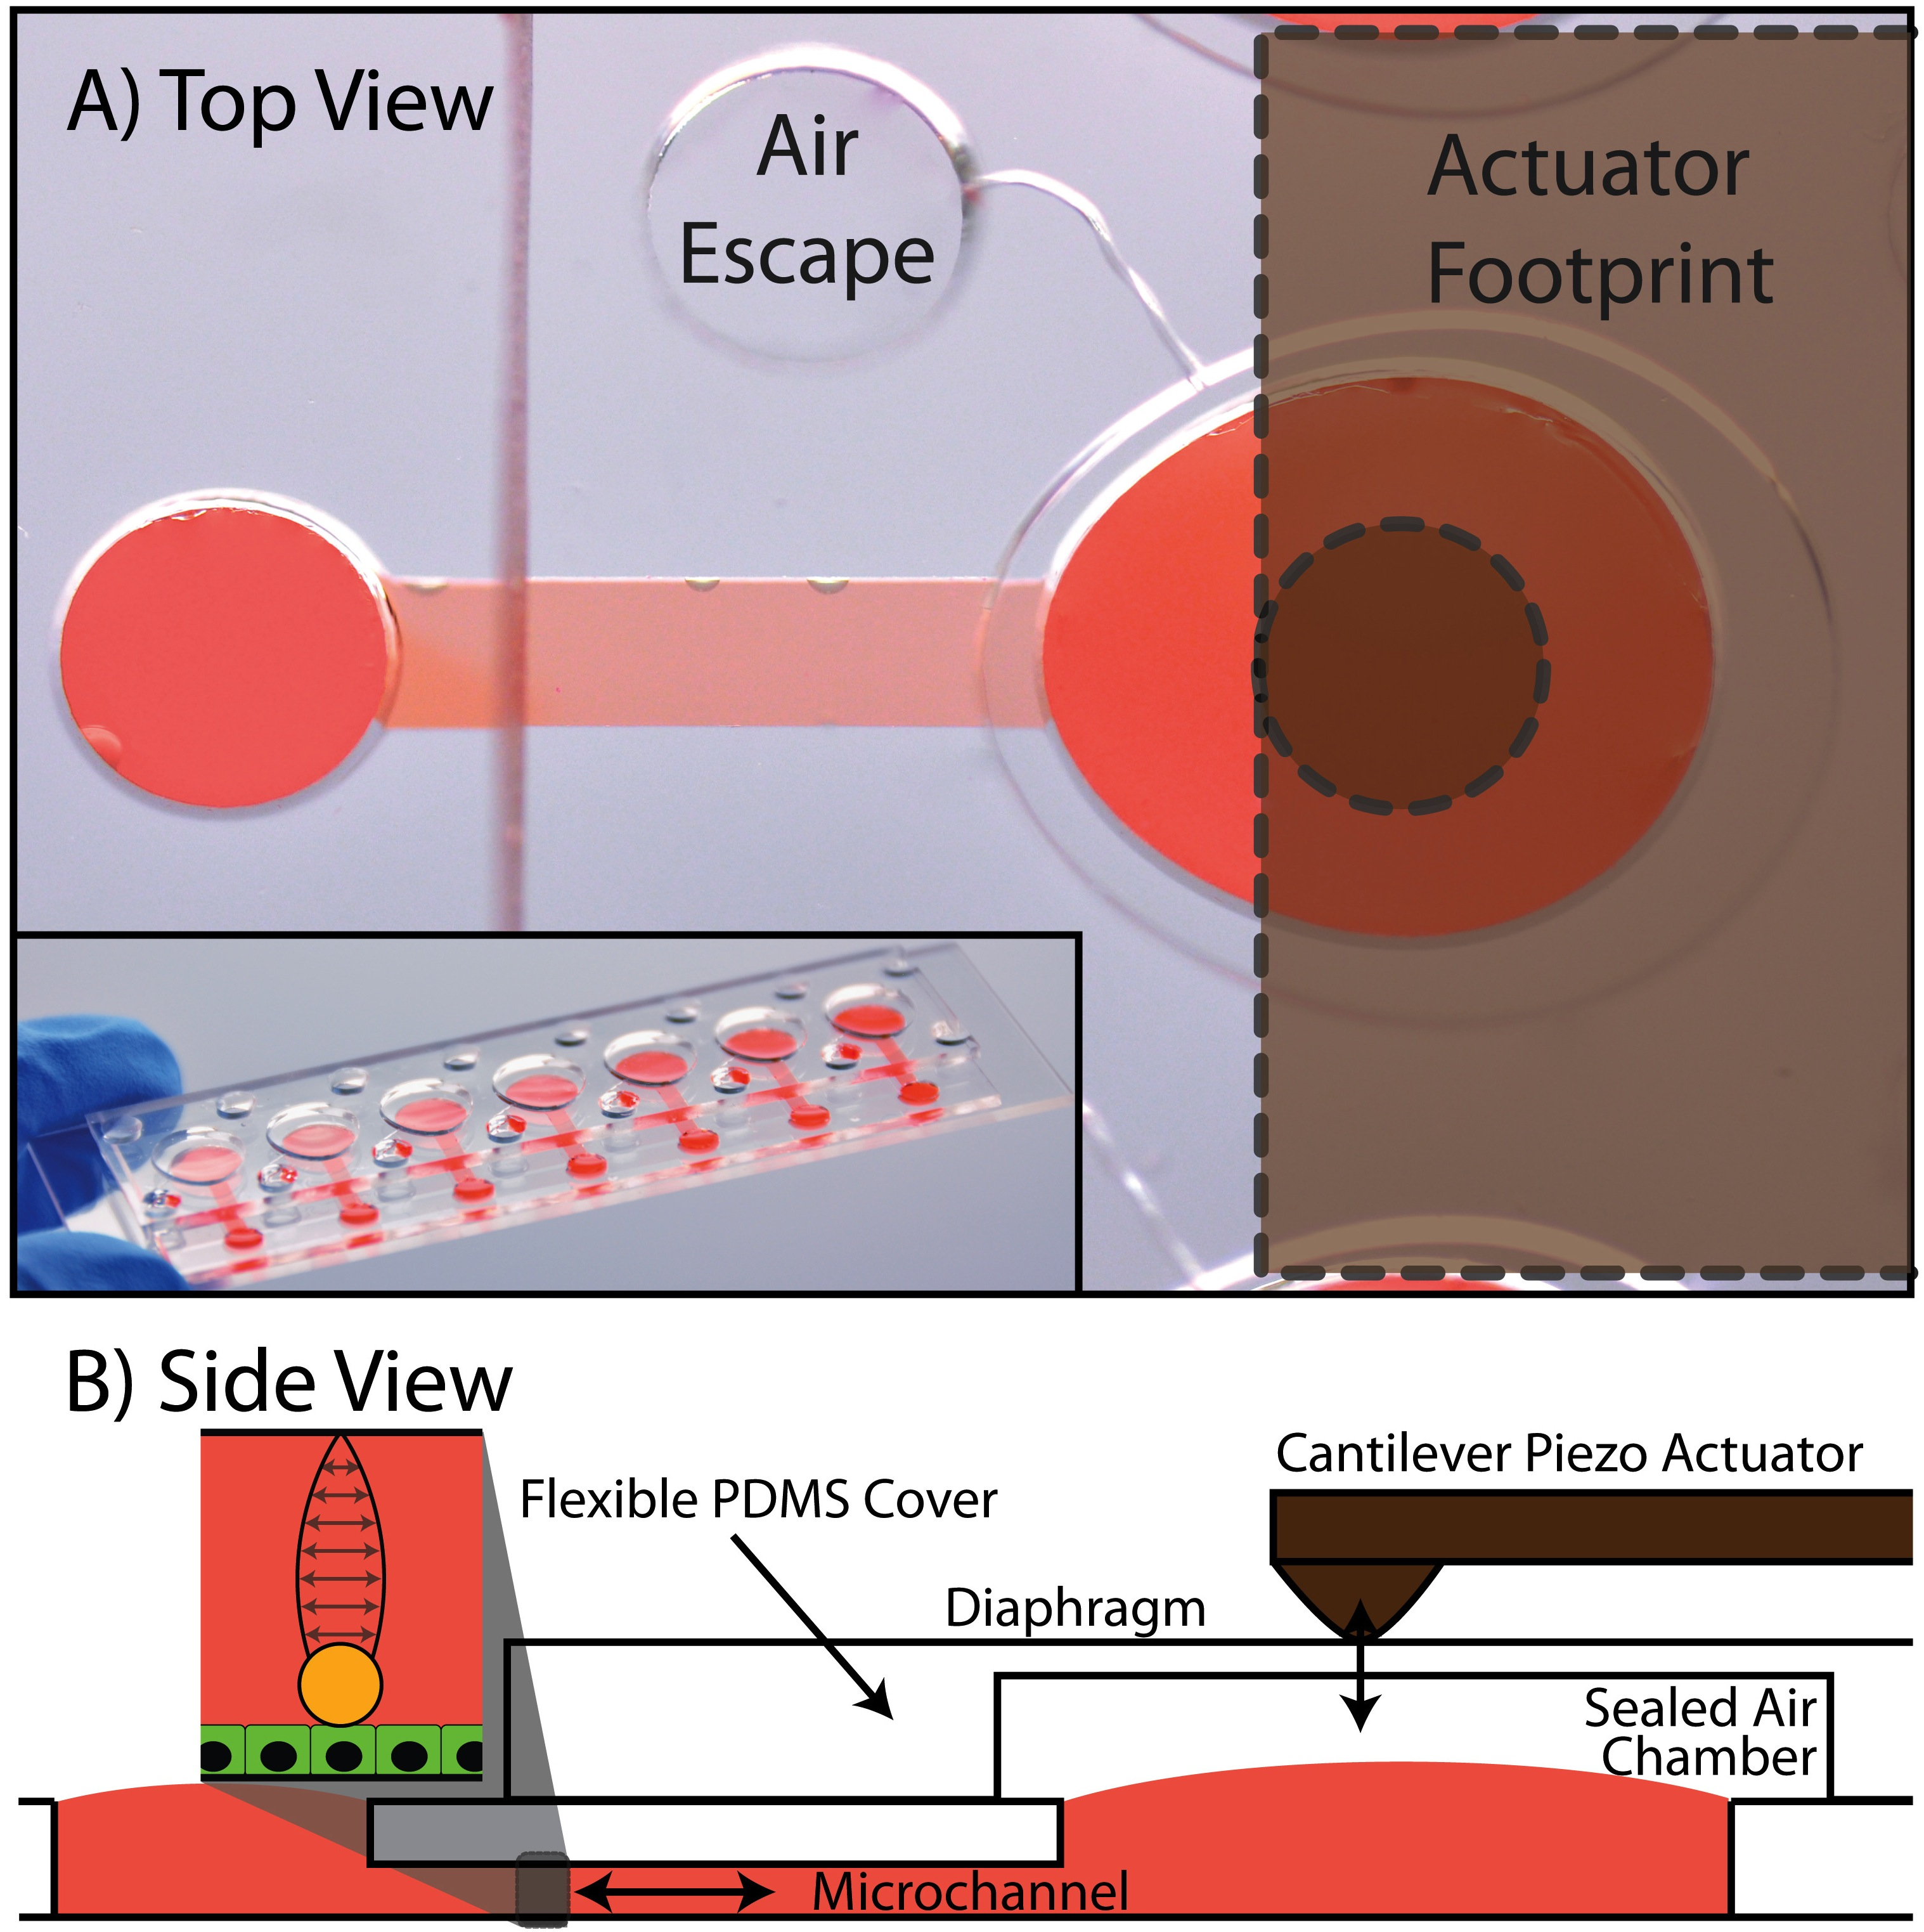
\includegraphics[width=3.5in]{OscillatoryDiagram3.jpg}
\caption{\textbf{Oscillatory flow setup}. Image of diaphragm placed over the port of a microchannel. Inset illustrates ability to array the methodology. The bender-style actuator can be made with multiple fingers or extensions to allow actuation of multiple channels at once. Similarly, the pressure at one port can be multiplexed to multiple channels.}
\label{Chap:Oscillator:Schematic}
\end{figure}

Actuation of the diaphragm was accomplished using a 3.5 cm $\times$ 1.3 cm $\times$ 0.3 cm bender-style piezo actuator (Q220-A4-303YB - Piezo Systems, Inc. Woburn, MA) with a piece of plastic and cap screw fixed to the end in order to make a focused point of contact with the diaphragm. Other non-piezo methods of actuation can be used but a piezo actuator offers the benefit of having no moving parts (\eg\, gears or ball-bearings); instead, the ceramic material bends upon application of a voltage making it more amenable to challenging environments such as incubators. A bender-style piezo actuator (flat and long like a stick of gum) is used because of the `large' range of motion that can be produced compared to other styles. One drawback of bender-actuators is that the force produced is relatively small ($<$ 1N) compared to some other designs ($>$ 1000 N). The actuator responds linearly to voltage. However the voltage levels are significantly higher than the 0-10V outputs of most signal generators. For this reason, signals are first passed through a piezo amplifier (PN: VP7206-24L105 - Viking Industrial Products. Marlboro, MA). Signals are generated using a 33220A waveform generator (Agilent Technologies Santa Clara, CA). Although a signal generator is used here, the amplifier is able to accept `mono' voltage signals coming from a headphone jack of a computer to enable simple software solutions for signal generation. Additional device setup is described in Section \ref{Chap:Oscillator:sec:methods:deviceSetup}.

\section{Characterization and Discussion}
Characterization begins with measurements of actuator response and is followed by analysis of flow within the microchannel. Given the focus here on adhesion assays, wall shear-stress is used as the primary metric of system response.

\subsection{Actuator Response}
Fig \ref{Chap:Oscillator:fig:actuatorResponse} shows how the actuator responds to voltage as well as its frequency-response. These tests were performed using the fully assembled actuator and tip but without being in contact with the diaphragm.  The actuator voltage-response was linear while the frequency response illustrates constant amplitudes below 20 Hz and a resonant frequency that was greater than 80 Hz.

\begin{figure}[!b]
\centering
\begin{tabular}{p{0.3cm}cp{0.3cm}c}
A) & \imagetop{\includegraphics[width = 2.5in]{PizeoVoltageResponse.pdf}} & B) &
\imagetop{\includegraphics[width = 2.5in]{PiezoFrequencyResponse.pdf}}\cr
\end{tabular}
\caption{\textbf{Voltage and frequency response of piezoelectric bender-actuator}. A) Actuator amplitude is linear to the input voltage. B) Actuator amplitude was constant below 16 - 32 Hz. The resonant frequency is $>$ 80 Hz.}
\label{Chap:Oscillator:fig:actuatorResponse}
\end{figure}

It is expected that coupling of the actuator with the microchannel and membrane will alter the frequency response, likely damping the resonance observed at high frequencies.

\subsection{Shear-Stress Response}
Excluding the frequency response of the actuator, there are two characteristic frequencies of this diaphragm-microchannel setup. The first dictates the transition from quasi-steady flow to pulsatile flow while the second marks a transition in the behavior of the pumping mechanism from being much like a syringe pump to being like a regulated pressure source. These transitions are discussed more fully in the next two sections.

\subsubsection{Flow Transition: Quasi-steady \vs\ Pulsatile}
The Womersley number can be used to help characterize the pulsatile nature of the flow (Eq \ref{Chap:Oscillator:equ:womersley}) as it provides a measure of the balance between viscosity and momentum effects induced by oscillatory motion. 

\begin{equation}
\Omega = a \sqrt{\frac{2 \pi f \rho}{\mu}}
\label{Chap:Oscillator:equ:womersley}
\end{equation}
 
In Appendix \ref{App:Oscillator}, it is shown that the critical value for the Womersley number in PPFCs is 2.8 where the height of the PPFC is used as the critical length dimension, $a$. The dimensions of the simple one-input-one-output channel used in these studies are L $\times$ W $\times$ H = 7.5mm $\times$ 1.5 mm $\times$ 0.228 mm. Given these channel dimensions, previous work by Bacabac \etal\ suggests that the shear-stress will remain linear with pressure-gradient below 4.8 Hz. This can be seen in Fig \ref{Chap:Oscillator:fig:flowTransition} where pulsatile-flow shear-stress is normalized by steady-flow shear-stress calculated using the same pressure gradient. At low frequencies, the two models predict the same shear-stress whereas the pulsatile model attenuates above the transition frequency. Shear-stress attenuates due to inertial effects induced by high frequency oscillations.

\begin{figure}[!ht]
\centering
\includegraphics[width=3.5in]{Pulsatile_vs_SteadyShear2.pdf}
\caption{\textbf{Transition from steady to pulsatile flow}. The influence of non-parabolic flow profiles can be seen on shear-stress for frequencies above the transition frequency of 4.8 Hz. This simulation keeps pressure constant while varying frequency. Shear stress is normalized to the shear stress measured at the lowest frequency, which is nearly identical to the steady-flow solution for the same pressure gradient.}
\label{Chap:Oscillator:fig:flowTransition}
\end{figure}

\subsubsection{Pumping Transition}
The ports and air chamber of the oscillatory flow setup act as capacitors with the microchannel acting as a resistance between them. At low frequencies, the capacitors are negligible and the volume displaced in the channel is equal to the volume of air displaced by the actuator\slash diaphragm. At high frequencies, the resistance of the channel impedes charging and discharging of the capacitors, leading to a situation where fluid displacement is less than the air displaced by the actuator\slash diaphragm. This can be seen in a plot of simulation results (for methods see Section \ref{Chap:Oscillator:sec:methods:shear}) where the ratio of the air displaced by the diaphragm is compared to the fluid displacement in the channel for a range of frequencies (Fig \ref{Chap:Oscillator:fig:pumpingTransition}). At low frequencies, the pumping mechanism behaves much like a syringe pump and falls rapidly when above a certain cutoff frequency. This transition in the pumping behavior can be roughly estimated by calculating the capacitance of the air chamber ($C = $3.8e-13 [m$^{3}$/Pa]) and the resistance of the microchannel ($R = $3.95e9 [Pa-s/m$^{3}$]). The characteristic frequency of the transition can then be calculated using an RC-circuit analogy where $f = 1/(2\pi RC) = 106$ Hz, which represents the frequency at which signal should be attenuated by roughly half. This calculation agrees very well with the simulation results. Although the transition is predicted to be near 106 Hz, the initial effects of the transition can be seen earlier, at $\sim$ 30 Hz. Still, the pumping transition frequency is well above the flow transition frequency; thus, the range where shear-stress increases linearly with frequency is limited by the physics of pulsatile flow within the microchannel rather than the pumping mechanism. The pumping transition frequency can be increased if necessary by reducing the volume in the air-chamber to create a stiffer capacitor (\ie\, lower capacitance).

At extremely high frequencies, the fluid displacement will be negligible compared to the air-volume displaced by the actuator\slash diaphragm, resulting in what behaves like a pressure-based pump rather than a volume-based pump like a syringe-pump where all lines are completely filled with fluid.

\begin{figure}[!ht]
\centering
\includegraphics[width=3.5in]{ChannelFrequencyResponseTheory2.pdf}
\caption{\textbf{Transition from syringe-pump-like behavior to pressure-driven behavior}. Normalized volume displacement represents the ratio of the air-volume displaced by the actuator to the volume of fluid displaced in the channel. Simulation suggests that at low frequencies, the air and fluid displacement are tightly coupled with a ratio of almost 1. At higher frequencies, the capacitance of the air chamber coupled with the resistance of the microchannel result in a coupling that is less than 1, approaching 0 when $f \gg 106 Hz$.The capacitance of the air chamber and resistance of the channel suggest a pumping transition frequency of roughly 100 Hz which coincides with simulation results.}
\label{Chap:Oscillator:fig:pumpingTransition}
\end{figure}


\subsubsection{Overall System Response}
Overall System response was measured experimentally to observe change in shear-stress with respect to both frequency and actuator amptlitude\slash voltage

\begin{figure}[!ht]
\centering
\includegraphics[width=3.5in]{ChannelFrequencyResponse.pdf}
\caption{\textbf{Channel frequency response}. }
\label{Chap:Oscillator:fig:channelFrequencyResponse}
\end{figure}

Fig \ref{Chap:Oscillator:fig:channelFrequencyResponse} shows the frequency response at an actuator voltage of 100 mV. Experimental measurements of shear-stress were obtained from observations of particle motion as described in Section \ref{Chap:Oscillator:sec:methods:shear}. As predicted in the previous discussions of the flow and pumping transition frequencies, shear-stress is linearly related to frequency below 5 Hz. Above 5 Hz, the influence of non-parabolic flow profiles and air-chamber capacitance can be seen to influence the linear relationship.

In Fig \ref{Chap:Oscillator:fig:channelVoltageResponse}, shear-stress was measured in the channel across a range of voltages for three different frequencies (for methods see Section \ref{Chap:Oscillator:sec:methods:shear}). Shear-stress changed linearly with voltage at each frequency. Measurement variability increases with frequency and voltage given the measurement method used here. Acoustic streaming increases with frequency and induces particle motion that makes it more difficult to determine amplitude in the center streamline. Similarly, at high voltages, it can be difficult to observe a full oscillation of particle motion in one field of view of the microscope camera. The linear behavior is expected given the linear relationship between pressure-gradient and shear-stress in the equations outlined in Appendix \ref{App:Oscillator} for pulsatile flow.

\begin{figure}[!ht]
\centering
\includegraphics[width=3.5in]{ChannelVoltageResponse.pdf}
\caption{\textbf{Channel voltage response}. Shear-stress is measured across a range of piezo voltages for three different frequencies. Each series of points indicates linear relation ship between shear-stress and voltage, which is in agreement with simulation as well (see App \ref{App:Oscillator}).}
\label{Chap:Oscillator:fig:channelVoltageResponse}
\end{figure}

\section{Methods}
\subsection{Actuator Motion Measurements}
Motion was measured using bright-field microscopy where the actuator was mounted on its side such that the tip appeared to move side-to-side in the field of view. Motion was quantified from digital images.

\subsection{Fluid Flow Modeling and Shear-Stress Estimation}\label{Chap:Oscillator:sec:methods:shear}
The microfluidic channel was approximated as a parallel-plate flow-chamber (PPFC). Fluid flow was modeled using methods for both steady-flow and pulsatile-flow where flow is laminar. Modeling of the flow transition frequency utilized the pulsatile flow model whereas modeling of the pumping transition frequency used the steady flow model. The steady flow model is needed in this case in order to separate effects of flow transition from pumping transition. These equations for steady and pulsatile flow are given in Appendix \ref{App:Oscillator}. 

Fig \ref{Chap:Oscillator:fig:amplitudeMeasurements} compares the use of a steady and pulsatile model of flow for determining shear-stress from particle amplitude. In this graph, the magnitude of the pressure gradient is held constant while frequency is changed. For each frequency, the pulsatile model is used to determine the amplitude of the fluid motion in the center streamline. This amplitude is then used in the steady-flow equation for determining shear-stress from particle amplitude (Appendix \ref{App:Oscillator}). The results show that the amplitude of the fluid motion can be used to predict shear-stress using an assumption of a parabolic flow profile with $<$ 5\% below 32 Hz and $<$ 1\% below 13.8 Hz. This helps to make estimation of shear-stress from measured particle-amplitudes a much easier calculation for experimentation. However, given the pulsatile model is in place, the pulsatile model was used for all experimental measurements.

\begin{figure}[!ht]
\centering
\includegraphics[width=3.5in]{Pulsatile_vs_SteadyShear.pdf}
\caption{\textbf{Shear-stress from particle amplitude}. (solid-black) Shear-stress is plotted \vs\ frequency using the pulsatile model of flow in a PPFC. (dotted) The dotted line indicates the shear-stress that would be predicted if one were to measure particle amplitude in the channel and use a parabolic flow profile assumption to predict the shear-stress. (solid-gray) The solid-gray line indicates the error relative to the non parabolic line. Error is plotted at the same scale as normalized shear-stress with potential values between 0 and 1. The error line suggests error is $<$ 5\% below 32 Hz and $<$ 1\% below 13.8 Hz.}
\label{Chap:Oscillator:fig:amplitudeMeasurements}
\end{figure}

Shear-stress was estimated using particle motion. Particle motion was measured using 15 \textmu m fluorescent beads (PN:F8843 - Invitrogen. Eugene, OR) on an inverted fluorescent microscope (PN:IX70 - Olympus. Center Valley, PA) equipped with a digital camera (PN:C4742-80-12AG - Hamamatsu, Hamamatsu City, Japan) and MetaMorph imaging software (Molecular Devices. Sunnyvale, CA). While oscillating the particles, the channel was flipped upside-down to cause the beads to settle to the ceiling of the microchannel. This was done while actuating the channel. After 1.5 min, the channel was placed rightside-up on the microscope. The exposure time for each image was set to capture at least one full cycle of bead motion in a single image, making the bead appear as a streak. The images were captured in rapid succession using the `Acquisition Stream' function of MetaMorph to record particle amplitude as it settled from the ceiling to the substrate. Roughly 30 images are acquired during settling providing ample opportunity to select a frame in which a bead near the center portion of the channel reaches its maximum amplitude. The pixel length of the streak is recorded and converted to an amplitude in meters which is then converted to a shear-stress in Pa using a pulsatile model of flow to relate amplitude with shear-stress.

This method of shear-stress determination becomes more challenging at high frequencies and amplitudes. At high amplitudes, the entire particle motion can extend beyond the view-field of the camera. At high frequencies acoustic streaming can occur near device edges and bubbles to disturb cell settling and make it difficult to ensure the particle is traveling through a position where it will exhibit its maximum displacement \cite{Chung:2008fk}. Also, at high enough frequencies, the maximum fluid-displacement does not occur at the center streamline. Although not quantified here, it is estimated that this effect could be noticed in the image sequences at frequencies above 20 Hz. Although challenges in shear-stress determination can occur at high amplitudes and frequencies, overall, the method is repeatable (see Fig \ref{Chap:Oscillator:fig:channelFrequencyResponse}), fast, and appropriate for channel calibration in adhesion assays where physiological frequencies are $\sim$ 1 Hz and attachment occurs at shear-stresses $<$ 1 Pa. In roughly 2 minutes, the shear-stress in the channel can be determined and repeated to within a couple pixels.

\subsection{Device Setup}\label{Chap:Oscillator:sec:methods:deviceSetup}
The microchannel and diaphragm design are illustrated in Fig \ref{Chap:Oscillator:fig:deviceDesign}. The components were made from polydimethylsiloxane (PDMS).

\begin{figure}[!ht]
\centering
\includegraphics[width=1.5in]{MicrochannelDesign.pdf}\hspace{0.5cm}\includegraphics[width=1.5in]{DiaphragmDesign.pdf}
\caption{\textbf{Device design}. Microchannel: 0.228 mm $\times$ 1.5 mm $\times$ 7.5 mm (from inside edge of input to inside edge of output). Channel input port: 1.5 mm radius. Channel output port: 6.24 mm $\times$ 5.6 mm. Air chamber: 7 mm $\times$ 7.8 mm $\times$ 1 mm. Air escape channel: 50 \textmu m tall $\times$ 100 \textmu m wide. Air escape port: 3 mm radius. The diaphragm is the ceiling of the air chamber. The thickness of the diaphragm is determined by the difference in thickness between the air chamber feature an air escape port, which is estimated to be 250 \textmu m.}
\label{Chap:Oscillator:fig:deviceDesign}
\end{figure}


The PDMS microchannel devices were first placed in OmniTrays (Thermo Fisher Scientific. Rochester, NY) and filled with PBS containing 0.5\% BSA to discourage beads from sticking to each other or the walls of the device. The diaphragm is placed over the large port of the device while leaving the small port exposed to the atmosphere. The air escape allows fluid to be loaded while the diaphragm is already in place. Without the air escape, fluid cannot be loaded efficiently due to the relative capacitance of the exposed port and sealed air chamber.

Within the OmniTray, a metal strip is fixed to the bottom using double-sided tape. The actuator, mounted to a 1 cm $\times$ 2.5 cm piece of plastic via double-sided tape is held in place on the metal strip with magnets fixed to the actuator assembly. This provided an easy means to place and remove the actuator. The position of the actuator was able to remain very stable during manipulation of the OmniTray, enabling the flip technique for shear estimation. The cap screw used as the point of contact between the actuator and diaphragm provided height adjustability where needed. The entire assembly could be enclosed in a covered OmniTray. The lid provided enough compliance for the small wires leading to the piezo-actuator.

The actuator is placed on the diaphragm just prior to experimentation but can be put in place earlier if desired. The voltage and frequency of oscillation are set and the beads are loaded. After loading, the air escape is plugged using a drop of bead suspension or other fluid that will pin at the entrance to the air escape port.

Immediately after loading, the microscope is focused on the beads and the entire OmniTray is flipped and placed on a surface to remain level for 1.5 min to allow the beads to settle to the ceiling for subsequent imaging. After each set of images, the OmniTray is flipped again to reset the beads to the ceiling and allow for a repeat of the measurement. 

\section{Other Potential Applications}
Although the device is aimed at use for performing cell-based adhesion and shear-stress assays, the oscillatory pressure source could be used of other things as well. For example, the oscillating pressure can be rectified to produce net flow in one direction or recirculatory flow\cite{Leslie:2009vn,Seker:2009uq}. It has also been shown that the oscillatory nature of pumps can be used with high and low pass filters to produce tunable `valving' for other behavior within a device\cite{Mosadegh:2010kx}. Also, the oscillating air pressure can be used as well to drive fluid in other ways\cite{Langelier:2009qm}. Given the lack of moving or rusting parts, the method is also amenable to prolonged exposure within incubators for long-term application of shear-stress.

\section{Conclusions}
A tubeless method for producing oscillatory flow in microchannels has been presented. The method addresses various shortcoming of other methods to provide a tubeless method method for producing quantifiable oscillatory shear-stress in a microchannel that can be addressed using a pipette or liquid handling automation. The device analyzed here shows a linear shear-stress response to changes in frequency below 5 Hz but is capable of providing complex signals with much higher harmonics (up to $\sim$ 30 Hz) with the understanding that non-parabolic flow profiles and inertial considerations begin to add non-linearity to the response. Two characteristic frequencies determine the behavior of the device, the flow transition frequency, dictated by the Womersley number, and the pumping transition frequency, dictated by the resistance of the microchannel and dimensions of the air chamber. Transition between quasi-steady and pulsatile flow occurred near 5 Hz while the pumping transition frequency was estimated to be near 100 Hz suggesting syringe-pump-like behavior below 30 Hz.







\chapter{Assays: Cell Adhesion Assay Validation: Tumor-Cell Adhesion to a HUVEC Monolayer}
\label{Chap:TumorCellAdhesion}

\section{Preface}
This work was performed and written in equal collaboration with Edmond Young as represents a manuscript in preparation.

\section{Introduction}
The process of cell adhesion involves physical interactions between cells and the materials in their microenvironment such as extracellular matrices, synthetic biomaterial surfaces, and other cells and is a major topic of interest in areas ranging from fundamental cell biology and pathophysiology \cite{Chen:1997p320,Davies:1995p87} to tissue engineering and regeneration \cite{Nugent:2003p459}. In particular, cell adhesion plays an integral role in inflammation and cancer metastasis where leukocytes and circulating neoplastic cells, respectively, interact with the vascular endothelium in complex adhesion cascades that include tethering, rolling, spreading and endothelial transmigration events \cite{Ley:2007fk,Geiger:2009vn}. The ability to examine and measure the propensity of cells to adhere to the endothelium or other surfaces (engineered or natural) and determine the strength of adhesion is thus critically important to advancing our understanding of the mechanisms related to inflammation and cancer and to the development of tissue engineering strategies in regenerative medicine.

While cell adhesion fundamentally relies on the biophysical and biochemical properties of individual cells \cite{Orsello:2001uq}, many adhesion studies use population-based assays to determine global adhesion characteristics that efficiently reveal important and relevant properties of the cell population \cite{Christ:2010ly}. Population-based adhesion assays typically depend on fluid-flow systems that generate mechanical shear-stress, providing means to promote or challenge adhesion to the substrate on interest in a controlled manner. The most common fluid-flow systems for studying cell adhesion include the parallel-plate flow chamber \cite{GIAVAZZI:1993ty}, radial flow chamber \cite{Goldstein:2002p106}, cone-and-plate viscometer \cite{Jadhav:2001ys}, variable width devices \cite{Heilshorn:2003ly,Usami:1993p603}, and variable-height chambers \cite{Xiao:1996p618}. These systems typically employ steady flow conditions, but they can also be readily modified to accommodate oscillatory or pulsatile flow conditions for studies in shear-mediated atherosclerosis and cardiovascular pathobiology \cite{KU:1985uq,Chappell:1998fk}. Depending on the purpose of the study and availability of resources, flow systems can be operated under various schemes or protocols to produce different types of adhesion assays. For example, flow-rate\slash shear-stress can either be increased or decreased in a stepwise fashion to assay the gradual detachment or attachment of cells, respectively. Furthermore, shear-stress ranges can be expanded, or the number of steps in the ramping scheme can be increased to yield a more continuous scheme with better resolution for detecting adhesion events than more discrete protocols. Although fluid-flow systems have become indispensable tools in biological research, these systems have significant drawbacks due to their large scale, complex setup, and need for large volumes of medium and cell suspension to maintain flow. 

Recently, a number of microfluidic systems have been developed for cell adhesion and shear-flow assays \cite{Lu:2004ys,Gutierrez:2007p290,Plouffe:2007p274,Young:2007ml}, taking advantage of microfabrication techniques to create systems that can increase throughput, handle reduced fluid volumes, and improve spatiotemporal control of \invitro\ microenvironments \cite{Young:2010p286,Young:2010uq}. While these microscale flow systems have shown improvements over their macroscale counterparts and have overcome some of the main drawbacks of previous systems, the majority of microfluidic systems continue to require complex ``world-to-chip'' interfacing \cite{Fredrickson:2004ve} that limits their potential for widespread adoption in biology labs, particularly in clinical and translational research applications where limited patient-derived cell and tissue samples may be significantly depleted by excessive tubing and large dead volumes. 

We have developed a novel microscale system for conducting oscillatory, shear adhesion assays that employs passive-pumping principles to eliminate cumbersome interconnects and unnecessary tubes and dead volume. The system, described in detail below, enables pipette-based loading and treatments, is easily amenable to complex microscale geometries, and can be dynamically controlled to offer various oscillatory waveforms for cardiovascular applications. Most importantly, this microscale system offers analysis of the adherence of a small and defined population of cells in a manner that cannot be achieved with existing systems, thus enabling studies of limited cell samples such as those acquired from a clinical setting. These capabilities, coupled with a custom information-rich readout, allow this system to be applied to a wide range of biological experiments. To illustrate the potential of this system and custom readout, we developed an attachment-based adhesion assay that utilizes a decreasing log-sweep of shear-stress and differential image analysis of image-streams to quantify the process of adhesion for an entire population of interest. We used the integrated system to study adhesion of three different cancer cell-lines on activated and non-activated endothelial monolayers. Results demonstrate the ability of this approach to provide new insights into the heterogeneity of cell populations and adhesion mechanisms.

\section{Results and Discussion}

\subsection{System Design and Operation}

Our main objective was to design, test, and implement a passive-pumping-based oscillatory flow system for an array of microchannels in order to extend oscillatory modes of shear flow to pipette friendly systems.  Passive-pumping has been used previously in various applications, and has been described in detail elsewhere \cite{Berthier:2007mi,Meyvantsson:2008,Walker:2004ov}. Briefly, passive-pumping leverages surface tension to pump fluid from small droplets to larger droplets based on Laplace's law (Figure \ref{figure:schematic}A). We fabricated a simple one-input-one-output straight microchannel where one port is smaller than the other to facilitate passive-pumping of cell suspensions, media, and reagents. To generate oscillatory flow, we further designed and fabricated a diaphragm from polydimethylsiloxane (PDMS) that was positioned over the larger outlet port and reversibly sealed to the top of the PDMS microchannel. The diaphragm was actuated using a piezoelectric cantilever which bends in response to a voltage signal. The actuator was retrofitted with an adjustable cap screw to provide a single point of contact between the actuator and diaphragm (Figure \ref{figure:schematic}B). Voltage signals were produced using a function generator and passed through an amplifier to the actuator to tunably control displacement of the cap screw tip. The resulting deflections of the diaphragm induce pressure changes within the sealed air chamber below the diaphragm to drive oscillatory flow within the microchannel. The ports act as reservoirs for volume fluctuations with the exposed port providing pipette access to deliver treatments or cell suspension.

\begin{figure}[ht] %DONE
\centering
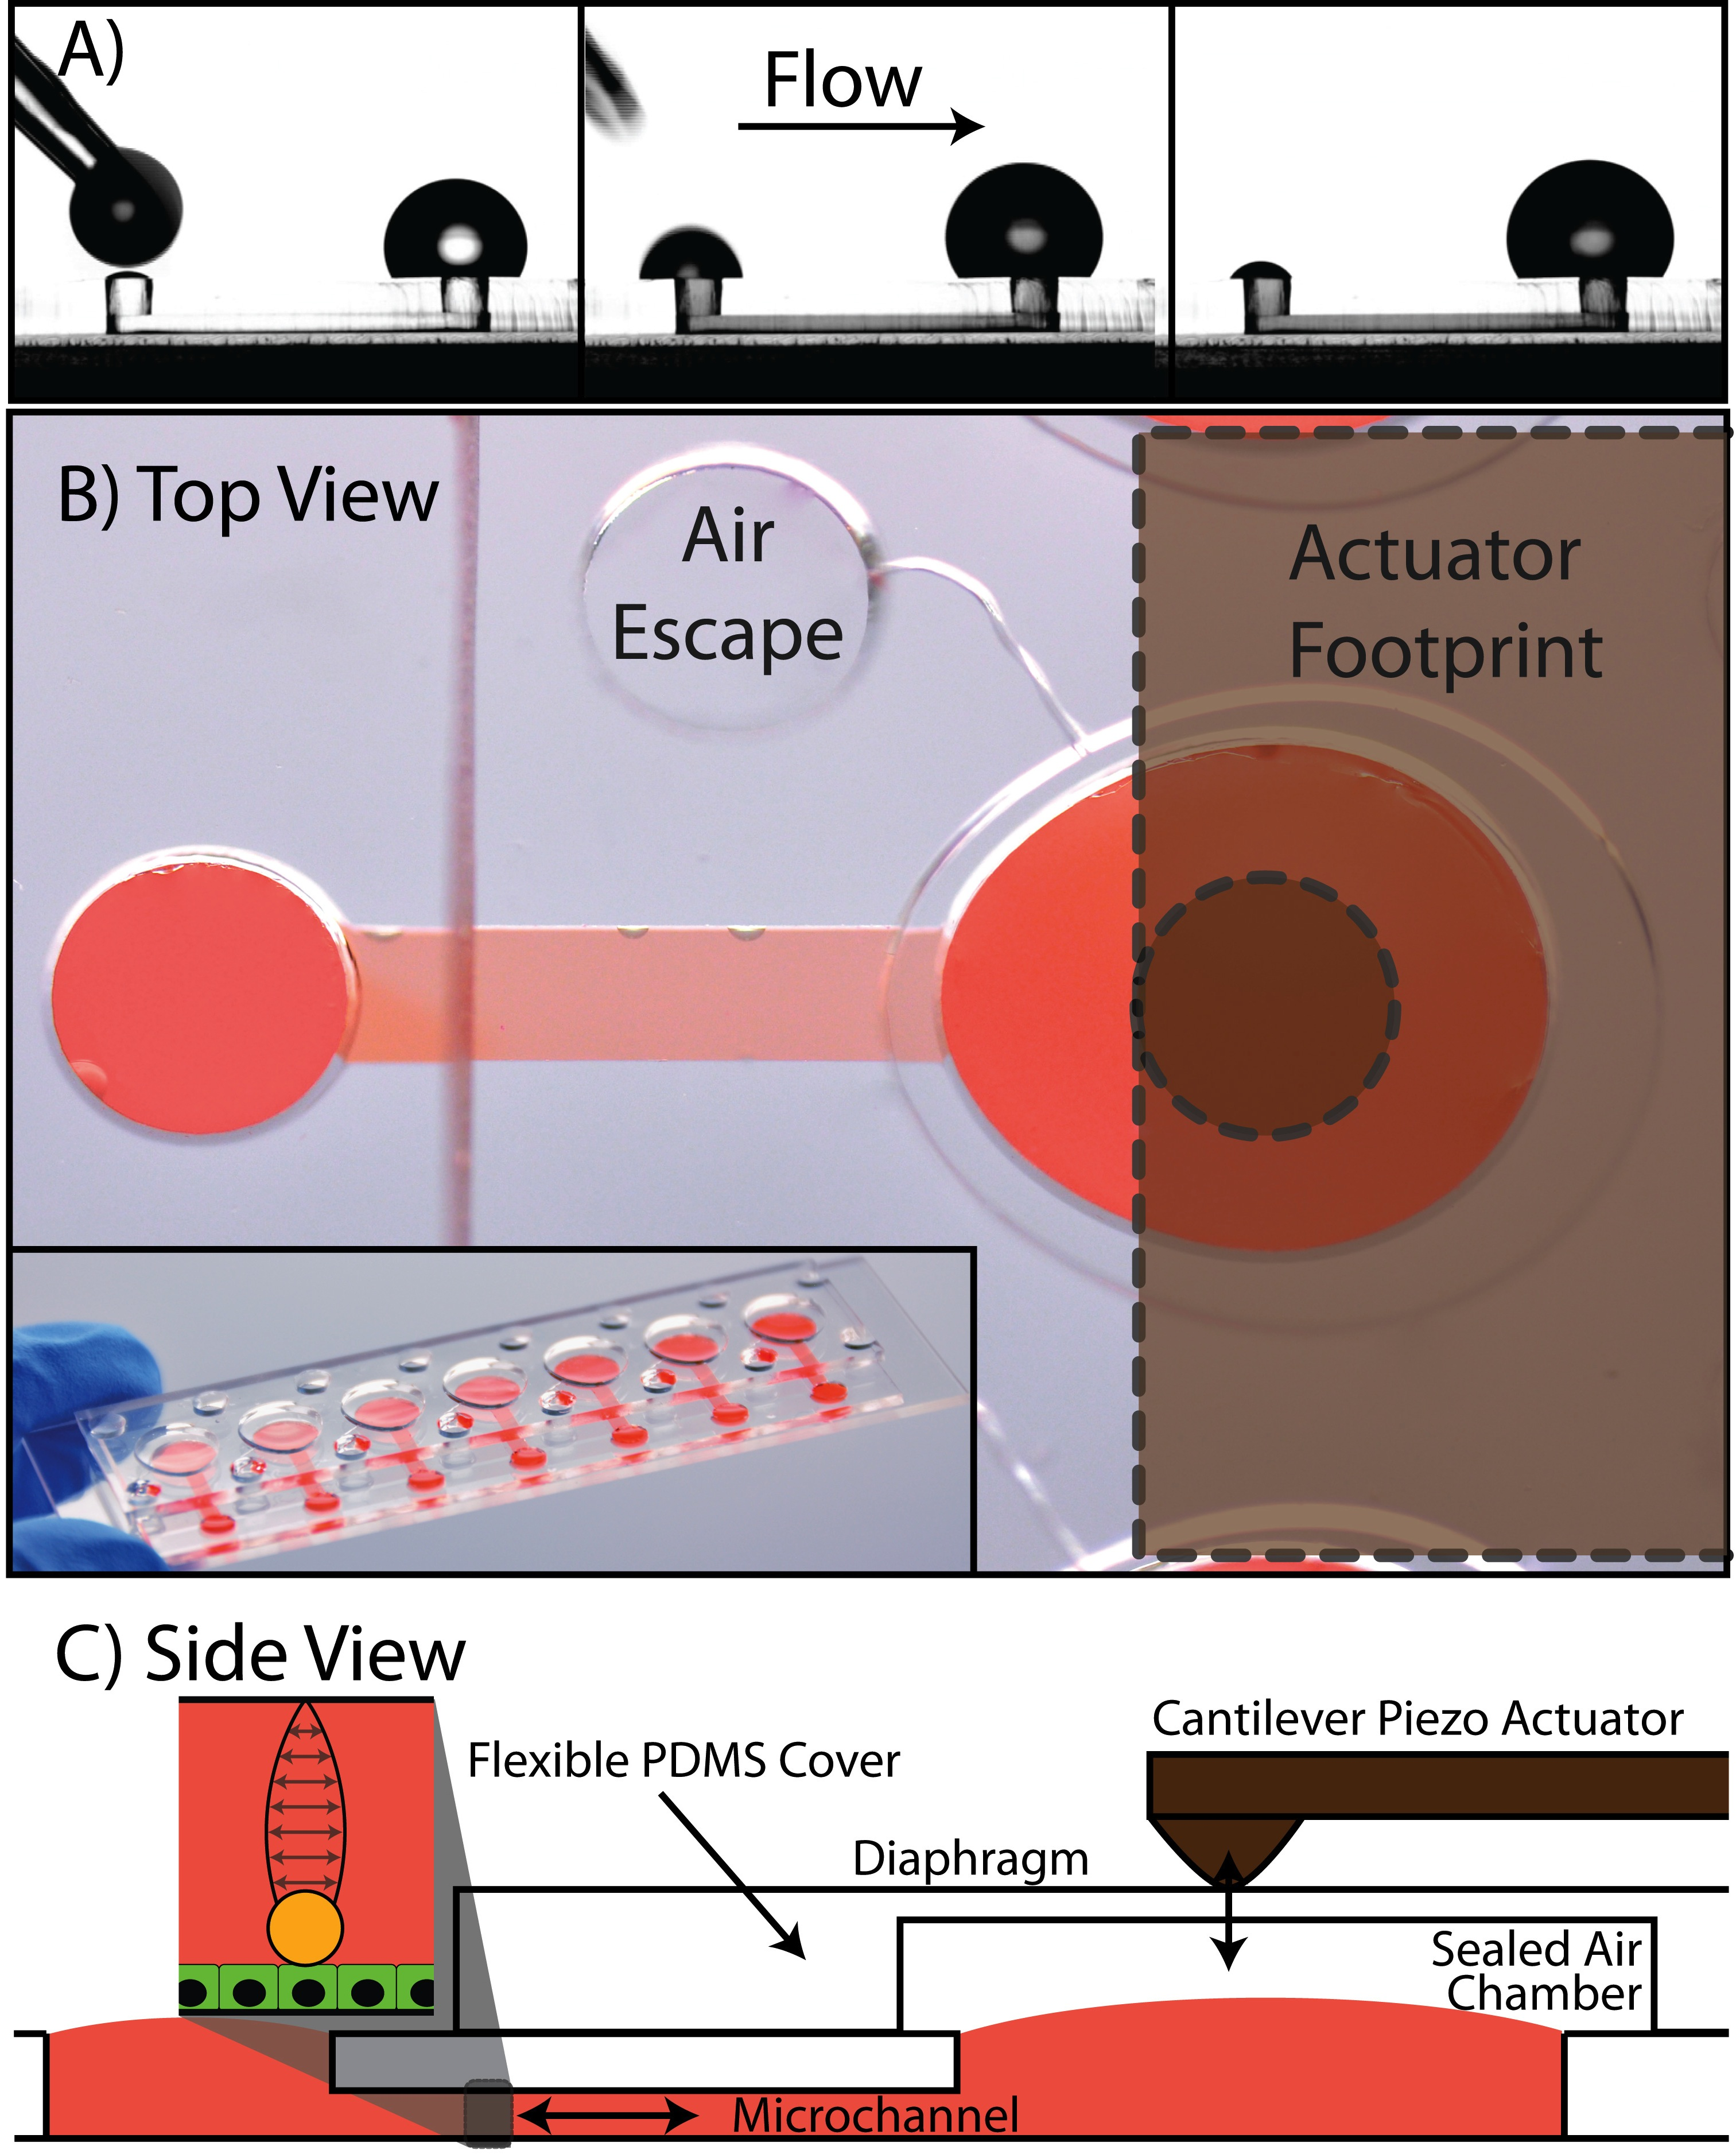
\includegraphics[width=3.5in]{OscillatoryDiagram4.jpg}
\caption{\textbf{Oscillatory flow device}. (A) Side images of passive pumping via dispensed droplets. (B) Top view of microchannel and diaphragm assembly. Inset shows 7 x 1 array of microchannels on a single microscope slide. (C) Side view of setup. Cantilever piezoelectric actuator deflects diaphragm according to applied voltage signals. At low frequency and moderate amplitude, this creates a volume change in the air cavity and displaces fluid in the channel. Oscillatory shear-stresses may be generated with this approach, allowing it to be used for various cell adhesion studies.}
\label{figure:schematic}
\end{figure}

The dimensions of the straight microchannel mimic the dimensions of a conventional parallel-plate flow chamber while the microchannel ports provide the ability to load and treat cells via pipette. The use of microfabrication techniques will allow us to rapidly explore more complex designs in the future. The footprint of the device provides a modest increase in throughput, i.e., up to seven microchannels per array during one microscope acquisition session, but perhaps more importantly, the microchannels were independently addressable. Maintaining separation ensures that each endothelial monolayer is cultured, activated, and\slash or mechanically stimulated as independent biological samples without adverse cross-talk, as is the case in many multiplexed microfluidic systems. In co-culture adhesion studies, this property has the potential for an even larger impact: the system can test limited cell samples, such as those acquired from clinical patients, as demonstrated by our use of $\sim 10^4$ cells per channel. This is a relatively small amount of cells compared to $\sim 10^6$ to $10^7$ cells typically needed for large-scale (mL) continuous flow in parallel-plate flow chambers. We envision that the system can be scaled if necessary to take even fewer cells ($10^2$ or $10^3$ cells), with only minor modifications to microchannel dimensions.

The oscillatory flow methods used here also have potential utility in other biological applications such as cardiovascular and bone mechanobiology, where oscillatory shear-stress has been implicated in important regulatory functions. Macroscale oscillatory flow systems have already been accepted into the laboratory setting while microscale oscillatory systems (and recirculatory systems in general) have also begun to appear \cite{Song:2005p157,Shao:2009p534}; however, the current design is the first oscillatory system to employ passive-pumping, thus combining the advantages of microscale approaches with simple pipette-based operation that obviate the need for tubing that inherently leads to excess dead volume.

The most innovative features of the demonstrated method are the integrated use of the piezoelectric actuator-PDMS membrane, and the development of a unique cell adhesion readout that has potential to offer new biological insights into cell adhesion phenomena. We leveraged the elastic properties of PDMS to create a sealed air chamber and diaphragm with negligible damping effects below 30 Hz and moderate amplitudes. However, oscillatory flow in a microchannel of these dimensions produces non-linear shear-stress response above 5 Hz. Above 5 Hz, the flow profile becomes non-parabolic. Above 30 Hz, the compliance of the air chamber results in significant attenuation of shear-stress. However, a property of laminar flow (steady and pulsatile) is that shear-stress at a given frequency is always linear to the pressure gradient. Clearance between the diaphragm and fluid in the port also limits actuator amplitudes. However, only 30 \textmu m of motion is required to produce the maximum shear-stress used in this study. As mentioned earlier, the microchannel ports act as reservoirs for oscillatory fluid exchange and thus limit the total volume that can be exchanged between the ports per cycle. The adhesion studies to date have been done in the low frequency regime where damping is insignificant leading to a linear relationship between frequency and shear-stress.

\subsection{Adhesion Assay via Image Differencing}

\paragraph{Measurement of Attachment \vs\ Detachment.}The use of a piezoelectric actuator enables the use of a wide variety of signal waveforms and flexible control of the shear-stress protocol. This capability allowed us to develop an 8-minute adhesion assay that samples a large range of frequencies at high resolution using a logarithmic sweep that spans two orders of magnitude (2 Hz to 100 mHz). Thus, this system provides similar resolution to that presented recently by \cite{Christophis:2010fk}. However, in contrast to Christophis \etal\ and other assays that ramp up shear-stress to detect detachment events, we have employed an inverse strategy where cells are initially prevented from adhering by starting at a relatively high shear-stress and then gradually \emph{reducing} shear-stress in order to monitor the \emph{attachment} events instead of \emph{detachment}.

\paragraph{Oscillatory \vs\ Flow-Through Methodologies}Although both oscillatory and flow-through devices can be used to study both attachment and detachment, the use of oscillatory flow fundamentally changes the readout of an attachment assay compared to flow-through devices and provides new insights into adhesion properties that have not been previously obtained. The \emph{attachment} readout of the oscillatory adhesion assay is identical to the \emph{detachment} readout reported by Christophis \etal. In the case of Christophis \etal\, the population of interest is completely defined prior to detachment, enabling them to present detachment results over a range of shear-stresses in terms of ``\% of the entire population of interest''. In doing so, they are able to directly measure the shape of the population distribution with respect to detachment shear-stress. The ability to measure the shape of the population distribution can provide important insight into the mechanisms of adhesion. In our case, the population of interest can also be defined as those cells that are initially in the field-of-view. The oscillatory nature of the flow allows us to monitor this population of interest over time for different levels of shear-stress to report the number of adhered cells as a \% of the entire population at various shear-stresses, thereby directly measuring the shape of the population distribution as well. This is different from other attachment assays that used flow-through or recirculation devices. When flow-through devices (\eg, the Christophis \etal\ device) are used in ``attachment-mode'' it becomes more difficult to define what an entire population is and makes it much more challenging to elucidate the shape of the population distribution. Thus, it is the oscillatory nature of the flow that enables a direct measurement of population distributions for attachment assays.

A previous study by Wang \etal\ used pulsing flow to study cell attachment and leveraged the ability to follow a single cell over time to examine individual attachment events; however, shear-stress in the system is uncharacterized and the readout was not extended to provide information regarding the distribution of the population \cite{Wang:2009kl}. The embodiment also differs significantly from that reported here given the use of tubes and a mechanical pumping mechanism with limited flexibility for defining complex flow patterns. Also, the study used image streams and image differencing to obtain measurements of \emph{cell motion} which were then normalized using knowledge of cell densities and suspension volumes to compare relative amounts of adhesion between two different cell populations at a given shear-stress. Here, a fully automated algorithm uses image difference information to directly measure the percent of cells adhered for an entire population over a range of shear-stresses.

\paragraph{Image Analysis: Preprocessing.}The percent of adhered cells is determined using phase-contrast microscopy. The data set for each channel consists of 41 image streams, each containing 25-170 images depending on the length of time needed to acquire 1-2 cycles of cell motion. The background is subtracted from all the images in the data set. The image used for background subtraction is determined from the first stream of images. In phase contrast using low magnification (2X), the cells appear brighter than the background. Thus, a stack projection is performed on the first stream to determine the minimum intensity for each pixel over time, removing any brighter moving objects (\ie, suspended cells) from the resulting background image. Thus, the background subtracted images in the data set are greatly enhanced to show suspended cells that were added to the channel. By using the same background image to perform all background subtraction for a given channel, any suspeded cells that adhere at a later time-point will still show up as being bright. An Otsu automatic thresholding routine is used to threshold the enhanced images to produce binary images with cells appearing white and background black. The background subtraction process produces stark contrast between the cells and background to make the automatic thresholding routine very robust. A single region of interest (ROI) is then chosen and applied to all images of the data set to restrict analysis from considering portions of the image where no cells exist and where shear-stress is uniform. Given the channel dimensions used in this study, the center 80\% of the channel width exhibits uniform shear-stress and is chosen using the ROI. All subsequent analysis is limited to this ROI.
 
\paragraph{Image Analysis: Quantifying the Percent of Adhered Cells.}Fig \ref{Chap:TumorCellAdhesion:fig:differencing} shows an idealized version of the black and white image streams that result from preprocessing and helps to describe the algorithm used to determine the percent of cells adhered to the substrate. In any given frame of a stream, there can be adhered (A) and non-adhered (NA) cells. In a different frame of the same series, non-adhered cells show up in a different location whereas adhered cells remain in the same spot. Thus, if we take the absolute difference of these two frames the non-adhered cell will show up twice whereas the adhered cell will show up once. Depending on the frames that are chosen, the impressions of the non-adhered cell may partially overlap.

\begin{figure}[!bt]
\centering
\includegraphics[width=6in]{ImageDifferencing.pdf}
\caption{\textbf{Image differencing algorithm}. $F_{n}$ refers to the $n^{th}$ frame of a time-series of images. $F_{n+\Delta n}$ refers an image taken $\Delta n$ frames after $F_{n}$. NA refers to a cell that is \underline{n}ot \underline{a}dhered where as A refers to a cell that is \underline{a}dhered.}
\label{Chap:TumorCellAdhesion:fig:differencing}
\end{figure}

If the impressions do not overlap then Eq \ref{Chap:TumorCellAdhesion:equ:percentAdhered} can be used to predict the percent of cells adhered where $F_{i}$ represents the integrated intensity of the $i^{th}$ binary image. For each stream the reference frame $F_{n}$ is chosen as the frame which exhibits the most average intensity over the course of the stream. The quantity $\left| F_{n}-F_{n+\Delta n}\right|$ is then calculated for all other images while holding $F_{n}$ constant. Partial overlap reduces the value of $\left| F_{n}-F_{n+\Delta n}\right|$ and is expected to occur less than 30\% of the time given our number of frames and minimum cell amplitudes. Therefore the top 5\% of these values are averaged to potentially reduce noise in determining a final value for the numerator of Eq \ref{Chap:TumorCellAdhesion:equ:percentAdhered}. This number is proportional to twice the number of non-adhered cells whereas $F_{n}$ is proportional to the number of total cells, thus arriving at Eq \ref{Chap:TumorCellAdhesion:equ:percentAdhered} for the percent of adhered cells. This process is repeated for each of 41 streams in the data set for each channel to produce a plot of `\% of Population Adhered' \vs\ `Shear-Stress'. It is possible that if oscillation and image acquisition were synchronized, image streams would no longer be necessary as a good choice for $F_{n}$ and $F_{n+\Delta N}$ can be predicted based on the sinusoidal nature of the oscillation.

\begin{equation}
\textrm{\% of Pop. Adhered} = 1 - \frac{\left| F_{n}-F_{n+\Delta n}\right|}{2 \, F_{n}}
\label{Chap:TumorCellAdhesion:equ:percentAdhered}
\end{equation}

\paragraph{Batch Processing.}The image filtering and analysis is completely automated using custom software called Je'Xperiment, developed by Jay Warrick and Erwin Berthier at the University of Wisconsin Madison. The software is used to database the images and perform batch processing of the custom algorithm. One array of 7 channels produces approximately 10-15 gigabytes of data. The primary time constraint of the analysis is thus the time it takes to read and write the images to a hard drive or server ($\sim$ 5 hours total). However, Je'Xperiment allows one to obtain results with less than 10 minutes of time actually invested by the user at the computer workstation.

\paragraph{Interpretation of Results.}Fig \ref{Chap:TumorCellAdhesion:fig:logNorm} illustrates the shape of the resulting adhesion plot and the log-normal cumulative distribution function (LNcdf) used to fit the data. The LNcdf (Eq \ref{Chap:TumorCellAdhesion:equ:LNcdf}) has two parameters, $\mu$ and $\sigma$, which are obtained from the curve fit. The quantity $e^{\mu}$ represents the median shear-stress of the population, $\tau_{50}$, whereas $\sigma$ indicates the spread, measured in orders of magnitude, of the data surrounding the median. This interpretation is different than a normal distribution where $\sigma$ gives an indication of absolute spread about the mean.

\begin{figure}[!t]
\centering
\includegraphics[width=3.5in]{TheoryPlot.pdf}
\caption{\textbf{Log-normal cumulative distribution function}.}
\label{Chap:TumorCellAdhesion:fig:logNorm}
\end{figure}

\begin{equation}
\textrm{LNcdf($x$,$\mu$,$\sigma$)} = \frac{1}{2} + \frac{1}{2}\textrm{erf}\left[ \frac{\ln{x} - \mu}{\sqrt{2 \sigma^{2}}}\right] 
\label{Chap:TumorCellAdhesion:equ:LNcdf}
\end{equation}

Interpretation of changes in the median are fairly straight forward but changes in $\sigma$ are less intuitive. For example, assume there is a cell type and a substrate that interact via one type of molecule with a median shear-stress of 1 Pa and has a $\sigma$ of 1 indicating that 97.89\% of all cells in the population adhere at a shear-stress between 0.1 and 10 Pa. In this idealized scenario, if the substrate is changed such that only 1/10$^{th}$ the original amount of adhesion ligand is presented to the cells, one would expect the median shear-stress to drop to roughly 0.1 Pa given that the number of anchor points per cell is lowered accordingly. Since each portion of the population would fall under this argument, shear-stress data would be predicted to simply shift while keeping $\sigma$ the same. That is to say, the new median shear-stress would be 0.1 Pa with 97.89\% of the population falling between 0.01 and 1 Pa.

On the other hand, what if the median does not change and $\sigma$ does? Given $\sigma$ is a measure of the heterogeneity of the interaction between the cells and substrate, a change in $\sigma$ indicates that the type of mechanism mediating adhesion (\ie\ the involvement of specific molecules or physical forces) has changed or has become more or less heterogeneous. However, it is more likely that multiple molecules or mechanisms mediate adhesion and contribute to an overall perceived heterogeneity. In this situation, if the influence of one of those contributing mechanisms were to be heightened, the value of $\sigma$ would change as well. If a single population has two dominant mechanisms of adhesion, it would result in the multiplication of two characteristic LNcdfs. On the other hand, if there are \emph{two} distinct populations, the result would be the renormalized addition of the two characteristic LNcdfs.

Thus, changes in $\sigma$ are associated with changes in the heterogeneity of the underlying mechanism, whereas changes in the median indicate changes in the strength or number of the interactions.

\subsection{Cancer cell adhesion}
Having defined the oscillatory attachment assay methodology, readout, and method of data interpretation; biological experiments are performed to characterize the sensitivity and repeatability of the assay for detecting physiologically relevant changes in adhesion interactions. We tested adhesion of three established cell lines derived from distinct types of cancer, including prostate (PC3-MM2), breast (MDA-MB231), and multiple myeloma (RPMI8226).  Studies on the adhesiveness, invasiveness and metastatic potential of these cell lines have shown that PC3-MM2 cells are particularly invasive among PC3 family of sublines \cite{Daja:2003rr}, and that PC3 sublines are highly variable in adhesiveness \cite{Dimitroff:2004bh}. MDA-MB231 cells are also highly invasive among breast cancer cell lines \cite{TOZEREN:1995wd,Lee:2003kx}, but are known to adhere to activated endothelium only in the absence of shear-stress $> 0.5$ dyn/cm$^2$ \cite{TOZEREN:1995wd}. In contrast to prostate and breast cancers, the adhesiveness and invasiveness of cells of multiple myeloma (MM) origin has been studied to a much lesser extent. Reports of MM cell adhesion that are available seem to suggest that adhesion to (bone marrow) endothelium is mediated by various molecules other than E-selectin \cite{Okada:1995ys,Broek:2008p301,Katz:2010uq}. Thus, we expected that PC3-MM2 and MDA-MB231 cells would exhibit more adhesive phenotypes, while RPMI8226 would likely show less adhesion to the endothelial monolayers.

We performed independent LNcdf curve fits for each condition, extracted the fitted $\tau_{50}$ and $\sigma$ values and compared results between activated and non-activated endothelium as well as across the different cell types. Fig \ref{Chap:TumorCellAdheison:fig:examples} shows examples of data and LNcdf fits for each cell type on activated and non-activated endothelium.

\begin{figure}[ht] %DONE
\centering
\begin{tabular}{cc}
A) PC3-MM2 & B) RPMI8226 \cr
\includegraphics[width=2.5in]{ExamplePC3.pdf} &\includegraphics[width=2.5in]{ExampleRPMI.pdf} \cr
C) MDA-231 & \cr
\includegraphics[width=2.5in]{ExampleMDA.pdf}
\end{tabular}
\caption{\textbf{Example adhesion curves for each condition}. Each pair of curves represents a adhesion measured in two channels on the same day. (blue) Non-activated endothelium. (red) Activated endothelium. }
\label{Chap:TumorCellAdheison:fig:examples}
\end{figure}

We observed statistically significant increases in $\tau_{50}$ (the critical shear-stress) between activated and non-activated endothelial surfaces for all cell types, including, surprisingly, RPMI8226 cells (Figure \ref{Chap:TumorCellAdhesion:fig:summaryGraphs}A). Comparing non-activated endothelium cases alone, both MDA-MB231 and PC3-MM2 cells exhibited significantly higher values of $\tau_{50}$ than RPMI8226 cells; this was also true for the activated endothelium cases alone, where MDA-MB231 and PC3-MM2 cells had higher $\tau_{50}$ than RPMI8226 cells (Figure \ref{Chap:TumorCellAdhesion:fig:summaryGraphs}A). Interestingly, when the \emph{ratio} between activated and non-activated $\tau_{50}$ values were calculated and compared, no difference was found between cell types (Figure \ref{Chap:TumorCellAdhesion:fig:summaryGraphs}B), suggesting that the effect of IL-1$\beta$ induction on adhesion was consistent across cell types. Thus, MDA-MB231 and PC3-MM2 cells were likely more adhesive than RPMI8226 cells because of intrinsic differences in cell surface properties, which were amplified for all cell types in the presence of E-selectin. This appeared to be consistent with the literature cited above.

\begin{figure}[!tb] %DONE
\centering
\includegraphics[height=6in]{Figure_FinalGraphs.jpg}
\caption{\textbf{Comparison of adhesion to a HUVEC monolayer}. (A) Average critical shear-stress on activated (gray bars) and non-activated (white bars) endothelium. (B) Average fold increase in critical shear-stress. (C) Average $\sigma$ of lognormal distribution on activated (gray bars) and non-activated (white bars) endothelium. $\ast: P < 0.05$ for combined block multiple experiments between activated and non-activated endothelium for given cell type. $\ast\ast: P < 0.05$ compared to RPMI8226 on activated endothelium.  $\#: P < 0.05$ compared to RPMI8226 non-activated endothelium.}
\label{Chap:TumorCellAdhesion:fig:summaryGraphs}
\end{figure}

Fitted values of $\sigma$ were also compared between non-activated and activated endothelium groups and  across cell types. No statistically significant differences were found between activated and non-activated endothelium conditions for comparisons within each cell type (Figure \ref{Chap:TumorCellAdhesion:fig:summaryGraphs}C). However, $\sigma$ values for RPMI8226 cells were significantly higher than those for PC3-MM2 and MDA-MB231 for both activated and non-activated endothelium groups. These data suggested that $\sigma$, which represents the heterogeneity in cell adhesion of the population, was not influenced by endothelial activation, but only by intrinsic differences between cells. 

Collectively, the pair of fitted parameters $\tau_{50}$ and $\sigma$ have revealed expected yet nevertheless interesting similarities and differences between the cancer cell types, which can be interpreted as follows. No difference in the heterogeneity of the metastatic breast and prostate cancer cell line adhesion could be observed and this heterogeneity did not change significantly upon activation of the endothelium. That is to say, although endothelial activation enhanced adhesion for these two cell types, the level of enhancement was consistent across all individual cells within the population (i.e., no change in spread in the LNcdf was observed), and consistent across cell types (\ie, no significant change in the fold-increase of $\tau_{50}$ was observed either). RPMI8226 cells were similarly affected by endothelial activation, but in comparison to PC3-MM2 and MDA-MB231 cells, RPMI8226 cells were much less adherent and displayed much more heterogeneity in the population. This heterogeneity is potentially related to its low adherence, since loose adhesion from non-specific interactions is likely to yield low $\tau_{50}$ and high $\sigma$. 

\section{Conclusion}
A novel approach for examining cell attachment has been presented that integrates a unique method for producing oscillatory flow, high resolution sweep of shear-stress, fully automated image analysis algorithm, and comprehensive examination of population heterogeneity. The sensitivity and repeatability of the method was validated by confirming an increase in adhesion of three different tumor cell lines representing 3 different cancers to a HUVEC monolayer upon activation of the monolayer using IL-1$\beta$. Unique insight into population heterogeneity was enabled by the use of oscillatory flow. The use of oscillatory flow also enabled the use of passive-pumping to allow samples to be loaded and treated using a pipette. Thus, the platform enables complete separation of microchannels to ensure independence of each data point acquired in the array. Taken together, the method presented here offers new insight into cell adhesion, represents a significant advance to the study of cell attachment, and has the potential to advance our understanding of adhesion in areas such as cancer metastasis, inflammation, and regenerative medicine.

\section{Materials and Methods}

\subsection{Cell Culture}

Human umbilical vein endothelial cells (HUVECs) were purchased from Lonza (Walkersville, MD), and regularly cultured on tissue culture-treated flasks pre-coated with 1.5 $\mu$g/cm$^2$ of bovine plasma fibronectin (FN) (Sigma-Aldrich, St. Louis, MO). HUVECs were maintained in EGM BulletKit media (CC-3124, Lonza) consisting of EBM-2 basal medium supplemented with 2\% fetal bovine serum (FBS), bovine brain extract with heparin, hEGF, hydrocortisone, and gentamicin/Amphotericin B. HUVECs were fed every other day, passaged every 3-4 days at 90\% confluence, and only passages 4-6 were used in microchannel experiments. 

To prepare HUVEC monolayers for adhesion tests, microchannels were first primed with 30 $\mu$L PBS followed by 20 $\mu$L FN at 100 $\mu$g/mL concentration. Microchannels were incubated at 37 deg C for 1 h in humidified trays to allow FN adsorption to the microchannel walls. After incubation, FN was replaced twice with 40 $\mu$L HUVEC media further supplemented with 10 mM HEPES. HUVECs were seeded at 3000 cells/$\mu$L $\times$ 6 $\mu$L per microchannel, and allowed to adhere and culture overnight (12 h). HUVEC microscale cultures were either used on the same day for adhesion tests if confluent, or maintained for an additional day to reach full confluence. Activated HUVEC monolayers in microchannels were induced with 10 $\mu$g/mL interleukin-1$\beta$ (IL-1$\beta$) for 4 h before adhesion tests.

Three different human cancer cell lines were used in adhesion tests to compare adhesion strengths on activated versus non-activated endothelium. MDA-MB231 cells (mammary gland epithelial) were maintained in DMEM with 4.5 g/L glucose supplemented with 10\% FBS and 1\% penicillin/streptomycin (P/S). PC-3 MM2 cells (metastatic prostate) were maintained in RPMI1640 with L-glutamine, 10\% FBS, 1\% penicillin/streptomycin (P/S), and 10 mM HEPES. RPMI8226 cells (multiple myeloma in bone marrow) were maintained in DMEM with 4.5 g/L glucose supplemented with 10\% FBS, 1\% P/S, and 10 mM HEPES.  MDA-MB231 and PC3-MM2 cells were fed every other day and passaged every 3-4 days depending on confluence. RPMI8226 cells were passaged every 3 days. All cell lines were resuspended at 1000-1500 cells/$\mu$L, and 7.5 $\mu$L of cell suspension was dispensed into each microchannel. Thus, each microchannel contained approx. 7,500 to 12,000 cells.

\subsection{Immunostaining and HUVEC activation}

Immunostaining was performed to verify upregulation of E-selectin upon activation using IL-1$\beta$. Fig \ref{Chap:TumorCellAdhesion:fig:staining} shows that E-selectin upregulation was robust for all concentrations tested while the control showed basal levels. Acquisition parameters were identical and images were treated uniformly.

\begin{figure}[!ht]
\centering
\includegraphics[width=3.5in]{StainingImages.pdf}
\caption{\textbf{HUVEC staining for E-selectin}. Concentration of IL-1$\beta$ is indicated in the corner of each image.}
\label{Chap:TumorCellAdhesion:fig:staining}
\end{figure}


\subsection{Image Capture and Analysis}

Prior to data acquisition, a calibration procedure described in Chapter \ref{Chap:Oscillator} was used to measure the initial shear stress of the system at 140 mV piezo voltage and 2 Hz sinusoidal oscillation frequency. The actuator was perturbed by gentle tapping to redistribute cells within the field of view that moved due to the calibration procedure. After waiting 30 seconds for cells to settle, the acquisition protocol was started.

Data acquisition consists of 41 stream acquisitions. The first 5 are to be acquired at 2 Hz. At the start of the sixth stream, a descending log frequency sweep is begun that lasts for 500 s and ends at 0.1 Hz. The first six datapoints obtained at a frequency of 2 Hz are used to normalize each curve. The average of those six measurements is forced to a value of one resulting in a proportional adjustment of all other values.

MetaMorph was used to acquire the image streams at specified intervals of time using the journaling capability of the software. The software also allows for the logging of times. The time at the beginning of each image stream is recorded to allow back-calculation of the frequency. This is helps improve accuracy because MetaMorph is not able to perform each stream acquisition at precisely the same time for each channel due to variability in data read-write times. The number of frames per stream was chosen to ensure capture of 1-2 cycles of fluid\slash cell motion and ranged from 25 to 170. Variable numbers of frames were used to limit the amount of data.

Images were acquired at 2X with a binning of 2 $\times$ 2 and an exposure time of 15 ms. The Ph1/PhC phase rings were used to provide maximal contrast (\ie, dark background and bright cells).

\subsection{Statistical Analyses}

\paragraph{Effects of activation.} Median $\tau_{50}$ and standard deviation $\sigma$ were determined from the lognormal curve fits for each condition (HUVEC activation and cell type), and statistically compared using nonparametric tests. First, to determine whether activation of HUVEC monolayers via IL-1beta induction had an effect on cell adhesion for each cell type, we used a combined Wilcoxon rank sum approach proposed by Lehmann (1998) for handling the complete data set consisting of multiple experiments with varying sample sizes. This required that we group our data into blocks for the separate experiments, with each block consisting of $m$ activated and $n$ non-activated monolayers.

\paragraph{Differences between cell type.} Independent Kruskal-Wallis tests were used to determine whether differences in $\tau_{50}$ and $\sigma$ were present across cell types for both the activated and non-activated monolayers. We further normalized $tau_{50}$ by defining the ratio or ``fold-increase'' of activated to non-activated adhesion, and performed Kruskal-Wallis analysis on normalized $tau_{50}$. All Kruskal-Wallis tests were performed on values averaged across samples in the same experiment.

When Kruskal-Wallis tests revealed significant differences in the data, post hoc multiple comparison tests were performed via independent Wilcoxon rank-sum tests, with and without Bonferroni correction, between separate pairs of cell types to determine which cell types differed from the others. 

\paragraph{Outliers.} Coefficients of determination ($R^{2}$) were calculated for each curve fit, and it was found that $R^{2}$ = 0.94 +/- 0.06 for the fifty experiments we conducted. One outlier was detected ($R^{2}$ = 0.60), and removal of the outlier resulted in $R^{2}$ = 0.95 +/- 0.04. The above statistical tests were done with both inclusion and exclusion of the outlier, and it was found that the main conclusions were not affected by the presence of the outlier.





\chapter{Assays: Bone Marrow Mesenchymal Stem Cell Adhesion to ECM Produced by Cardiac Fibroblasts: An \emph{In Vitro} Model for Developing Cell-Based Therapies for the Heart}\label{Chap:Cardiac}

\section{Preface}
This chapter is done in equal partnership with Eric Schmuck working in the laboratory of Prof. Kurt W. Saupe. My primary role in this work was the implementation of the oscillatory flow device and readout whereas Eric was the driving force behind the \invitro\ model. Data acquisition and the design of experiments were a joint effort. The data presented here represents unfinished work that is expected to continue via further collaboration between the Beebe lab and the Saupe lab. For this reason, the goal of this chapter is to present preliminary data that shows potential for ways to study how cell-based therapies interact with the ECM of the heart.

\section{Introduction}
Heart disease is the leading cause of death in the United States with estimated costs of more than \$300 billion in 2010 \cite{Heron:2009kx,Lloyd-Jones:2010vn}. A major challenge in the area of heart disease stems from the poor regenerative capability of the heart. For this reason, stem-cells are being investigated for their potential to aid the regeneration of functional myocardium. Currently, conflicting data exists as to the efficacy or potential of stem-cell based therapies for treating heart disease with the best results showing modest improvement and the worst showing no improvement \cite{Assmus:2010qf,Beitnes:2009vn,Erbs:2007ve,Meyer:2006ly,Meyer:2009zr,Schachinger:2006bh,Wollert:2004ys}.

One of the primary challenges of implementing these therapies is the low retention rate of therapeutic cells in site of the treatment (typically $<$ 1-10\%) \cite{Freyman:2006nx,Ly:2009cr,Menasche:2010dq,Terrovitis:2009oq,Hofmann:2005tw}. The heart is highly vascularized and rhythmically contracts at approximately 60 beats per minute at rest, a rate that can as much as triple under sympathetic stimulation. This provides a difficult environment in which to promote attachment and adhesion. There is also much to learn in terms of when and where the therapeutic cells should be introduced and may vary from disease-to-disease, injury-to-injury, or even patient-to-patient.

Myocardial infarction (MI), cell death resulting from prolonged ischaemia, is one type of cardiac injury where stem-cell therapies may hold potential. The most common cause of the prolonged ischaemia is coronary artery disease (CAD). The extent of myocardial cell death varies with the length of ischaemia, collateral circulation, continuity of the blockage, and local demand for oxygen and nutrients \cite{Thygesen:2007ys,Alpert:2000ly}. After the infarct, there are 3-4 distinct phases of cardiac healing.

\begin{outline}
\1 Phase 1: Myocyte cell death (0-48 hours)
\2 Apoptosis is typically responsible for early cell death (6-8 hours) with necrosis occurring 12 hrs to 4 days after the infarct.
\1 Phase 2: Acute Inflammation (6 - 48 hrs)
\2 This phase is categorized by activation of the complement system and release of cytokines (IL-6, IL-8).  Within 6 hrs of the infarct, neutrophils migrate to the area to remove dead myocytes with numbers peaking between 24-48 post MI.  Lymphocytes, plasma cells, and macrophages also migrate to the area to remove dead myocytes. Inflammatory cells can persist in the tissue for several weeks leading to chronic inflammation as well, and is sometimes listed as a distinct healing phase.
\1 Phase 3: Granulation tissue (3 days - 4 wks post MI)
\2 Granulation is characterized by the deposition of new extracellular matrix proteins, first into the border zone between infarcted and non-infarcted tissue and later in the central area of the infarct.  The tissue becomes dense with myofibroblasts and inflammatory cells and is highly vascularized.
\1 Phase 4: Remodeling and Repair (3 wks - 1yr)
\2 This phase is characterized by accelerated ECM turnover and increased deposition in response to variation in wall stress.  Unique to heart healing is the persistence of fibroblasts in the scar area for long periods of time.  Fibroblasts have been found in the scar 17 years after the infarct \cite{Willems:1994fk}. In other tissues it is more common for fibroblasts to undergo apoptosis largely leaving the scar devoid of cells.
\end{outline}

Given our current knowledge of the events that occur post-infarction, there is an opportunity to develop \invitro\ models of these various stages of healing to help guide the development of new ways to improve current therapeutic methods. The heart has many unique biological and mechanical characteristics that make it difficult to model. Towards this end, we present a biomimetic approach for recapitulating many of the important microenvironmental characteristics of an infarct at various stages of healing. This approach is coupled with a recently developed microfluidic oscillatory flow adhesion assay that simulates the pulsatile environment of the infarct. An important characteristic of this particular adhesion assay is that a single data point can be acquired using hundreds of cells, enabling the use and study of rare cell populations, such as stem-cells, within these unique microenvironments. 

As illustrated in the phases of post-infarction healing, the microenvironment is dynamic, consisting of various ratios of different cell types and ECM at different times while the beating of the heart provides significant mechanical stresses. The system presented here consists of three main biological components: primary rat bone-marrow mesenchymal stem-cells (BMSCs), primary rat cardiac fibroblasts (CFs), and the ECM produced by the CFs. Many characteristics of the infarct microenvironment cannot be modeled using these three components. However, in this study, the focus is on the initial attachment of BMSCs to the site of an infarct. Modeling of the subsequent growth and proliferation is left for future work. Thus, our primary focus is to model different surfaces that might be presented to therapeutic cells upon delivery. To do this, various treatments are performed on these three components, in different combinations, to mimic different phases of post-infarction healing with respect to attachment. Attachment of the BMSCs in each of these environments is then tested using the oscillatory flow system to provide insight into potential avenues for improving delivery and retention of stem-cell therapies to the heart. Antibody-tethering is then used to improve BMSC attachment in order to demonstrate one potential avenue of improving this type of cell-based therapy.

\section{Results}

\subsection{Modeling Different Phases of Healing}
Cardiac fibroblasts play a large role in remodeling the heart post infarction and were thus chosen as a central component of the model. The fibroblasts and ECM produced by those fibroblasts are unique to each tissue \cite{Chang:2002ij,Fries:1994tg,Lekic:1997hc,Souders:2009kl,Chang:2002ij}. Thus, the goal in utilizing primary cardiac fibroblasts is to mimic the ECM of the heart as closely as possible, including the variety of ECM components and bound soluble factors that can play a role in adhesion, recruitment, and proliferation (\eg, VEGF, VWF, EGF, TGFb, FGF, ILGF, and HGFs) \cite{Franitza:2000fu,Hynes:2009bs,Iyer:2008fv,Vaday:2000kl,Vaday:2000dz}. Notably though, the ECM contains varying amounts of cells and cell debris at different stages in the healing process, a characteristic which can be modeled in some ways via cell lysis. Decellularization via cell lysis can be used to remove the CFs while leaving behind the deposited ECM. Different protocols can be used to produce ECM with various amounts of remaining cell debris. This tunability is leveraged here to produce three distinct conditions. The first is an unperturbed matrix that still contains the CFs. This scenario is closest to the late end of Phase 3 and Phase 4 where the scar from the infarct consists largely of fibroblasts and ECM. The second condition is an ECM that is without CFs and nearly devoid of cell debris, a situation that mimics the ECM at the end of Phase 2, the phase in which immune cells remove cell debris. The third condition is produced using a lysis method that leaves a significant amount of cell debris to mimic the ECM of an infarct shortly after myocyte death (Phase 1). It is likely that initial attachment of therapeutic cells will depend significantly upon the presence of cell debris, availability and presentation of the ECM and potential interaction with supporting fibroblasts. The use of an adhesion assay will allow us to functionally test the relative importance of these interactions and provide insight into ways to facilitate attachment and begin addressing a significant hurdle to stem-cell therapies for the heart. Characterization of the three different conditions\slash models is presented based on the progression of the healing process.

\begin{outline}
\1 Model 1: Post Myocyte Death
\1 Model 2: Post Removal of Cell Debris
\1 Model 3: Scar Formation and Late-Stage Healing
\end{outline}

\paragraph{\textbf{Note}:} It will still be necessary to learn more about the specific differences of the ECMs produced by the different lysis methods. For example, it is expected that AH without Triton will produce results similar to PAA. If this is true, this will provide a more controlled and specific difference between Model 1 and 2 for future characterization.

\subsection{Model 1: Post Myocyte Death}
Peracetic acid (CH$_{3}$CO$_{3}$H or PAA) can be used to decellularize the CF ECM but leaves behind a significant amount of CF cell debris. The debris left behind using PAA may help to mimic an ECM surface shortly after cell death as these components may interact or interfere with the attachment of therapeutic cells. The level of debris can be seen more clearly when compared to ECM that has been decellularized using a mixture of ammonium hydroxide and Triton (subsequent references to the NH$_{4}$OH\slash Triton mixture and method are abbreviated as AH). Despite differences in the staining protocol, morphological differences can be seen in Fig \ref{Chap:Cardiac:fig:ecmEosin} that suggest more cell material is left behind in the case of PAA. In the case of AH, the ECM fibers can be more easily discerned. 

\begin{figure}[!ht]
\centering
\begin{tabular}{ll}
A) PAA & B) AH \cr
\includegraphics[width=3in]{PAA20X.jpg} & 
\includegraphics[width=3in]{AH20X.pdf} \cr
\end{tabular}
\caption{\textbf{Histology staining of CF-produced ECM}. A) ECM produced by CFs in microchannels, prepared using PAA, and stained using hematoxylin and eosin. B) ECM produced by CFs in microchannels, prepared using AH, and stained using only eosin. The scale bar in B applies to both images.}
\label{Chap:Cardiac:fig:ecmEosin}
\end{figure}

Preliminary staining and mass spectrometry data suggest fibronectin as the primary component of the matrix followed by Collagen 1, 3 and other various fibular and basement collagens and elastin (Appendix \ref{App:Cardiac}).

Further characterization of this ECM is to be completed by Eric Schmuck.

\subsection{Model 2: Post Removal of Cell Debris}
AH is more effective at removing cell debris than PAA and produces an ECM that may be more appropriate for modeling the ECM at an the site of an infarct after cell debris has been removed by the immune system. Fig \ref{Chap:Cardiac:fig:ecmImmunostain} shows immunostaining results for ECM cultured and decellularized for different lengths of time. Fig \ref{Chap:Cardiac:fig:ecmImmunostain}A shows ECM after 2 hrs of AH treatment and illustrates the layered nature of the ECM, green showing fibronectin and red showing collagen I. Blue, which is indicative of nuclear material remaining after AH, is only present at low levels. Fig \ref{Chap:Cardiac:fig:ecmImmunostain}B illustrates that increased ECM thickness results in more cellular material being left behind after the same AH treatment, as indicated by the diffuse blue color. If AH treatment is kept short, more nuclear material can be seen and is less diffuse. These images illustrate the ability to alter the AH protocol to leave various amounts of cell debris after treatment.

\begin{figure}[!ht]
\centering
\begin{tabular}{lll}
A) Thin ECM & B) Thick ECM & C) Short AH Treatment\cr
\includegraphics[width=1.8in]{StainThin.jpg} & 
\includegraphics[width=1.8in]{StainThick.jpg} &
\includegraphics[width=1.8in]{StainShort.jpg} \cr
\end{tabular}
\caption{\textbf{Immunostaining of CF ECM prepared using AH}.  The ECM in the images was produced by CFs cultured in flasks, embedded in paraffin and sectioned to 5 \textmu m thick providing a cross-section view of the ECM. Blue = DAPI, Red = Collagen I, Green = Fibronectin. Scale bars are 10 \textmu m. A) Example of ``thin'' ECM exposed for 2 hrs to AH. B) Example of ``thick'' ECM exposed for 2 hrs to AH. C) Example of thin ECM exposed for $<$ 10 min of AH.}
\label{Chap:Cardiac:fig:ecmImmunostain}
\end{figure}

Further characterization of this ECM is to be completed by Eric Schmuck.

\subsection{Model 3: Scar Formation and Late-Stage Healing}
CF cells embedded in their own self-produced ECM recapitulate aspects of scars typical of late-stage healing where the injury site is primarily comprised of fibroblasts and connective tissue.

Additional characterization of how CFs remaining in the matrix can potentially interact with attachment of therapeutic cells is also expected be part of future work.

\subsection{BMSC Adhesion}
As described in Chapter \ref{Chap:TumorCellAdhesion}, a descending log frequency sweep is used to observe cell adhesion of a single population of cells over a range of shear-stresses. Characterizations performed in Chapter \ref{Chap:Oscillator} show that shear-stress is linearly related to the frequency of oscillation given that amplitude of the oscillation remains constant. The descending sweep provides an opportunity to observe and quantify the initial BMSC attachment event to the CF ECM that is thought to be a critical challenge of similar strategies for treating MI. By using oscillatory flow, small numbers of cells can be used to study this interaction and is an important consideration when working with stem-cells.

Adhesion results are interpreted using a log-normal cumulative distribution function (LNcdf). The parameters and interpretation of this distribution are discussed in Chapter \ref{Chap:TumorCellAdhesion}. The two parameters that are measured from each set of adhesion data are the median shear-stress, $\tau_{50}$, and $\sigma$, a measure of the spread or heterogeneity in the data on the log scale.

\subsubsection{Model 1 \vs\ Model 2: Influence of Cell Debris}
Fig \ref{Chap:Cardiac:fig:1v2} compares BMSC adhesion in Model 1 and 2. In this case a very dramatic result is observed. Data suggests that ECM prepared using AH results in a $\tau_{50}$ for BMSC adhesion that is nearly a full order of magnitude higher than with the ECM prepared using PAA. Results of fitting the data with a LNcdf are summarized beside the plot.
\begin{figure}[!t]
\centering
\imagetop{\includegraphics[width=3.5in]{Lysis.pdf}}
\imagetop{\begin{tabular}{cr@{.}lcc}
\multicolumn{5}{c}{LNcdf Fits}\cr\toprule
Lysis & \multicolumn{2}{c}{$\tau_{50}$ [Pa]} & Sigma & R$^{2}$\cr\midrule
NH$_{4}$OH & 0&047 & 0.67 & 0.99\cr
NH$_{4}$OH & 0&040 & 0.87 & 0.98\cr
NH$_{4}$OH & 0&052 & 0.78 & 0.97\cr
PAA & 0&0067 & 1.40 & 0.99\cr
PAA & 0&0064 & 1.80 & 0.98\cr\bottomrule
\end{tabular}}
\caption{\textbf{BMSC adhesion to decellularized ECM}. (blue) Model 1. ECM was prepared using PAA. (red) Model 2. ECM was prepared using NH$_{4}$OH (AH). (table) $\tau_{50}$ and $\sigma$ are the median shear stress and sigma determined from the curve fit of the data. `Control' is used to indicate that these cells were not labeled with the tagging antibody used in later experiments.}
\label{Chap:Cardiac:fig:1v2}
\end{figure}

%\begin{table}[!ht]
%\caption{\textbf{Log-normal fitting results}.}
%\centering
%\label{Chap:Cardiac:tab:1v2}
%\end{table}


\subsubsection{Model 2 \vs\ Model 3: Influence of CFs}

Preliminary adhesion data has not been acquired yet for this condition and will be the focus of continued collaboration between the laboratories of Prof. Beebe and Prof. Saupe.

\subsection{Increased Attachment via Antibody Tethering}
The use of antibodies to modify adhesion is well established. Most commonly, antibodies are used to block specific interactions in functional assays of adhesion \cite{GIAVAZZI:1993ty}. Antibodies are also used to promote adhesion to surfaces, typically in applications aimed at isolated rare cells from large volumes, either through the use of beads or microscale structures \cite{Nagrath:2007bs,Cristofanilli:2004hp}. In contrast, there are very few instances where an adhesion interaction is engineered between two biological (\ie, non-engineered) components such as two different primary cell types or a natural ECM and a primary cell type. In this case, BMSCs will be tethered to the ECM using antibodies to CD44, a BMSC surface marker, and fibronectin, the primary component of the CF ECM. The situation is similar to the binding of beads to a protein where, instead of the bead, the BMSC will be the object functionalized with the antibody. This is done by joining the two antibodies via biotin-streptavidin chemistry to create a hetero-bifunctional linker. The affinities of the antibodies to their ligands have been observed previously using immuno-histochemistry in the Saupe lab. 

The investigation serves as a proof of concept that physical linking of the therapeutic cells to the diseased site may be a viable approach for increasing retention and demonstrates the use of an adhesion assay and model of cardiac ECM to assess the efficacy of such methods. Given this scope, the potential effects of such a strategy on subsequent growth and differentiation of the BMSCs is left to future work and others interested in engineering the interaction of these cells with cardiac tissue. Some potential advantages of this approach are the wide availability of antibodies to stem-cell markers and other proteins, providing significant flexibility to address potential effects of the antibodies on stem-cell fate.

\begin{figure}[!t]
\centering
\begin{tabular}{p{0.3cm}c}
A) & \imagetop{\includegraphics[width=3.5in]{Tagging.pdf}}
\imagetop{\begin{tabular}{cr@{.}lcc}
\multicolumn{5}{c}{LNcdf Fits}\cr\toprule
Ab Tag & \multicolumn{2}{c}{$\tau_{50}$ [Pa]} & Sigma & R$^{2}$\cr\midrule
Y & 0&057 & 0.67 & 0.98\cr
Y & 0&084 & 0.44 & 0.95\cr
Y & 0&058 & 0.77 & 0.98\cr
N & 0&047 & 0.67 & 0.99\cr
N & 0&040 & 0.87 & 0.98\cr
N & 0&052 & 0.78 & 0.97\cr\bottomrule
\end{tabular}}\cr
B) & \imagetop{\includegraphics[width=3.5in]{Tagging2.pdf}}
\imagetop{\begin{tabular}{cr@{.}lcc}
\multicolumn{5}{c}{LNcdf Fits}\cr\toprule
Ab Tag & \multicolumn{2}{c}{$\tau_{50}$ [Pa]} & Sigma & R$^{2}$\cr\midrule
Y & 0&0068 & 1.40 & 0.98\cr
Y & 0&0072 & 1.60 & 0.98\cr
N & 0&0067 & 1.40 & 0.99\cr
N & 0&0064 & 1.80 & 0.98\cr\bottomrule
\end{tabular}}\cr
\end{tabular}
\caption{\textbf{BMSC adhesion to decellularized ECM}. A) Adhesion of antibody tagged BMSCs \vs\ control on AH prepared ECM. B) Adhesion of antibody tagged BMSC \vs\ control on PAA prepared ECM.}
\label{Chap:Cardiac:fig:tagging}
\end{figure}
Fig \ref{Chap:Cardiac:fig:tagging} shows initial effects of the antibody tagging method on BMSC adhesion to ECM prepared via both lysis methods. The five data points consistently estimated the antibody tagged BMSCs to be more adherent than the control BMSCs on the AH prepared ECM. There was no such ordering in the case of the PAA prepared ECM. This may indicate that cell debris is interfering with interaction between the BMSCs and the ECM which agrees with previous results. Also, the median shear-stress for the PAA prepared ECM was nearly an order of magnitude lower than the median for the AH prepared ECM for both the tagged and control case. The difference in adhesion observed here upon removal of cell debris is obviously larger than any potential effect that the antibody tagging provided. However, given the log-scale of the plots, the potential effect of the antibody tagging should not be ignored as the absolute change in the median shear stress may be significant. 

\section{Additional Adhesion Comparisons}
The adhesion of BMSCs with and without antibody tags were tested on tissue culture plastic (TCP) and TCP treated for 30 min with 100 \textmu g/mL of fibronectin. These tests were included as a means for others to gauge the levels of adhesion relative to more well known substrates. Fig \ref{Chap:Cardiac:fig:standards} summarizes these results. It appears that the addition of fibronectin did have an effect on BMSC adhesion. Instead of changing the $\tau_{50}$, the addition of fibronectin reduced the value of sigma, indicating an increased role in a specific mechanism of adhesion (Chapter \ref{Chap:TumorCellAdhesion}). This would be expected as TCP does not offer any specific means of adhesion other than via non-specific charge-based interactions. CD44, which is expressed on the surface of BMSCs is known to interact with fibronectin naturally and may be one way in which the interaction of the BMSCs was made more specific.

\begin{figure}[!t]
\centering
\imagetop{\includegraphics[width=3.5in]{Substrate.pdf}}
\imagetop{\begin{tabular}{cr@{.}lcc}
\multicolumn{5}{c}{LNcdf Fits}\cr\toprule
Substrate & \multicolumn{2}{c}{$\tau_{50}$ [Pa]} & Sigma & R$^{2}$\cr\midrule
TCP+,+ & 0&012 & 1.05 & 0.99\cr
TCP+,- & 0&014 & 1.19 & 0.99\cr
TCP-,+ & 0&013 & 1.78 & 0.97\cr
TCP-,- & 0&011 & 1.62 & 0.98\cr\bottomrule
\end{tabular}}
\caption{\textbf{BMSC adhesion to common substrates}. The first $\pm$ sign indicates the whether the TCP was treated with 100 \textmu g/mL of fibronectin or not while the second indicates whether the BMSCs were tagged with antibody to fibronectin.}
\label{Chap:Cardiac:fig:standards}
\end{figure}

\section{Discussion and Conclusion}
Overall, preliminary results suggest BMSC adhesion is highly dependent on the presence of cell debris. Further characterization of the ECMs produced by each protocol as well as additional repeats of the adhesion experiments are necessary to make more substantial conclusions concerning the potential implications for improving retention of cell-based therapies. Additional data is also needed to better illustrate the potential for molecular tethering strategies to improve therapeutic cell retention. However, initial results suggest that tethering strategies are subject to the effects of cell debris. Instead, it may be that a greater increase in retention will be achieved by maximizing the exposure of the underlying ECM at the treatment site.

Next steps will be to explore the influence of Triton on adhesion by comparing lysis using NH$_{4}$OH with and without Triton. This could provide a more subtle, specific, and quantifiable difference between the lysis conditions that will aid future work. Also, the use of blocking antibodies to functionally test which ECM components are the primary mediators of adhesion will be useful in guiding future strategies for improving cell retention. Cell debris will also be added exogenously to the system as an addition test of the current hypothesis.

\section{Methods}

\subsection{PAA Lysis}
CFs are washed in 3-4 changes of water to initiate cell lysis by hypotonic shock.  The cells are then incubated in 0.15\%PAA for 24 - 48hrs, followed by 4 changes of water.  Finally, the ECM is equilibrated with serum free DMEM until the experiment is run.

\subsection{AH Lysis}
CFs are washed in 3-4 changes of water to initiate cell lysis by hypotonic shock.  The cells are then incubated in decellularizing solution containing 40mM NH4OH and 0.5\% Trition-X 100 for 24 - 48 hrs, followed by 4 changes of water.  Finally, the ECM is equilibrated with serum free DMEM until the experiment is run.

\subsection{CF Isolation and Culture}
CF isolation is based on previous work in the literature \cite{Baharvand:2005mi,Dubey:1997qa}. Male Lewis Rats (240-300g) are sacrificed by CO2 asphyxiation, hearts rapidly excised and atria removed and placed into ice cold PBS with 1\% penicillin/Streptomycin.  Hearts are finely minced then placed into 10mLs digestion media (DMEM, 73U/mL Collagenase 2, 12μg/mL Pancreatin (4x)) and incubated at 37°C with agitation for 35 minutes.  The digest mixture is centrifuged at 1000xg for 20 minutes at 4°C.  Resulting cell pellet is suspended in 10mLs of fresh digestion media and incubated at 37°C with agitation for 30 minutes.  The resulting digest is sieved through a 70μm cell strainer and digest solution diluted with 10mLs of Culture media (DMEM, 10\% FBS, 1\% Penicillin/Streptomycin).  The cell suspension is then centrifuged at 1000xg for 20 minutes at 4°C.  The cell pellet is suspended in 16mLs culture media and plated into 2 T75 culture flasks.  The cells are allowed to attach under standard culture conditions (37°C, 5\% CO2, 100\% humidity) for 2 hrs, then non-adherent cells removed by washing with PBS and culture media replaced. Primary CFB cultures are usually confluent in 4-7 days.

\subsection{BMSC Isolation and Culture}
BMSC isolation is based on previous work in the literature \cite{Baharvand:2005mi,Tropel:2004pi}. Male Lewis Rats (240-300g) are sacrificed by CO2 asphyxiation. Femurs and Tibias are bilaterally excised and soft tissue removed.  The bones are placed in ice cold PBS with 1\% penicillin/Streptomycin.  Ends of the bones are then removed and an 18 gauge needle and syringe used to flush the shafts of the bones with Culture media (DMEM, 10\% FBS, 1\% Penicillin/Streptomycin).  The resulting bone marrow is further dispersed by passage through a 21 gauge needle.  Cell suspension is then centrifuged at 1000xg for 10 minutes at 4°C and plated into a 100mm culture dish.  The cells are allowed to attach under standard culture conditions (37°C, 5\% CO2, 100\% humidity) for 24 hrs, then non-adherent cells removed by washing with PBS and culture media replaced.

\subsection{Adhesion Assay}
Please refer to Chapter \ref{Chap:Oscillator} and \ref{Chap:TumorCellAdhesion}.






\chapter{Assays: A Passive Microfluidic Real-Time Conditioned Media Assay}
\label{Chap:RealTimeCM}

\section{Preface}
I regret to disappoint those who are hoping for or expecting a simple and passive method for performing conditioned media experiments but, after coming quite close to success, I have come to understand a fundamental and critical limitation of our current approach. I still believe a real-time conditioned media assay is an important goal to pursue, but in a very different direction; a direction that I hope to convey here which builds on what I have learned up to this point. Given the nature of this chapter, reporting of results will be brief and focus will be placed on the `bottom-line'. Preliminary results from this project are also included in Appendix \ref{App:RealTimeCM} in a form similar to what was presented on this subject for my preliminary exam. It should also be noted that Erwin Berthier also contributed significantly to these efforts.

\section{Introduction}
Conditioned media experiments are a well established tool for establishing the \emph{presence} and \emph{directionality} of a soluble factor effect between two populations of cells. In a conditioned media experiment, fluid from one culture is transferred to another. Using this protocol, a key assumption can be made: the media is transferred in only one direction. In other words, there is no potential for the `downstream' population to influence the `upstream' population. Without the ability to make this assumption, the assay becomes a co-culture assay, for which there are many other tools available. This key point will become important later.

The original aim of this chapter was to use microscale control of flow to address one major drawback of the standard macroscale conditioned media assay; that drawback being the significant potential for soluble factor degradation. Protein half-life is an important intrinsic control mechanism of soluble factor signaling that can be influenced by cells via molecules to prevent or enhance degradation. In fact, half-life is one of the defining characteristics that differentiates hormones from other paracrine and autocrine factors. In conditioned media assays, the media is typically conditioned for hours or even days to accumulate the soluble factor(s) of interest. However, during conditioning of the media, factors are also degrading such that upon delivery to the receiving cell population, a significant portion of short half-life factors has already degraded. The effect can be significant given that some factors have half-lives on the order of minutes. The goal was to help reduce the effects of degradation by continuously delivering freshly conditioned media to the receiving cell type and to do it in a passive way that did not require any additional automation or other equipment. By conserving factors that are typically lost, assay sensitivity and repeatability are expected to increase.

The proposed approach required development of two passive elements, a diffusion valve to isolate communication between cell populations and a slow-flow pump for delivering conditioned media and operating the diffusion valve (Fig \ref{Chap:RealTimeCM:fig:oneWay}). A summary of the development of these components is provided; however, as it turns out, the use of open access ports will result in violation one of the key requirements of conditioned media assays: the compartments must remain completely isolated from one another. This is clarified in the sections below along with a discussion of a vastly different approach for achieving real-time conditioned media capabilities that offers more flexibility and potential for the development of new custom conditioned media assays.

\begin{figure}[!ht]
\centering
\includegraphics[width=3.5in]{OneWay.pdf}
\caption{\textbf{Microfluidic method for performing real-time conditioned media experiments}. Fluid from the upstream chamber is slowly passed to the downstream chamber via a diffusion valve (see Appendix \ref{App:DiffusionValve}) that acts to prevent communication upstream.}
\label{Chap:RealTimeCM:fig:oneWay}
\end{figure}

\section{The Diffusion Valve}
The diffusion valve is the long and narrow channel that connects the two culture chambers. Operation of the diffusion valve can be completely described using the Peclet number (Pe, Eq \ref{Chap:RealTimeCM:equ:Pe}). Pe describes the balance between diffusion and convection for transport of a particular solute. In the case of the diffusion valve, $L$ is the length of the diffusion valve, $v$ is the average velocity of fluid flow, and $D$ is the diffusion coefficient of the solute of interest in the fluid.

\begin{equation}
\textrm{Pe} = \frac{L\,v}{D}
\label{Chap:RealTimeCM:equ:Pe}
\end{equation}
 
Using a 1-D model of diffusion, the Pe number determines the concentration of factor that can reach the upstream end of the diffusion valve. Fig \ref{Chap:RealTimeCM:fig:Pe} plots concentration in a diffusion valve for various values of Pe. In this figure, fluid flow is from right-to-left, thus the upstream chamber is on the right (opposite of Fig \ref{Chap:RealTimeCM:fig:oneWay}).

\begin{figure}[!ht]
\centering
\includegraphics[width=3.5in]{DiffusionValve.pdf}
\caption{\textbf{Diffusion valve operation}. Plot of normalized concentration ratio (concentration at position $x/L$ divided by concentration at inlet of the downstream chamber) for various values of the Peclet number for the diffusion valve. $x/L=0$ is at the downstream chamber and $x/L=1$ is at the upstream chamber.}
\label{Chap:RealTimeCM:fig:Pe}
\end{figure}

Given how long and narrow the diffusion valve is, the 1-D model is expected to be quite accurate. For a given molecule of interest, if the Peclet number is 10 and the downstream chamber has a nominal concentration of 1, then the upstream end of the diffusion valve at steady-state would have a concentration of 0.00004. Thus, by tuning the flow rate of the device, varying degrees of isolation can be achieved between the up- and downstream chamber. Further discussion of the diffusion valve is  provided in Appendix \ref{App:DiffusionValve} and \ref{App:RealTimeCM}.

\section{Slow-Flow Pump}
The flow rates required to maintain a Peclet number of 10-20 are on the order of 10 \textmu L/day. Thus, very slow flow is needed to maintain isolation of the chambers while avoiding dilution of the culture microenvironments. Two different methods of slow flow were pursued, evaporation and gravity.

\section{Evaporation-Driven Slow Flow}
Evaporation can be used to drive fluid flow in passive-pumping based channels and has been described previously in the literature\cite{Frisk:2008pi,Walker:2002oy,Berthier:2008tl,Berthier:2008jf}. In order to drive fluid flow using evaporation, a relatively dry environment is needed, whereas a humid environment is needed for maintaining cell culture. Thus each evaporation design requires the use of a dry and humid environment. Two general ways were used to produce the dry and humid environments. The first was to utilize the humid environment of a standard culture incubator and to create an isolated dry environment \emph{on} the `chip'. The second was to use large dry environment like an un-humidified incubator, and to create a humid environment \emph{on} the `chip'. Whether the dry or humid environment was maintained on the chip, a method for controlling evaporation rate was needed. For this, an `evaporation vent' was designed that relied on 1-D diffusion to control escape of water vapor (see Appendix \ref{App:RealTimeCM}). The evaporation vent was an effective solution for controlling evaporation rates while it was much more difficult to design a humid or dry environment \emph{on} the chip.

\paragraph{On-Chip Dry Environment}
The vapor absorbing ability of silica gel was used to create a dry environment on-chip. However, after repeated attempts, it appeared that beads of silica gel were not able to result in sufficient evaporation through the evaporation vent. This embodiment was also tried using a PDMS evaporation barrier to increase evaporation but also met with mixed success.

\paragraph{On-Chip Humid Environment}
In this embodiment, the incubator is made dry while fluid is essentially sealed on the chip. The most effective method for doing this was found to be the use of a glass slide clamped to a polystyrene device and sealed using a silicone rubber gasket. There were a few drawbacks to this approach. The gas exchange is cut off between the incubator and the culture chambers. Also, as soon as the chip is taken out of the warm incubator environment, fluid from the channels begins to condense on the glass slide used to seal the humidity in. Thus, temperature gradients can induce rapid and dramatic evaporation even when the device is sealed. However, this embodiment was able to produce appropriate flow rates through the evaporation vent but was not ideal for culture and posed challenges with respect to temperature gradients.

Although evaporation could be easily metered using the evaporation vent, it was difficult to produce a robust humid and dry environment to drive flow. It may be possible to overcome some of these robustness issues; however, success in this regard will not fix the issues eluded to in the introduction that will be discussed later on. Thus, in the case of real-time conditioned media, evaporation methods are not worth pursuing even if a better method is developed. This was not apparent at this point in the development process, leading me to explore the use of gravity-driven flow as a means to avoid the many challenges of evaporation driven flow.

\section{Gravity-Driven Slow Flow}
Given the challenges faced using evaporation based methods, gravity driven flow was explored as an alternative. The concept was to use microchannel with sufficient resistance such that a large reservoir of fluid could be used to drive steady, slow flow through the device via gravity. This approach has some advantages over evaporation driven flow. The first is that a single humid environment can be used for the assay. This greatly reduces device complexity while remaining a passive device component. The second is that flow rate can be controlled by placing different volumes in the reservoir that drives flow. This is in contrast to evaporation where the evaporation vent or other barrier had to be altered to adjust evaporation.

This approach quickly led to successful slow flow. However one disadvantage of this method is that flow rate is dependent on the resistance of the microchannel device. For a channel with relatively flat cross-section, resistance is inversely proportional to the cube of the height. Thus, very small changes in channel height, even those observed within a single SU-8 master mold, can significantly affect the flow rate through the device. Still, manufacturing tolerances can be addressed using other device manufacturing methods. 

The most effective embodiment of a gravity driven flow device used the tube from a plastic syringe as the fluid reservoir. The tube was cut and sealed to the device using PDMS. The walls of the syringe tube are already very smooth and treated such that contact angles of aqueous solutions are near 90$^{\circ}$. These properties allow gravity-driven flow to remain relatively unaffected by surface tension and the meniscus that forms naturally within the reservoir.

After achieving success using gravity driven flow, validation experiments using dye quickly provided evidence of another issue that cannot be overcome without completely separating the culture chambers.

\section{A Limitation of Using Open Microfluidic Ports}
The open ports of a passive-pumping-based device act both as points of evaporation and as fluidic capacitors. The port acts as a capacitor by acting as a small reservoir for fluid while the fluid-air interface acts as a spring, attempting to keep pressure in the reservoir in balance with all the other connected ports of the device. In the case of the device illustrated in Fig \ref{Chap:RealTimeCM:fig:oneWay}, the ports that provide access to the culture chambers act like capacitors with a resistor between them (the diffusion valve). During slow flow, the pressure in the upstream chamber is almost identical to that of the downstream chamber except for the slightest difference that is necessary to drive 10 \textmu L of fluid per day. This is fine until the device is handled. Handling of the device typically results in some slight tipping of the device. By angling the device slightly, gravity drives flow from the port of one culture chamber to the other that can result in communication upstream, thereby violating the requirements of a conditioned media assay. 

Evaporation during handling can be many times faster than the desired perfusion flow rate (\ie, $\sim$ 10 \textmu L/hour instead of 10 \textmu L/day) resulting in violation of this requirement as well. On one occasion, fluorescent dye was placed in the downstream chamber of a gravity driven flow device. After 10 minutes on a microscope, intensity within the upstream chamber was roughly 3 - 4\% of the downstream chamber indicating a complete failure to isolate the chambers. It should be noted that because the device uses gravity to drive flow, the contaminating flow was strong enough to overcome the pressure of the driving reservoir. Given the desired perfusion rates of the device are so low, even the smallest of source of contaminating flow is likely to be significant. Further, due to the narrow nature of the diffusion valve, only nanoliters of flow are necessary to result in significant contamination.

Both of these effects result from the the fact that an open port acts as a capacitor and is unavoidable if passive-pumping is to be used to address the culture chambers. Although the assay may work if the assay is kept under extremely controlled conditions, it is unrealistic to expect significant use of a method with so many restrictions.

\section{Alternative Approaches for the Future}
Developments up to this point make it clear that if passive-pumping is going to be used to perform conditioned media experiments, \emph{complete separation of the culture chambers must be maintained}. The most obvious way to transfer fluid between two microchannel cultures is to use a pipette. This method has been suggested before by Ivar Meyvantsson \cite{Meyvantsson:2006gf}. This method has many potential advantages. First is that the assay can be automated and is thus completely programmable. Transfer rates can be tuned and do not rely on an device structures. The interactions of culture chambers are no longer limited to one direction and one flow rate. Complete isolation of signals can be maintained via the use of disposable pipette tips. The only remaining challenges for our laboratory would be to implement a liquid handler within an incubated environment and to minimize evaporation that could occur given that the use of a standard lid would prevent pipetting.

The potential flexibility and new types of assays, including real-time conditioned media experiments, that could be enabled using an incubated liquid handler provide significant motivation to address these challenges. Given the plethora of liquid handling automation and supporting equipment for manipulating trays and lids, it is likely that much of this system can be purchased, potentially leading to rapid development and experimentation.


\chapter{Future Directions}
It has been such a blessing to work with so many talented colleagues and collaborators; the problem is that there are too many good ideas and not enough time. For this reason, I would like to highlight a few exciting directions I was unable to pursue and, hopefully, they will spark even better ideas in those that follow.

\section{The Multi-Step Invasion Assay}
\paragraph{Note:}Individuals leading the development of this idea include Ben Casavant, Lauren Bischel, Edmond Young, and Erwin Berthier.

The multi-step invasion assay is a concept that is currently taking hold, bringing together multiple technologies and individuals in the laboratory with an exciting potential to enable new studies and insights that have been previously unavailable. The assay focuses on the process of metastasis, which involves multiple steps including intravasation, attachment, extravasation, invasion. Fig \ref{Chap:FutureDirections:fig:multiStep} illustrates the concept of the multi-step assay and how various components relate to different events during metastasis.

\begin{figure}[!ht]
\centering
\includegraphics[width=5in]{MultiStep.jpg}
\caption{\textbf{The multi-step assay}. This figure was created by Ben Casavant and Lauren Bischel with contributions from other involved.}
\label{Chap:FutureDirections:fig:multiStep}
\end{figure}

The assay incorporates the ability to form a lumen in a 3-D matrix coated with endothelium within a mirochannel containing tumor and\slash or stromal cells. Tumor cells can be introduced under oscillatory flow to mimic the environment in which tumor cell attachment and extravasation occurs. The influence of tumor cells, stromal cells, and drug therapies can be introduced or removed to examine how each influence each of these metastatic events. It also offers a unique model in which to study the role of the endothelium and how each of the components influences that role.

The ability to study these events in a single device would be a unique contribution to the study of metastasis. In addition, we also have tools and expertise to examine each event individually using `single-step' assays. The modularity of the single-step assays also facilitates various combinations of subsets of the microenvironmental components included in the multi-step assay.

\section{BeadSpot Assay for Targeted Detection of Cell Secretions}

\paragraph{Note:}This concept was been developed in equal collaboration with Scott Berry and Lindsey Maccoux.

Cell secretions are of interest as a functional readout that is well suited for studying rare-cell populations such as circulating tumor cells. Cell secretions are typically measured for entire populations using techniques such the ELISA instead of for individual cells. However, given our interest in learning more about the heterogeneity of circulating tumor cells, a single cell readout would provide a much more relevant readout. Single-cell readouts of cell secretions are typically done using an EpiSpot or FluoroSpot which capture secreted proteins using antibodies adsorbed to a porous membrane. The captured proteins form a spot on the membrane around secreting cells which can be detected after staining using a microscope.

We hope to increase the specificity and sensitivity of these Spot-based assays through the use of beads. The beads are functionalized with two antibodies, one specific to the cell type of interest and the other specific to the secretion of interest. The goal is to bind the beads to a target cell population and capture secretions as they leave the cell, increasing both specificity and sensitivity relative to membrane based methods. 

Fig \ref{Chap:FutureDirections:fig:beadSpot} illustrates the results of preliminary work developing this method. Results are as expected. The beads bound cells that express EpCAM (LNCaP and MCF-7) while only detecting PSA from PSA secreting cells (LNCaP). Future work is expected to include the use of fluorescent beads to help quantify secretion levels by normalizing detection levels for each cell by the number of beads attached to the cell.

\begin{figure}[!ht]
\centering
\includegraphics[width=5in]{BeadSpot.pdf}
\caption{\textbf{BeadSpot assay for targeted detection of secretions from individual cells}. Each image indicates the cell-type and the types of antibodies that exist on the detection beads. Image provided by Scott Berry.}
\label{Chap:FutureDirections:fig:beadSpot}
\end{figure}

The use of beads allows us to detect secretion on surfaces other than porous membranes which are not always conducive to cell culture or cell attachment. It also allows the preparation of the beads in batches, increasing repeatability between assays as opposed to porous membranes which must be prepared separately each time. Although this method can be used with microscale culture technology, it is not limited to microscale use and could help to provide a unique readout for challenging rare-cell applications.

\section{3-D Invasion Assays}
\paragraph{Note:} Invasion of tumor cells is an important topic in our laboratory and thus many of us are interested in different ways to study this process. Recently, it has become apparent the many of us (\eg, Eric Sackmann, Erwin Berthier, Ben Casavant, Lauren Bischel, Edmond Young, and myself) are approaching this problem in parallel, albeit for slightly different reasons, and may be able to take advantage of each others findings. Some of this information is summarized here along with a recent advance that could bring a microscale invasion assay closer to a reality.

At the heart of an invasion assay is the need to seed cells on a 3-D matrix that can support invasion. It would also be beneficial if a second cell type could be introduced into that matrix. Lauren has shown the ability to produce lumens in microchannels enabling high-throughput production of a biologically relevant structure for studying epithelial structures and is amenable to invasion. Together, Lauren and Ben have shown the ability to use the lumen to study invasion but have arrived at a critical conclusion; enabling a readout of invasion can be more difficult than developing a method to perform invasion. For example, it could be difficult to use confocal imaging to quantify invasion in an array of channels. Thus, one advantage of the transwell that should be recognized is the readout. If a cell migrates through the membrane of a transwell, the cell falls into the bottom compartment, thus allowing invasion to be quantified by simply counting the number of cells that have made it to the bottom compartment. Thus, it may not be the relevance of the assay that drives its use, but the ease of the readout. I believe this is an important piece of information they have come to realize and is important for others in this area to keep in mind. 

I would also like to highlight a method developed in previous work by Eric Sackmann and Erwin Berthier in which they are able to coat just the bottom of a channel with a 3-D matrix. This capability could be very important in future embodiments of invasion assays as it allows for easy seeding of cells on top of the matrix and facilitates replenishment of media.

My interest in the invasion stemmed from interest in the multi-step assay where I had hoped to perform adhesion assays on an endothelium where the endothelium is separated from a layer of stromal cells using a 3-D matrix. The method developed by Erwin and Eric was very intriguing for this purpose but had one major drawback for my application. In their approach it is difficult to control the curvature of the gel surface in the bottom of the channel. Given that channel height significantly affects the shear in a channel, variability in the channel is difficult to accommodate. The curvature is variable because it is difficult to control the volume of dispensed gel with enough accuracy to fill the channel bottom repeatably. This was also a concern of Eric's and in joint conversation about this with Edmond, we ventured to solve this issue using another passive solution. A large reservoir port connected to the gel upon loading of the channel bottom can be used as a means to control curvature. By using a large reservoir port, the curvature does not change significantly with volume providing a more repeatable gel coating. Initial tests have found this approach to work and could be used to significantly improve the flatness of the gel coating.

In summary, many of the pieces are falling into place for some interesting advances in the area of invasion assays. Although each of us might be using this type of device for very different reasons, there are common issues that we face that are worth recognizing and addressing together that could result in a new approach that could have a broad impact across many different areas of biology, as illustrated by the interest and efforts of so many in our own lab.




%\chapter*{Conclusion}
%\addcontentsline{toc}{chapter}{Conclusion}
\chapter{Conclusion}
\label{Chap:conclusion}

Engineering for microfluidics for biological systems is not trivial. Engineers developing \invitro\ models have a lot of experience now and are capable of creating highly relevant constructs with many components that can be finely tuned to explore the biology of the model. A good design that enables new biology, faster biology or better biology should be embraced. Unfortunately, too many enabling technologies end up as a single publication in an engineering journal and sit in a wafer box on a shelf. One of the biggest hurtles in getting microfluidic platforms to achieve their full potential moving them into the hands of researchers who are capable of asking relevant, and impactful questions of them. The engineers who design these models have wondered why biologists are not lining up to get their hands on potential game-changing technologies, there's a sizable body of literature analyzing what engineers are doing wrong and how they can change to attract broader interest to their research. This document adds to that body of literature in hopes that something would stick and make microfluidic-enabled \invitro\ models somewhat more relevant to biologists. 


%% Start the appendices:
\appendix       % Chapters, sections are now appendix style
\chapter{Droplet Geometry}
\label{App:DropletGeometry}

There are many different ways to formulate the geometry of passive pumping between an input drop and an output drop. The aim of this appendix is to describe the droplet geometry in as many ways as possible so that it does not need to be significantly re-derived in the future. The following variables are used.

\begin{table}[htdp]
\caption{\textbf{Droplet geometry variable names and definitions}. The subscript $i$ denotes the number of the droplet/port/wetted area of interest.}
\centering
\begin{tabular}{ll}\toprule
Variable&Description\cr
\midrule
$a_{i}$&Radius of the port/wetted area\cr
$R_{i}$&Radius of curvature of the droplet\cr
$\R_{i}$&$R_{i}/a_{i}$ (dimensionless)\cr
$H_{i}$&Height of the droplet\cr
$\h_{i}$&$H_{i}/a_{i}$ (dimensionless)\cr
$C_{i}$&Vertical position of the center of the radius of curvature of the droplet\cr
$\C_{i}$&$C_{i}/a_{i}$ (dimensionless)\cr
$V_{i,hemi}$&$\frac{2}{3}\pi a_{i}^{3}$\cr
$V_{i}$&Volume of the droplet\cr
$\V_{i}$&$V_{i}/V_{i,hemi}$ (dimensionless)\cr
$\theta_{i}$&Contact angle of the droplet with the device\cr

\bottomrule
\end{tabular}
\end{table}%

First we define relationships between the various variables of interest.

\section{\texorpdfstring{Radius of Curvature, $R_{i}$ and $\R_{i}$}{Radius of Curvature, Ri and Ri}}%%%%%%%%%%%%%%

\begin{equation}
%\centering
\R_{i}=\frac{R_{i}}{a_{i}}
\end{equation}

\begin{equation}
%\centering
\R_{i}=\sin^{-1}(\theta_{i})
\end{equation}

\begin{equation}
%\centering
\R_{i}=\frac{\h_{i}^{2}+1}{2\h_{i}}
\end{equation}

\section{\texorpdfstring{Height, $H_{i}$ and $\h_{i}$}{Height, Hi and Hi}}%%%%%%%%%%%%%%%%%%%%

\begin{equation}
%\centering
\h_{i}=\frac{H_{i}}{a_{i}}
\end{equation}

\begin{equation}
%\centering
\h_{i}=\frac{1-cos(\theta_{i})}{sin(\theta_{i})}=tan\left(\frac{\theta_{i}}{2}\right)
\end{equation}

\begin{equation}
%\centering
\footnote{always produces result between 0 and $a$}\:
\h_{i}=\R_{i}\left(1-\sqrt{1-\frac{1}{\R_{i}^{2}}}\right)
\end{equation}

\begin{equation}
%\centering
\h_{i}=\left(\frac{1-\left(-2\V_{i}+\sqrt{1+4\V_{i}^{2}}\right)^{2/3}}{\left(-2\V_{i}+\sqrt{1+4\V_{i}^{2}}\right)^{1/3}}\right)
\end{equation}

\section{\texorpdfstring{Contact Angle, $\theta_{i}$}{Contact Angle, theta}}%%%%%%%%%%%%%%%%%%%%

\begin{equation}
%\centering
\footnote{always produces result between 0\Deg and 90\Deg}\:
\theta_{i}=\arcsin\left(\frac{1}{\R_{i}}\right)
\end{equation}

\begin{equation}
%\centering
\theta_{i}=2\arctan\left(\h_{i}\right)
\end{equation}

\begin{equation}
%\centering
\theta_{i}=2\arctan\left(\frac{1-\left(-2\V_{i}+\sqrt{1+4\V_{i}^{2}}\right)^{2/3}}{\left(-2\V_{i}+\sqrt{1+4\V_{i}^{2}}\right)^{1/3}}\right)
\end{equation}

\section{\texorpdfstring{Volume, $V_{i}$ and $\V_{i}$}{Volume, Vi and Vi}}%%%%%%%%%%%%%%%%%%%

\begin{equation}
%\centering
\V_{i}=\frac{V_{i}}{V_{i,hemi}}
\end{equation}

\begin{equation}
%\centering
\V_{i}=\frac{1}{4}\h_{i}(3+\h_{i}^2)
\end{equation}

\footnote{always results in a normalized volume between 0 and 1 (\ie , $0\le V\le V_{hemi}$ or $0$\Deg$\le\theta\le90$\Deg)\label{fn:Vol}}
\begin{equation}
%\centering
\V_{i}=\frac{1}{4}\R_{i}\left(1-\sqrt{1-\frac{1}{\R_{i}^{2}}}\right)\left(3+\R_{i}^{2}\left(1-\sqrt{1-\frac{1}{\R_{i}^{2}}}\right)^{2}\right)
\label{equ:VofR1}
\end{equation}

\footnote{always results in a normalized volume $> 1$ (\ie , $V_{i,hemi}\le V_{i}\le\infty$ or $90$\Deg$\le\theta_{i}\le180$\Deg)}
\begin{equation}
%\centering
\V_{i}=2\R_{i}^3 - \frac{1}{4}\R_{i}\left(1-\sqrt{1-\frac{1}{\R_{i}^{2}}}\right)\left(3+\R_{i}^{2}\left(1-\sqrt{1-\frac{1}{\R_{i}^{2}}}\right)^{2}\right)
\label{equ:VofR2}
\end{equation}

$^{\ref{fn:Vol}}$
\begin{equation}
%\centering
\V_{i}=\frac{V_{i}}{V_{i,hemi}}=\frac{1}{4}\tan\left(\frac{\arcsin\left(\frac{a_{i}}{R_{i}}\right)}{2}\right)\left(3+{\tan\left(\frac{\arcsin\left(\frac{a_{i}}{R_{i}}\right)}{2}\right)}^{2}\right)
\label{equ:VofR3}
\end{equation}

$^{\ref{fn:Vol}}$
\begin{equation}
%\centering
\V_{i}=\frac{1}{4}\tan\left(\frac{\theta_{i}}{2}\right)\left(3+{\tan\left(\frac{\theta_{i}}{2}\right)}^{2}\right)
\end{equation}

\begin{figure}[!ht]
\centering
\includegraphics[width=3.2in]{Theta.pdf}
\caption{\textbf{Dimensionless variable relationships in passive pumping}. Plot of $a/R$ and contact angle, $\theta$, with respect to normalized droplet volume, $\V$ (or $V_{i}/V_{i,hemi}$). Theta is measured at the contact point between the spherical drop and the horizontal surface extending toward the center of the port.}
\end{figure}

\section{\texorpdfstring{Location of Center of Radius of Curvature, $C_{i}$ and $\C_{i}$}{Location of Center of Radius of Curvature, Ci and Ci}}

\begin{equation}
%\centering
\C_{i}=\frac{C_{i}}{a_{i}}
\end{equation}

\begin{equation}
%\centering
\C_{i}=\h_{i}-\R_{i}
\end{equation}

\begin{equation}
%\centering
\C_{i}=-\R_{i}\sqrt{1-\frac{1}{\R_{i}^{2}}}
\end{equation}

\begin{equation}
%\centering
\C_{i}=-\R_{i}\cos\left(\theta_{i}\right)
\end{equation}



\chapter{Diffusion Modeling}
\label{App:Diffusion}

\section{PDGF Modeling}
The PDGF signaling parameters are taken from an analysis performed by Lauffenburger \etal\ \cite{Lauffenburger:1989fy}. The threshold sensing concentration is based on the dissociation constant of PDGF given as, K$_{d}$ = 10$^{-10}$ - 10$^{-9}$ [mol/L]. The production rate, q$_{PDGF}$, is given as 10$^{-16}$ - 10$^{-15}$ [g/cell/min] which was cited as being taken from Leof \etal\ \cite{LEOF:1986uq}, a study using human foreskin fibroblasts. The molecular weight was estimated to be 30 [kDa]. Using the molecular weight we can convert the units of q$_{PDGF}$ to yield 5e-16/(30000*60) = 2.78e-22 [mol/cell/s]. The Einstein-Stokes equation gives $D$ = 79 [\textmu m$^{2}$/s] for the 30 [kDa] molecule.

\section{EGF Modeling}
EGF modeling was taken from work by Knauer \etal \cite{KNAUER:1984fj} and Starbuck \etal \cite{STARBUCK:1992kl}. This work is based on data obtained using human and mouse fibroblasts. The EGF complex internalization rate constant, k$_{eC}$, was measured to be  5.3e-3 [s$^{-1}$]. Half maximal response occurs at 0.15 [ng/mL] and 2000 surface complexes per cell. This means an internalization rate of 2000*5.3e-3 = 10.6 [molecules/cell/s]. The molecular weight of EGF and the EGF\slash EGF binding protein complex were cited as 6.4 and 74 [kDa] respectively. Converting units we get a 10.6/6.022e23 = 1.76e-23 [mol/cell/s] EGF uptake rate for fibroblast cells. Thus, $q_{max}$ = 2*1.76e-23 = 3.52e-23 [mol/cell/s]. Cellular affinity for EGF is about 4.69e-11 [mol/L] vs. a K$_{d}$ of 4.7e-9 [mol/L]. Again, using the Einstein-Stokes equation, a 6.4 [kDa] molecule gives a diffusion coefficient of D = 131 [\textmu m$^{2}$/s] and 58 [\textmu m$^{2}$/s] for a 74 [kDa] molecule. The latter is used to estimate the diffusing protein.

Factor uptake, q, is assumed to follow the Michaelis-Menten kinetics with respect to the concentration of a rate limiting factor (Eq \ref{App:Diffusion:equ:uptakeRate}). The value $q_{max}$ represents the maximum uptake rate per cell. $C_{cb}$ is the concentration of factor at the cell boundary and $C_{th}$ is the Monod or Michaelis-Menten constant. Per the definition of the Michaelis-Menten constant (Eq \ref{App:Diffusion:equ:uptakeRate}), when $C_{cb} = C_{th}$ then $q = q_{max}/2$. Thus, we use the threshold sensing concentration for the Michaelis-Menten constant. Therefore, when concentration at the cell boundary is 0, there is no uptake of factor, while at $C_{th}$, uptake is $q_{max}/2$.

\begin{equation}
\label{App:Diffusion:equ:uptakeRate}
q = \frac{q_{max}C_{cb}} {C_{th}+C_{cb}} = \frac{q_{max}} {1+\frac{C_{th}}{C_{cb}}}
\end{equation}

%\section{Basic geometries}
%\begin{figure}[!t]
%\centering
%\includegraphics[width=3.5in]{Average_Geometries.pdf}
%\caption{Schematic representation of the cylindrical and rectangular geometry used to estimate the case of a single cell in culture with neighbors on a 2-D substrate. The area of the base of the unit-cylinder and unit-rectangle is equal to the area-per-cell on the substrate of the channel.}
%\label{App:Diffusion:diffusionGeom}
%\end{figure} 
%
%The line of interest labeled in Fig \ref{App:Diffusion:diffusionGeom} is the line on which a solution for the concentration will be approximated. The various ratios of the base dimension ($b$) to the height ($h$) and cell radius ($r_{1}$) will be accounted for in the boundary conditions of the one-dimensional approximation. The base dimension of the average volume is calculated from the average area per cell and the geometry. The cell is pictured as a hemisphere of radius $r_{1}$.  Items of interest emitted from or absorbed by the cell could include viruses, growth factors, cytokines, waste, or gas and have a wide range of diffusivities. The local environment of the cell has zero flux on all the walls where, on average, adjacent cells are assumed to be producing the same molecule at approximately the same rate.  An arbitrary boundary condition can be imposed at the top of the channel, $z=h$. However, we are restricted to a zero flux boundary condition at the bottom surrounding the cell, $z=0$.
%
%\section{Approximation Method}
%FE models of the average volume show that there appear to be two important regions of the model. The spherically shaped region closest to the cell and the very linear region extending far from the cell along the line of interest. These observations suggest it might be possible to add the solution of a spherical system that only depends on the radius, $r$, with a one-dimensional solution in Cartesian coordinates to obtain a total solution with sufficient accuracy to model the average cellular microenvironment (see Fig \ref{App:Diffusion:boundaries}). The idea of a linear combination to obtain the approximation is shown in Eq \ref{equ:linAdd} where $\alpha$ and $\beta$ represent the weighting of the terms in the total solution. As an addition note, other methods other than a simple linear addition were investigated, such as those that would transition between the solutions or vary the weighting with distance along the line of interest, yet they produced only slightly better results with the disadvantage of added complexity. Subscript $a$ refers to the approximation obtained from the one-dimensional solutions. Subscript $s$ refers to the one-dimensional spherical system and $c$ refers to the one-dimensional Cartesian system.
%
%\begin{figure}[!ht]
%\centering
%\includegraphics[width=3.5in]{Diffusion_Boundaries.pdf}
%\caption{Coordinate systems for the multidimensional models as well as the one-dimensional models.}
%\label{App:Diffusion:boundaries}
%\end{figure}
%
%
%\begin{equation}
%C_{a} = \alpha \, C_{s} + \beta \, C_{c}
%\label{equ:linAdd}
%\end{equation}
%
%Two conditions were imposed on the boundary conditions of the one-dimensional solutions to effectively determine $\alpha$ and $\beta$. The first condition was the conservation of mass. The change in average concentration with time for the volume must be the same between the multidimensional model and the approximation, as shown in Eq \ref{equ:balMass}. The second imposed condition is that the sum of the concentration gradients used in the one-dimensional system must equal the concentrations gradient perpendicular to cell boundary in the multidimensional model. The second condition is shown in Eq \ref{equ:balGrad} where $\overrightarrow{n}$ is the unit vector that points outward normal to the cell surface. Subscript $m$ refers to the multidimensional system in which all geometry is modeled precisely. 
%
%\begin{equation}
%\frac{d \overline{C}_{m}}{ d t} = \frac{ d \overline{C}_{s}}{ d t} + \frac{ d \overline{C}_{c}}{ d t}
%\label{equ:balMass}
%\end{equation}
%
%\begin{equation}
%\left( \frac{\partial C_{m}}{ \partial n} =  \frac{ \partial C_{s}}{ \partial r} + \frac{ \partial C_{c}}{ \partial x} \right) \Big |_{\textrm{\tiny cell boundary}}
%\label{equ:balGrad}
%\end{equation}
%
%By combining these conditions, the following equations for the flux boundary condition at a given time is as follows.
%
%\begin{equation}
%\label{equ:gradCart}
%\left(\frac{\partial{C_{c}}}{\partial{x}} = \frac{\partial C_{m}}{ \partial n}  \frac{ \mu-\eta}{\mu-\frac{1}{h-r_{1}}}\right) \Big |_{\textrm{\tiny cell boundary}}
%\end{equation}
%
%\begin{equation}
%\label{equ:mu}
%\mu=\frac{-3r_{1}^{2}}{h^{3}-r_{1}^{3}}
%\textrm{, and}
%\end{equation}
%
%\begin{equation}
%\label{equ:eta}
%\eta=\frac{-2\pi r_{1}^{2}}{\pi b^{2}h-\frac{2}{3}\pi r_{1}^{3}} \textrm{   (cylindrical)}
%\end{equation}
%
%\begin{equation}
%\label{equ:eta}
%\eta=\frac{-2\pi r_{1}^{2}}{4b^{2}h-\frac{2}{3}\pi r_{1}^{3}} \textrm{   (rectangular)}
%\end{equation}
%
%Eq \ref{equ:balGrad} is then used to calculate the flux boundary condition $\partial C_{s}/ \partial r$ at the cell boundary from the solution to Eq \ref{equ:gradCart}. Eq \ref{equ:gradCart} is used to create Fig \ref{App:Diffusion:ratio} where the ratio of the boundary conditions is between 0 and 1. If the ratio is $<0$ or $>1$, then the approximation method breaks down producing opposing boundary conditions. For the cylindrical geometry the ratio is 0 when $h/b= 3/ \sqrt{6}$ and where $h/b=\sqrt{6/ \pi}$ in the case of the rectangular geometry. Similarly, the ratio is 1 when $b=r_{1}\sqrt {-6h( 2r_{1}-3h}/(3h)$ and $b=r_{1}\sqrt {-6h\pi( 2r_{1}-3h)}/(6h)$ for the cylindrical and rectangular case respectively. The ratio is used to solve the one-dimensional problems over the distance $r=r_{1}\,...\,h$ with a diffusion coefficient, $D$, for the molecule of interest.
%
%\begin{figure}[!ht]
%\centering
%\includegraphics[width=2.5in]{Ratio_080207.pdf}
%\caption{Plot of $(\partial C_{c}/ \partial x)/(\partial C_{m}/ \partial n)$ for various ratios of $b/r_{1}$ and $h/r_{1}$ for the cylindrical geometry shown in Fig Xa.}
%\label{App:Diffusion:ratio}
%\end{figure}
%
%
%\section{Results and Discussion}
%\subsection{Constant flux boundary condition}
%The FE modeling software, COMSOL (PLACE), is used in conjunction with Matlab to produce all the transient diffusion results. The accuracy of the approximation is examined first using the simple case of a constant flux boundary condition on the cell. A simulation is performed for a cell with an average cell with a diameter of 10 $\mu$m producing glucose with a diffusion coefficient $D$ = 0.0016 mm$^{2}$/s at a rate of $R$ = 5.56$\times$10$^{-6}$ nmol/cell/s in a microchannel of height $h$ = 250 $\mu$m with 300 cells/mm$^{2}$. 
%%
%%\begin{figure}[!ht]
%%\centering
%%\includegraphics[width=2.5in]{box.jpg}
%%\caption{Plot of concentration vs. time for the cell boundary and ceiling of the microchannel for the multidimensional model, $C_{m}$, and the approximation, $C_{a}$, for the geometry shown in Fig Xb and parameters listed above.}
%%\label{App:Diffusion:graphCt}
%%\end{figure}
%
%Fig \ref{App:Diffusion:graphCt} shows how the approximation tracks with the 3-D COMSOL model. Notice that the difference between the approximation and multidimensional model grows until it stabilizes to a constant difference when the system stabilizes and uniformly raises in concentration over time according to Eq \ref{equ:balMass}. In order to present a comparison of the multidimensional model and approximation over a large range of geometric aspect ratios, the system is made dimensionless. Time is made dimensionless using Eq \ref{equ:tau}. Error will be reported as the percent difference between the multidimensional model and the approximation calculated at the cell boundary for $\tau$ = 1. The value of 1 is chosen for $\tau$ as it is indicative of the time it takes for a system to approach steady-state with constant flux boundary conditions. Error is plotted for various aspect ratios of the cylindrical geometry on a contour plot in Fig \ref{App:Diffusion:errorCyl}. The same is done for the rectangular geometry in Fig \ref{App:Diffusion:errorRect}.
%
%\begin{equation}
%\label{equ:tau}
%\tau = \frac{ \left( h - r_{1} \right) ^{2}}{2D}
%\end{equation}
%
%\begin{figure}[!ht]
%\centering
%\includegraphics[width=2.5in]{Cylindrical_080207.pdf}
%\caption{Error results for a constant flux boundary condition. Above is a plot of $100 \% \times (C_{m}-C_{a})/C_{m}$ for various ratios of $b/r_{1}$ and $h/r_{1}$ for the cylindrical geometry shown in Fig Xa.}
%\label{App:Diffusion:errorCyl}
%\end{figure}
%
%\begin{figure}[!ht]
%\centering
%\includegraphics[width=2.5in]{/Users/warrick/Documents/Videos_and_Images/box.jpg}
%\caption{Error results for a constant flux boundary condition. Above is a plot of $100 \% \times (C_{m}-C_{a})/C_{m}$ for various ratios of $b/r_{1}$ and $h/r_{1}$ for the rectangular geometry shown in Fig Xb.}
%\label{App:Diffusion:errorRect}
%\end{figure}
%
%Results from this section suggest that the method of approximation is valid and quite accurate for a large range of aspect ratios and cell densities. Figs \ref{App:Diffusion:errorCyl} and \ref{App:Diffusion:errorRect} indicate errors typically less than 10\% in magnitude within the applicable range of aspect ratios shown in Fig \ref{App:Diffusion:ratio}. Typical microchannel heights for cell culture are many multiples of the cell radius. If a cell is roughly 10 $\mu$m in diameter, and $h/r=30$, the microchannel height is approximately 150 $\mu$m and the approximation would be appropriate where cell density is $>57$ cells/mm$^{2}$. If $h/r=50$, then the channel height would be 250 $\mu$m and the approximation would be appropriate for cell densities $>20$ cells/mm$^{2}$. Thus, the approximation is valid for many typical cell culture parameters and can be applied as the cells proliferate and approach confluency.
%
%
%\subsection{Transient flux boundary condition}
%With positive results in the case of constant flux it is now necessary to address the situation of transient flux. The flux boundary condition is made to follow a Gaussian profile over time. A Gaussian profile is determined by the value for the mean ($\bar x$), standard deviation ($\sigma$), and maximum ($y_{max}$). The profile mean is at $\tau=1.\bar3$. $\sigma$ corresponds to $0.\bar3$ units of dimensionless time, $\tau$. Thus, at $\tau=0$ the flux is at $-4\sigma$ along the Gaussian profile. This situation might approximate the transient response of a cell to a stimulus. Typical results for the two methods using a cylindrical geometry are plotted in Fig \ref{App:Diffusion:errorTime} along with a normalized plot of the flux profile. The difference between the two methods increases during the rise in concentration and then approaches zero as the system stabalizes. The percent difference in cell boundary concentration at the peak of the flux (i.e. at $\tau=1.\bar3$) between the multidimensional model and the approximation using the cylindrical geometry is reported in Fig \ref{App:Diffusion:errorTime} for various aspect ratio as a contour plot. Results show good agreement with the multidimensional model again with similar errors as the case of a constant flux boundary condition.
%
%\begin{figure}[!ht]
%\centering
%\includegraphics[width=2.5in]{Cylindrical_Transient_080207.pdf}
%\caption{Error results for a transient flux boundary condition following a Gaussian profile. Above is a plot of $100 \% \times (C_{m}-C_{a})/C_{m}$ for various ratios of $b/r_{1}$ and $h/r_{1}$ for the cylindrical geometry shown in Fig Xa.}
%\label{App:Diffusion:errorTime}
%\end{figure}
%
%
%
%
%
%
%
%
%\subsection{Dynamics of diffusion and biology}
%One typical change during \textit{in-vitro} cell culture is the cell number. A major advantage of reducing the multidimensional diffusion problem to a one-dimensional problem is that changes in cell number (i.e. the spacing parameter $b$) can be accounted for using Eq \ref{equ:gradCart}. Thus, the approximation method can accommodate changes in cell density due to cell proliferation, death, or apoptosis by adjusting the flux boundary condition accordingly. There is no need to interrupt the model and incrementally re-mesh the geometry making the FE model impractical for many users. 
%
%Through simulation one can also identify when diffusion dynamics result in significant concentration differences within the system and could possibly affect cell behavior. One way to estimate the concentration distribution within the channel is to look at a steady-state system with constant flux at the cell. At steady-state, the difference, $\triangle C$, between the concentration at the cell boundary and at the ceiling of the channel for the approximation are given by the following equations.
%
%\begin{equation}
%\label{equ:steady}
%\triangle C=\frac{\alpha}{r_{1}-h}+\frac{\beta}{2}(r_{1}^{2}-h^{2}) + \frac{h-r_{1}}{2} \left(\frac{\partial C_{c}}{\partial x} \big |_{x=r_{1}}\right)
%\end{equation}
%
%\begin{equation}
%\label{equ:alpha_2}
%\alpha = -\beta r_{1}^{3}+ r_{1}^{2} \left(\frac{\partial C_{s}}{\partial r} \big |_{r=r_{1}}\right)
%\end{equation}
%
%\begin{equation}
%\label{equ:beta_2}
%\beta = -\frac{r_{1}^{2}}{h^{3}-r_{1}^{3}} \left(\frac{\partial C_{s}}{\partial r} \big |_{r=r_{1}}\right)
%\end{equation}
%
%$\triangle C$ is affected by the dimensions of the system and the rates of influx and efflux to and from the cell. Concentration differences increase with increasing dimensions and increasing rates of flux. $\triangle C$ can be compared to other important concentration parameters of the system. For example, if the initial concentration of nutrients within a microchannel, $C_{0}$ is $\gg \triangle C$ then the dynamics of diffusion will have little relative effect on concentrations. However, if $C_{0} \sim \triangle C$ or if nutrients are depleted to a point where the average concentration, $\overline{C}$, is on the order of $\triangle C$, then the dynamics of diffusion could play an important role in system behavior. Another consideration is the relative size of $\triangle C$ to threshold concentrations of the cell, $C_{t\_i}$. If $\triangle C \ll C_{t\_i}$, then diffusion dynamics will play little role in affecting concentrations near thresholds.
%
%The time scale and biological dynamics of the system can also be important when considering the role of diffusional effects. For example, if the time scale of the biological process is on the order of $\tau$, an estimate of the time it takes for diffusion to redistribute the soluble factor (see Eq \ref{equ:tau}), the dynamics of the biological process and diffusion will interact for unique system behavior. Alternatively, even if $\triangle C$ is relatively small and $\tau$ is much less that the time scale of the biological process, effects of the concentration distribution could be significant when integrated over a large time. For example, if a soluble factor played a critical role in exponential cell growth, over time, the effects of a small difference in concentration could be greatly magnified over time. Similarly, biological processes with tight thresholds or feedback loops could be very sensitive to subtle changes in microenvironmental concentrations due to diffusional dynamics.
%
%Some of the considerations that were just discussed can be seen in a simple model of cell growth in response to a rate limiting factor. Factor concentration and cell proliferation are dynamically modeled together using Matlab and a Crank-Nicolson method for modeling diffusion.
%
%Proliferation rate is assumed to follow the Michaelis-Menten kinetics with respect to the concentration of a rate limiting factor (Eq \ref{equ:prolRate}). $u_{max}$ represents the maximum proliferation rate of the cells. $C$ is the concentration of factor at the cell boundary and $K_{m}$ is the Monod or Michaelis-Menten constant, which is the concentration at which the proliferation is at $u_{max}/2$. Population kinetics are then modeled using Eq \ref{equ:pop} where N is the cell number. Many other terms could be included into Eq \ref{equ:prolRate} to more accurately model the system such as the possible negative effects of waste concentration or cell contact inhibition. As more soluble factors are added to the system, a separate, simultaneous model of diffusion is needed to keep track of each concentration. In the interest of simplicity, extra terms are neglected in this example. The result of the simulation (the dynamic model) will be compared to a model that assumes even and constant mixing of the microchannel (the evenly-mixed model). The hypothesis is that the distribution of soluble factors can play a significant role in the dynamics of the system as a whole.
%
%\begin{equation}
%\label{equ:prolRate}
%u = \frac{u_{max}C} {K_{m}+C}
%\end{equation}
%
%\begin{equation}
%\label{equ:pop}
%u = \frac{1}{N} \frac{dN}{dt}
%\end{equation}
%
%The cell number over time is plotted for the dynamic and evenly-mixed model are plotted over time to show the difference in the results. Tab X shows simulation results for a wide variety of parameters. In some cases, there is enough factor to double the population size while in other cases, the  factor is depleted and growth rate approaches $0$. If the population doubles, the time at which it doubles is reported as $t_{2N_{0}}$. If the population growth rate falls to one tenth of the maximum growth rate, the cell number and time, $t_{u_{max}/10}$, at which it occurs are recorded. The ratio  $(\partial C_{c}/ \partial x)/(\partial C_{m}/ \partial n$) is always between 0 and 1 in the simulations. Also $b/r$ is always $>1$. Corresponding values of $\triangle C$ and $\tau$ are given for later analysis and discussion. The time scale of the biological process is estimated here as the doubling time of the cell population when the proliferation rate is at a maximum and is referred to using $t_{bp}$.
\chapter{Concentrator: Additional Information}
\label{App:Concentrator}

\section{Estimation of Cell Number Limit}

A lower limit of ~50,000 cells is calculated based on a seeding density of 250 cells/mm$^{2}$ for culture in a microchannel with a height of 250 \textmu m (\ie , a density of 1000 cells/\textmu L). It is also assumed that the original sample is centrifuged to a minimum volume of 50 \textmu L to avoid aspiration of any concentrated cells. The limit is specific to the application.

\section{Initial Design Approach for Concentrator Design}

The dimensions of the initial device design were chosen in order to produce a shear stress of roughly 0.1 dynes/cm$^{2}$ within the collection region and to give the cells a chance to settle to the substrate after entry into the collection region (i.e., t$_{set}/t_{res}$ $\approx$ 1). Transport channel dimensions were then varied to produce shear rates and residence times above and below these thresholds to explore the appropriate conditions for proper cell retention. Channel resistances were estimated using the Washburn Law and applied to an electrical circuit analog for fluid flow. Passive pumping pressures were estimated using Eq \ref{equ:laplace}.

Design II differs from Design I primarily in the dimensions of the collection region. The width was increased while the height was reduced based on the dimensional analysis described in the main text. Channel height does not affect t$_{set}/t_{res}$ but can affect shear. When channel width increases, t$_{set}/t_{res}$ decreases, thereby increasing the chance for cell capture. Thus Design II was viewed as an improvement to Design I.

\section{Cell Loss Modeling}

COMSOL Multiphyisics v3.4 (Burlington, MA) was used to obtain steady state solutions for fluid flow through Deisgn I and II. First a simulation of the whole device (using symmetry) was used to determine that the pressure drops across the transport channels (from center input to the outer ring) were within 0.55\% of one another (see Fig \ref{fig:evenPressure}). Because flow through each transport is nearly identical, the 3D model was simplified to include only one of the repeating sections of the collection region. This repeating section was then divided in half along its line of symmetry. This allowed a finer meshing of the region for more detailed analysis.

\begin{figure}[!b]
\centering
\includegraphics[width=3in]{EvenPressure_Composite.pdf}
\caption{\textbf{Plot of normalized pressure along device axis of symmetry}. The pressure at the input is defined as 1 whereas the pressure nearest the output port is defined as zero. The normalized pressure farthest from the output, at the intersection of the transport channel and outer ring, is then 0.0055.}
\label{fig:evenPressure}
\end{figure}

A threshold of 0.1 dynes/cm$^{2}$ was used to help determine cell loss (see Fig \ref{fig:shearStress}). If streamline calculations suggest that a cell settles to the surface before reaching the collection region exit, then the shear stress is calculated at that location. If the shear stress at that location is below the threshold of 0.1 dynes/cm$^{2}$, then the cells that follow that streamline are assumed to be captured. If the shear stress is too high, it is assumed the cells are lost. Only one half of the region depicted was simulated using a symmetry boundary condition along the center line. The results are reflected to better indicate the shape of the repeating portion of the collection region.

\begin{figure}[!b]
\centering
\includegraphics[width=3in]{ShearStress.pdf}
\caption{\textbf{Concentrator shear stress near the substrate}. Shear stress one cell radius (6.25 \textmu m) above the substrate for a total device flow rate of 5 \textmu L/min. The color legend indicates shear stresses between 0 and 0.1 dynes/cm$^{2}$. Simulations assume that cells are not collected in regions with a shear stress above 0.1 dynes/cm$^{2}$ (white areas near inlet and outlet). Flow velocities in the x-direction half way through the collection region are shown as a slice heat map.}
\label{fig:shearStress}
\end{figure}

Streamlines were modeled by assuming that the cell settles at a rate of 2.7 \textmu m/s, a value obtained using the Stokes drag of the particle. Streamlines were calculated using COMSOL starting at the entrance into the collection region (see Fig \ref{fig:streamlines}). The starting points form a grid in the entrance. The size of the cell prohibits the center of the cells from following streamlines that are less than a radius from the transport channel wall. Thus the grid of streamline start-points begin one radius in from the transport channel walls. The streamlines are followed until the ``cell'' exits the modeled space (\ie , the substrate or collection region exit).

\begin{figure}[!t]
\centering
\includegraphics[width=3in]{StreamlinePlot.pdf}
\caption{\textbf{Particle streamlines within the concentrator}. Example plot of streamlines used to calculate percent loss for a given flow condition and device design. Streamlines begin from a grid of locations at the entrance to the collection region. The streamlines are followed until they exit the collection region or intersect with the substrate of the device. These streamlines are calculated assuming the cell settles at a velocity of 2.7 \textmu m/s and used in further calculations to determine if the cell is captured or lost. A high density of streamlines is used to increase the precision of the simulated loss measurements.}
\label{fig:streamlines}
\end{figure}

By numerically integrating the inverse of the particle velocity along the length of a streamline, one can obtain the time it takes for the particle to reach a location along that streamline. The amount of fluid that has flowed along the streamline is equal to the flow rate at the starting point times the time that has been allowed to pass. The flow rate at the starting point of the streamline is dictated by the fluid velocity and the grid spacing for the streamlines. The information regarding the time for the particles to reach a location along the streamline can be converted to volume information using this flow rate. In other words, the data is transformed such that it represents how much volume must flow into the device to move the particles to a certain position along a streamline. The volume-position data for each streamline is then used to determine how many cells would be lost for a given streamline, cell suspension density, and volume that has been pumped at a predetermined average flow rate. This method simplifies pumping as a square wave instead of a natural passive pumping flow profile. The average flow rate used to calculate cell loss is determined by taking the volume-averaged flow rate of a passive pumping profile that matches the given experimental condition. The method described here does take into account fixed-volume effects as described in the main article. If not enough fluid has been put through the device to cause any cells to leave the collection region on a streamline, all the cells on that streamline are considered captured.

\section{Experimental Calculation of \texorpdfstring{{\boldmath$t_{set}/t_{res}$}}{tset tres}}

Passive pumping is a dynamic phenomena where pressure changes with the geometry of the droplet that drives fluid flow. In order to estimate a value for $Q$ from this dynamic process for use in Eq \ref{equ:ratio}, an `average' value must be chosen.  A volume-averaged flow rate is chosen instead of a time-averaged flow rate as we are interested in the average velocity that a particular unit volume sees within the collection region. The volume-averaged flow rate can be calculated from the volume-averaged pressure, $P$, and resistance, $Z$, given that $P=QZ$ for low Reynolds number flow. The volume-averaged pressure can be determined using the relationship between droplet geometry and pressure given by the Young-Laplace equation (Eq \ref{equ:laplace}). The resistance of the device was determined using experimental measurements of passive pumping times and droplet geometries, as measured using a goniometer. The data was matched with an analytical solution for passive pumping\cite{Berthier:2007mi} to determine the device resistance, $Z$, needed to produce the appropriate pumping time given the initial droplet geometry. This resistance, volume-averaged pressure, and device geometry ($A$) are then used to calculate an appropriate flow velocity, $v_{f}$, for estimating $t_{set}/t_{res}$. The cross sectional area, A, is calculated at the average radius of the device collection region, $r_{d}$ = 3.75 mm. 

Calculations of flow rate in Design II are summarized in Fig \ref{fig:pp}. Instead of plotting pressure \vs\ volume, device geometry and resistance are taken into account to plot flow rate \vs\ volume. Results for a 6 \textmu L and 15 \textmu L drop are shown as these are the two different sizes of drops used experimentally. Simulated cell trajectories are depicted in a cross-section view of the collection region and show how higher flow rates cause more cell streamlines to flow out of the collection region instead of reaching the substrate. The trajectories are simulated using steady-state conditions and are only shown for those along the centerline of the transport channels.

\chapter{Oscillatory Flow}
\label{App:Oscillator}

Below is a table with the constants and variables used throughout this appendix with their definitions.

\begin{table}[!ht]
\caption{\textbf{Variables and constants of fluid flow and their definitions}.}
\centering
\begin{tabular}{cp{10.5cm}}\toprule
Variable/Constant & Description \cr \midrule
$p$ & pressure \cr
$\delta$ & constant pressure gradient amplitude \cr
$\delta_{o}$ & oscillating pressure gradient amplitude \cr
$\rho$ & fluid density \cr
$\mu$ & dynamic viscosity of the newtonian fluid \cr 
$\nu$ & kinematic viscosity, $=\mu/\rho$ \cr
$f$ & frequency of the oscillatory pressure gradient \cr
$\omega$ & radial frequency, $=2\pi f$ \cr 
$h$ & the full height of the channel \cr
$\lambda$ & penetration depth, $=\sqrt{2\nu/\omega}$ \cr 
$u$ & fluid velocity \cr
$\bar u$ & average fluid velocity \cr
$u_{max}$ & maximum fluid velocity \cr
$\tau_{wall}$ & fluid shear stress at the top and bottom surface of the channel \cr
$\tau_{wall, o}$ & fluid shear stress at the top and bottom surface of the channel due to the oscillatory component of flow\cr
$\gamma_{wall}$ & fluid shear rate at the top and bottom surface of the channel \cr
\bottomrule
\end{tabular}
\label{tab:}
\end{table}

We first present the solution to steady laminar flow between parallel plates as it will be references later in the context of oscillatory flow.

\section{Steady Laminar Flow Between Parallel Plates}
With the origin positioned half way between the plates (\ie , $y=0$) and the full height of the channel defined as $h$, the equation for $u$, the velocity in the x-direction is as follows.

\begin{equation}
\centering
u= \frac{1}{2\mu}\left[\frac{d}{dx}(p+\rho g z)\right]\left(\left(y-\frac{h}{2}\right)^{2}-\frac{h^{2}}{4}\right)
\label{equ:u}
\end{equation}
The flow rate through the cross section, where $b$ is the width that is $\gg h$ is as follows.
\begin{equation}
\centering
Q=-\frac{bh^{3}}{12\mu}\left[\frac{d}{dx}(p+\rho g z)\right]
\label{equ:Q}
\end{equation}
The average velocity of fluid between the plates is
\begin{equation}
\centering
\bar u = -\frac{h^{2}}{12\mu}\left[\frac{d}{dx}(p+\rho g z)\right] = \frac{Q}{bh} = \frac{2}{3}u_{max}.
\label{equ:ubar}
\end{equation}
The wall shear stress is given by the following.
\begin{equation}
\centering
\tau_{wall} = -\frac{h}{2} \left[\frac{d}{dx}(p+\rho g z)\right] = \frac{6\mu Q}{bh^{2}} = 2\mu \gamma_{wall}
\label{equ:tauWall}
\end{equation}

\section{Oscillatory, Non-Turbulent Flow Between Parallel Plates}

The mathematical analysis of oscillatory flow in a microchannel that can be approximated as a parallel plate flow chamber is presented here along with analysis of how much the surface tension at the ports of a tubeless microchannel influences flow. The following closed form solutions for oscillatory flow are reproduced from Bacabac \etal, 2005 \cite{Bacabac:2005ax} who compiled the information from Landau \etal, 1959 \cite{Landau:1959vh}. 

The equation for the velocity $u$ at vertical position $y$ in the channel at time $t$ where $y=0$ is half-way between the plates and h is the distance between the plates is given by Eq \ref{equ:uofyt} with subelements given by the equations that follow.

\begin{equation}
u(y,t)=C_{1}(y)+C_{2}(y)cos(\omega t)+C_{3}(y)sin(\omega t)
\label{equ:uofyt}
\end{equation}

\begin{equation}
C_{1}(y)=-\frac{\delta}{2\mu}\left(y^{2}-\frac{h^{2}}{4}\right)
\label{equ:C1}
\end{equation}

\begin{equation}
C_{2}(y)=\frac{\delta_{0}}{\rho\omega}\left[\frac{CC\left(\frac{-y+\frac{h}{2}}{\lambda},\frac{y+\frac{h}{2}}{\lambda}\right)+CC\left(\frac{y+\frac{h}{2}}{\lambda},\frac{-y+\frac{h}{2}}{\lambda}\right)}{cc_{+}\left(\frac{h}{\lambda}\right)}-1\right]
\label{equ:C2}
\end{equation}

\begin{equation}
\footnote{I believe that there is a typo in this equation of Bacabac \etal . The discrepancy is in the signs of the arguments of the second SS function. Otherwise, the results do not match the results in the paper or those obtained using COMSOL simulation as a secondary check.}C_{3}(y)=\frac{\delta_{0}}{\rho\omega}\left[\frac{SS\left(\frac{-y+\frac{h}{2}}{\lambda},\frac{y+\frac{h}{2}}{\lambda}\right)+SS\left(\frac{y+\frac{h}{2}}{\lambda},\frac{-y+\frac{h}{2}}{\lambda}\right)}{cc_{+}\left(\frac{h}{\lambda}\right)}\right] 
\label{equ:C3}
\end{equation}

\begin{equation}
\lambda = \sqrt{\frac{2\nu}{\omega}}
\label{equ:lambda}
\end{equation}


\begin{equation}
\begin{array}{r@{=}l}
SS(x_{1},x_{2})&\sin(x_{1})\sinh(x_{2}) \cr
CC(x_{1},x_{2})&\cos(x_{1})\cosh(x_{2}) \cr
ss_{\pm}(x)&\sin(x)\pm\sinh(x) \cr
cc_{\pm}(x)&\cos(x)\pm\cosh(x) \cr
\end{array}
\label{equ:C4}
\end{equation}

From these solutions, Bacabac \etal\ defined correction factors for the amplitude of the fluid flow rate and wall shear stress amplitude by normalizing results by the value predicted for static flow. Thus, when the correction factors are significantly different than 1, static solutions to the flow are no longer good approximations and dynamic effects are becoming significant. $T$ is the wall shear stress correction factor (when the flow rate is known) while $K$ is the correction factor for the amplitude of the flow rate, $q$ when the pressure gradient is known. Thus, if one is predicting shear when the pressure gradient is known, one must correct the flow rate using $K$ and plug the adjusted flow rate into the equation for shear which is then adjusted by $T$.

I was unable to successfully reproduce results given the Bacabac version of the equation for $K$ but was able to implement $T$ and the product $TK$, from which $K$ can be obtained through division. The following equations are used to predict flow and wall shear stress due to the oscillatory component of flow.

\begin{equation}
T(h/\lambda) = \frac{1}{3\sqrt{2}}  \frac{\frac{h}{\lambda}}{cc_{+}(\frac{h}{\lambda})}   \sqrt{\frac{(\sin(h/\lambda))^{2}+(\sinh(h/\lambda))^{2}}{1-\frac{2(\frac{\lambda}{h})ss_{+}(h/\lambda)}{cc_{+}(h/\lambda)}-\frac{2(\frac{\lambda}{h})^{2}cc_{-}(h/\lambda)}{cc_{+}(h/\lambda)}}}
\label{equ:T}
\end{equation}

\begin{equation}
T(h/\lambda)K(h/\lambda) = \frac{\sqrt{\left(ss_{-}(h/\lambda)\right)^{2}+\left(ss_{+}(h/\lambda)\right)^{2}}}{\frac{h}{\lambda}\;cc_{+}(h/\lambda)}
\label{equ:TK}
\end{equation}

\begin{equation}
q_{o}=\frac{bh^{3}\gamma_{o}}{12\mu}K(h/\lambda)
\label{equ:q}
\end{equation}

\begin{equation}
\tau_{wall, o}=\frac{6\mu q_{o}}{bh^{2}}T(h/\lambda)=\frac{h\gamma_{o}}{2}T(h/\lambda)K(h/\lambda)
\label{equ:tau}
\end{equation}

Bacabac \etal\ point out in their paper that $T$ does not vary significantly for $h/\lambda<2$ while $K$ does not vary significantly for $h/\lambda<1$. The thresholds are different because inertial effects on flow rate can be felt before the parabolic flow profile is significantly altered, at which point the shear stress for a given flow rate is altered. Therefore, the threshold of $h/\lambda<2$ is to be used as a predictor of quasi-parabolic flow whereas the threshold of  $h/\lambda<1$ should be used to determine when steady flow can be assumed to provide accurate predictions for a given instant in time.

Using the threshold of $h/\lambda<2$, one can predict the critical frequency, $f_{c}$, of a system using Eq \ref{equ:fcrit};

\begin{equation}
f_{c} = \frac{4\mu}{\rho\pi h^{2}}
\label{equ:fcrit}
\end{equation}

It should also be noted that Bacabac also cites Loudon \etal\ who empirically related the Womersley number (a number that characterized the balance of viscous and inertial forces in oscillatory flow) and the Reynolds number, $Re$ \cite{Loudon:1998sf}. Loudon \etal\ found that the Reynolds number was approximately 150-250 times the Womersley number in the blood vessels of dogs. Using this relation and assuming that the transition to turbulence occurs near $Re=2000$, we can predict that turbulence in the parallel plate flow chamber would occur at around $h/\lambda=8/\sqrt{2}\approx5.7$. Thus, we can also characterize the turbulence of the system using the same dimensionless quantity $h/\lambda$.


%(1/(sqrt(2)*3)) * (r/fun('cc+',r,0)) * (sqrt(((sin(r))^2+(sinh(r))^2)/(1-(2*(1/r)*fun('ss+',r,0))/(fun('cc+',r,0))-(2*(1/r)^2*fun('cc-',r,0))/(fun('cc+',r,0)))))

\section{Steady Flow in a Rectangular Duct}

A relatively simple expression that agrees with resistance in rectangular ducts is given by the Washburn law, taken from and reproduced here in Eq \ref{equ:Washburn} from \cite{Shah:1978fb}. Eq \ref{equ:Washburn} simplifies to the case of flow between parallel plates when the aspect ratio ($\lambda=$width/height$ = w/h$) of the rectangular duct is $>4.45$. The variable L is the length of the duct and $\mu$ is the dynamic viscosity of the fluid.

\begin{equation}
\centering
K=\frac{8\,\mu\,L\,g(\lambda)}{h^{3}\,w}
\label{equ:Washburn}
\end{equation}

\begin{displaymath}
\centering
g=\left\{\begin{array}{cl}\frac{3}{2}&\textrm{if }\lambda>4.45\cr\frac{(1+\lambda)^{2}}{\lambda^{2}}&\textrm{if }\lambda<4.45\cr\end{array}\right.
\end{displaymath}

The following correction factor for shear stress in a rectangular duct is taken from \cite{NATARAJA.NM:1973fk}.
\begin{equation}
\centering
\tau_{w}= \frac{6 \mu Q}{wh^{2}}\frac{m+1}{m} \textrm{, for $h/w < 0.33$}
\end{equation}

\begin{equation}
\centering
m = 1.7 + 0.5 \left(\frac{h}{w}\right)^{-1.4}
\end{equation}

\section{Shear Stress from Amplitude}

You don't need to use a correction factor to find shear stress for the center portion of a rectangular duct if you measure amplitude of a particle in motion. This is because in the center portion, the amplitude of the particle gives an accurate indication of the maximum velocity for the nearly parabolic flow in that region. If you measure the amplitude, $A$, where particle position is $Asin(2\pi ft)$ and know the frequency, $f$, you can use Eq \ref{equ:amp} to get the shear stress, $\tau_{w}$.

\begin{equation}
\centering
x=A \sin (2\pi f t)
\label{equ:amp}
\end{equation}

\begin{equation}
\centering
\frac{dx}{dt} = u = 2 \pi A f \cos (2\pi f t)
\label{equ:dxdt}
\end{equation}

\begin{equation}
\centering
u_{max} = 2 \pi A f
\label{equ:umax}
\end{equation}

Given,

\begin{equation}
\centering
\bar u = \frac{Q}{bh} = \frac{2}{3}u_{max}
\label{equ:ubar2}
\end{equation}

and

\begin{equation}
\centering
\tau_{wall} = \frac{6\mu Q}{bh^{2}}
\label{equ:tauWall2}
\end{equation}


then,

\begin{equation}
\centering
\tau_{wall} = \frac{Q}{bh}\frac{6\mu}{h} = \frac{2}{3}u_{max}\frac{6\mu}{h} = \frac{2}{3}2 \pi A f \frac{6\mu}{h} = \frac{8 \pi A f \mu}{h}
\label{equ:tauWall3}
\end{equation}

\begin{equation}
\centering
\tau_{w}= \frac{8 \pi A f \mu}{h}
\label{equ:tauWall4}
\end{equation}

In order to find the amplitude desired for a given geometry and shear stress, the equation is rearranged as follows.

\begin{equation}
\centering
A = \frac{h \tau_{w}}{8 \pi f \mu}
\end{equation}

For a channel height of 140 $\times$ $10^{-6}$ [m] and a viscosity of 0.00078 [kg/ms] the equation simplifies to the following.

\begin{equation}
\centering
A = 0.00714 \frac{\tau_{w}}{f} \textrm{ [Pa]}
\end{equation}

\section{Units and Conversions}

Water is 1 cP or 0.01 P.
\begin{equation}
\centering
1 \textrm{ Poise} = 1 \textrm{ g/cm\,s} = 0.1\textrm{ kg/m\,s}
\end{equation}

\begin{equation}
\centering
1 \textrm{ Pascal or kg\,m/s}^{2} = 10 \;\mathrm{ dynes/cm}^{2} \textrm{ or g/cm\,s}^{2}
\end{equation}

\begin{equation}
\centering
1 \;\mathrm{ Newton} = 100\,000 \;\mathrm{ dynes}
\end{equation}

\begin{equation}
\centering
1 \;\mathrm{ kg/m\,s} = 10 \textrm{ P or g/cm\,s}
\end{equation}

Therefore multiply $\partial v_{x}/\partial y$ of units [1/s] by $\mu$, 0.00078 [kg/ms] for DMEM with supplements, to get shear stress in Pa and then multiply the shear stress that is in [Pa] by 10 to get [dynes/cm$^{2}$].

\section{Matlab Code}

\begin{matlab}
\caption{Matlab code that defines the $C_{1}$, $C_{2}$, and $C_{3}$ of Eq \ref{equ:u}.}
\lstinputlisting{/Users/warrick/Documents/MMB_Lab/Papers_and_Chapters/Thesis_Materials/Prelim/appOscillatoryFlow/Materials/C.m}
\end{matlab}

\begin{matlab}
\caption{Matlab code that defines the functions of Eq \ref{equ:C4}.}
\lstinputlisting{/Users/warrick/Documents/MMB_Lab/Papers_and_Chapters/Thesis_Materials/Prelim/appOscillatoryFlow/Materials/fun.m}
\end{matlab}

\begin{matlab}
\caption{Matlab code that defines the shear corrections factor $T$ of Eq \ref{equ:T}.}
\lstinputlisting{/Users/warrick/Documents/MMB_Lab/Papers_and_Chapters/Thesis_Materials/Prelim/appOscillatoryFlow/Materials/T.m}
\end{matlab}

\begin{matlab}
\caption{Matlab code that defines the product of the shear and flow correction factors $T$ and $K$. The product is shown in Eq \ref{equ:TK}.}
\lstinputlisting{/Users/warrick/Documents/MMB_Lab/Papers_and_Chapters/Thesis_Materials/Prelim/appOscillatoryFlow/Materials/C.m}
\end{matlab}


%Oscillatory flow can be created in an tubeless microchannel via shaking. Shaking a microchannel induces an acceleration of the microchannel and thus a pressure gradient within the channel. Due to the typically viscous dominated character of fluid flow in microchannels, the flow is typically laminar and parabolic; however, frequencies and amplitudes of oscillation can be such that the fluid flow is dominated by inertia. Further, there is another category of oscillatory flow in a tubeless channel, which is dominated by surface tension considerations. The particulars of surface tension based pressures and droplet geometry are contained in App \ref{appSurfaceTension}. Equations of flow in a microchannel that is viscous dominated are contained here and are reproduced from Bacabac \etal, 2005 \cite{Bacabac:2005ax}.

%We hope to analyze the importance of surface tension when considering a microchannel that is oscillated. For this we will consider simple oscillatory flow in a rigid tube. First, we will model the system for low frequencies (i.e. the system is dominated by viscous forces and there is a 180$^{\circ}$ phase shift between pressure gradient and and parabolic fluid flow). This situation can be described with the following equations.
%\begin{equation}
%Q = \left(-\frac{\partial P}{\partial x}\right)\frac{\pi R^{4}}{8 \mu}
%\end{equation}
%\begin{equation}
%V_{max} = \left(\frac{\partial P}{\partial x}\right)\frac{R^{2}}{4 \mu}
%\end{equation}
%\begin{equation}
%V = V_{max}\left(1-\left(\frac{r}{R}\right)^{2}\right)
%\end{equation}
%\begin{equation}
%\tau =\left( -\frac{\partial P}{\partial x}_{max}\right)\frac{R}{2}
%\end{equation}

%For small oscillations in volume, the pressure gradient from surface tension can be approximated with a 'spring constant' that relates pressure to volumetric displacement. The maximum possible value of the spring constant, $\partial P/\partial V$, is shown in Eq \ref{equ:k}. 
%\begin{equation}
%\frac{\partial P}{\partial V} = \frac{8 \gamma}{\pi a^{3}}
%\label{equ:k}
%\end{equation}
%Because the inertial lag or phase shift in the system is negligible, the flow is an instantaneous indication of the pressure gradient. Thus, the total pressure gradient on the system is the linear addition of the pressure gradient arising from oscillation of the channel and the surface tension. These effects are $90^{\circ}$ out of phase and will be represented using sine and cosine functions. Eq \ref{equ:DeltaP} comes from the second derivative of a sinusoidal input to give acceleration. The acceleration is substituted into the equation for fluid pressure due to an acceleration field, $\Delta P = \rho \ddot{x} L$. 
%\begin{equation}
%\frac{\partial P}{\partial x} = -\frac{\Delta P_{osc}}{L}\sin(\omega t)  - \frac{Vol_{max}}{L} \frac{\partial P}{\partial V}\cos(\omega t)
%\label{equ:dPdx}
%\end{equation}
%\begin{equation}
%\Delta P_{osc} = A \omega^2 \rho L
%\label{equ:DeltaP}
%\end{equation}
%\begin{equation}
%Vol_{max} = \left| \int_{\omega t = \frac{\pi}{2}}^{\omega t = \pi} \left(-\frac{\partial P}{\partial x}\right)\frac{\pi R^{4}}{8 \mu} \partial t \right|
%\end{equation}

%The result is a circular definition for $\partial P/\partial x$. However, we can gain insight by calculating terms in succession. First we calculate the solution with only the first term in Eq \ref{equ:dPdx} (i.e. with no surface tension effects) to estimate a worst case displacement for $Vol_{max}$. It is a worst case because surface tension will generally work to reduce the displacment. We then substitute the result back into Eq \ref{equ:dPdx} to get Eq \ref{equ:dPdx_wc}, a worst case scenario for $\partial P/\partial x$. Notice that resonant frequencies are not of concern here in this viscous dominated system.
%\begin{displaymath}
%Vol_{max, wc} = \left| \int_{\omega t = \frac{\pi}{2}}^{\omega t = \pi} \left(\frac{\Delta P_{osc}}{L}\sin(\omega t)\right)\frac{\pi R^{4}}{8 \mu} \partial t \right|
%\end{displaymath}
%\begin{equation}
%Vol_{max, wc} = \frac{A \omega \rho\pi R^{4}}{8 \mu}
%\end{equation}
%\begin{equation}
%\frac{\partial P}{\partial x} \approx_{wc} \left(-A \omega^{2} \rho \right) \left(\sin(\omega t)  + \frac{R^{4} \gamma}{\omega a^{3} \mu L} \cos(\omega t) \right)
%\label{equ:dPdx_wc}
%\end{equation}

%So, we can see that if the coefficient of the cosine term (i.e. the ratio of the pressure gradients from oscillation and surface tension) is much less than 1, surface tension can be ignored in the solution of the system. To see this, let $A=500 \mu$m, $\omega = 20(2 \pi)$, $L=5$mm, and $a = R = 250 \mu$m. $\Delta P_{sin}/L$ has a magnitude of 7900 Pa/m. This results in $Vol_{max} = 1.54 \times 10^{-13}$ m$^{3}$ which, when multiplied by $\partial P/\partial V$ and divided by $L$, gives 229 Pa/m for the worst case pressure gradient due to surface tension. The coefficient of the cosine term is $\approx 0.029$. The flow rates of the solution with and without the cosine term is plotted in Fig \ref{fig:LoFreq}. Thus, the pressure gradient from surface tension and can be ignored. 

%\begin{figure}[!ht]
%\centering
%\includegraphics[width=2.5in]{OscPlot.pdf}
%\caption{Low frequency approximation to oscillatory flow in a microchannel. The solid line shows the system without surface tension perturbation while it is present in the red-dashed system.}
%\label{fig:LoFreq}
%\end{figure}

%It can be seen that very low frequencies are needed to make surface tension significant, especially for reasonably size ports. Ports are generally near the same radius as the channel. For the particular case shown in Fig \ref{fig:LoFreq}, the frequency would have to be reduce by a factor of 4 from a frequency of 20 Hz to 5 Hz. 

%The range of shear stresses that we are interested in is near 0.5 dynes/cm$^{2}$ per literature on sorting of cells in continuous shear flow. Preliminary vibration results with cells showed that frequencies somewhere in the range of 5-40 Hz are necessary to affect cell adhesion. However, at a frequency of 5 Hz, the estimated shear stress is 0.6 dynes/cm$^{2}$. Therefore, this might indicate that slightly higher shear is needed when using oscillation. This is quite speculative as the initial experimental setup was very undefined. The new setup has a defined acceleration and frequency.

%In conclusion, it appears that depending on what frequency is actually needed, surface may or may not need to be accounted for. If surface tension plays an important role, simulation will likely be the easiest route for estimating the shear environment of the cells.

%\section{Steady Flow Between Parallel Plates}
%With the origin positioned at the surface of the bottom plate (\ie , $y=0$) and the full height of the channel defined as $h$, the equation for $u$, the velocity in the x-direction is as follows.

%\begin{equation}
%\centering
%u= \frac{1}{2\mu}\left[\frac{d}{dx}(p+\rho g z)\right]\left(\left(y-\frac{h}{2}\right)^{2}-\frac{h^{2}}{4}\right)
%\label{equ:u}
%\end{equation}

%The flow rate through the cross section, where $b$ is the width that is $\gg h$ is as follows.

%\begin{equation}
%\centering
%Q=-\frac{bh^{3}}{12\mu}\left[\frac{d}{dx}(p+\rho g z)\right]
%\label{equ:Q}
%\end{equation}

%The average velocity of fluid between the plates is:

%\begin{equation}
%\centering
%\bar u = -\frac{h^{2}}{12\mu}\left[\frac{d}{dx}(p+\rho g z)\right] = \frac{2}{3}u_{max}
%\label{equ:Q}
%\end{equation}

%\begin{equation}
%\centering
%\tau_{wall} = -\frac{h}{2} \left[\frac{d}{dx}(p+\rho g z)\right]
%\label{equ:Q}
%\end{equation}

%\begin{equation}
%\centering
%\tau_{wall} = \frac{6\mu Q}{bh^{2}} = 2\mu \gamma_{wall}
%\label{equ:Q}
%\end{equation}

%\begin{equation}
%\centering
%\bar u = \frac{Q}{bh} = \frac{2}{3}u_{max}
%\label{equ:Q}
%\end{equation}


\chapter{Diffusion Valve}
\label{App:DiffusionValve}

The diffusion valve is a channel in which the cross sectional area causes fluid flow velocities to increase relative to flow in any chambers connected by the diffusion valve. The increase in fluid flow results in a change in the Peclet number, shown in Eq \ref{appequ:peclet} where $L$ is the length of the diffusion valve, $v$ is the average velocity of the fluid, and $D$ is the diffusion coefficient of the solute of interest. 

\begin{equation}
\centering
\textrm{Pe} = \frac{Lv}{D}
\label{appequ:peclet}
\end{equation}

If the downstream chamber reaches a quasi-steady state in concentration, the diffusion of solute upstream is balanced by convective transport of the solute downstream. This balance can be used to solve for the concentration profile in the diffusion valve. Thus, the mass balance equation gives Eq\ref{appequ:massbalance}. If we assume a solution of exponential form for $C$, and a quasi-steady state concentration of $C_{0}$ in the downstream chamber we can arrive at a final solution of Eq \ref{appequ:diffusionvalve}, where $x$ is the distance upstream of the \emph{downstream} chamber.

\begin{equation}
\centering
C\,A\,v = D\,A\,\frac{\partial C}{\partial x}
\label{appequ:massbalance}
\end{equation}


\begin{equation}
\centering
C = C_{0}e^{\frac{-vx}{D}} = C_{0}\textrm{e}^{-\textrm{\footnotesize Pe}\frac{x}{L}}
\label{appequ:diffusionvalve}
\end{equation}

\begin{figure}[!ht]
\centering
\includegraphics[width=4.5in]{DiffusionValve.pdf}
\caption{\textbf{Diffusion valve concentration plot.} Plot of normalized version of Eq \ref{appequ:diffusionvalve} for various values of $x/L$}
\label{fig:diffusionvalve}
\end{figure}

Thus for a Pe of 10, the conentration in the diffusion valve nearest the upstream chamber is 0.000045$C_{0}$, virtually eliminating diffusive transport upstream.




\chapter{Cardiac Disease}
\label{App:Cardiac}

\section{Outline of Background Information and Motivation}
Below is an outline which provides a more complete background to the adhesion studies using bone marrow mesenchymal stem cells with respect to the motivation behind the potential therapy and a role for a new tool to study adhesion. This background was provided by Eric Schmuck, the primary collaborator on this project.
\begin{outline}
\1 Heart disease is the leading cause of death in United States \cite{Heron:2009kx}
\1Including health services, medications and lost productivity, the estimated cost of Heart disease in 2010 was \$316.4 Billion \cite{Lloyd-Jones:2010vn}.
\1 Coronary Artery disease (CAD), which is a narrowing of vessels due to a build up of plaque (cholesterol deposits), is the main cause of myocardial infarction (MI).
\1 MI is defined as myocardial cell death due to prolonged ischaemia \cite{Thygesen:2007ys}.
\1 Myocardial cell death is not immediate following ischaemia, but takes approximately 6 hrs before the evidence of cardiomyocyte death can m be observed \cite{Thygesen:2007ys,Blankesteijn:2001zr}.
\1The length of ischaemia will generally correlate to size of the infarct, with complete necrosis of all “at risk” myocardial cells requiring between 2-4 hrs of occlusion \cite{Thygesen:2007ys}. But, there are many factors that go into determing the size of the infarct including presence of collateral circulation to the ischaemic zone, degree and continuity of blockage, sensitivity of the myocytes to ischaemia and the individual demand for oxygen and nutrients  \cite{Thygesen:2007ys,Alpert:2000ly}.
\1 Size of the infarct is important for determining the degree of post infarction cardiac remodeling, function and risk of developing heart failure \cite{Forrester:1976bh,McKay:1986ve,Pfeffer:1979qf}.
\1 Apoptosis is usually responsible for early cardiomyocyte death (6-8hr).  Necrosis (stressed induced swelling and lysing) is usually a secondary phenomenon occurring 12h to 4 days after MI \cite{Blankesteijn:2001zr}
\1There are 3-4 distinct phases of cardiac healing \cite{Cleutjens:1999fk,Frangogiannis:2008uq}
\2 Phase 1: Myocyte cell death (0-48 hrs)
\2 Phase 2: Acute Inflammation
\3 This phase is categorized by activation of the complement system and release of cytokines (IL-6, IL-8).  Within 6 hrs of the infarct, neutrophils migrate to the infarcted area with numbers peaking between 24-48 post MI to remove dead myocytes.  Lymphocytes, plasma cells and macrophages also migrate to the area to remove dead myocytes.
\2 Phase 3: Granulation tissue (3 days - 4 wks post MI)
\3 This phase is characterized by the deposition of new extracellular matrix proteins, first into the border zone between infarcted and non-infarcted tissue and later in the central area of the infarct.  The tissue becomes dense with cells (myofibroblasts, inflammatory cells, and highly vascularized)
\2 Phase 4: Remodeling and Repair (3 wks - 1 yr)
\3 This phase is characterized by accelerated ECM turnover and increased deposition in response to variation in wall stress.  Unique to heart healing is the persistence of fibroblasts in the scar area for long periods of time.  Fibroblasts have been found in the scar 17 yrs after infarct \cite{Willems:1994fk}.  After a scar is generated in skin, fibroblasts undergo apoptosis and the scar becomes devoid of cells.
\1 Due to a large number of the myocytes dying from Necrosis (which is messier than apoptosis), large amounts of cellular material are released into the extracellular space, triggering the inflammatory response \cite{Frangogiannis:2008uq}. 
This becomes important when attempting to treat an infarct with cellular reagents (stem cells). Nucleic acids and proteins can stick to the supporting extracellular matrix leaving a “dirty infarct” and potentially reduce the ability of stem cells to adhere in the infarcted area.
\2 As time progresses the immune response removes dead cells and debris.  Myofibroblasts make the granulation tissue by depositing copious amount of extracellular matrix proteins into damaged area.  This acts as strong patch for the remaining myocytes to pull against and resists bursting.
Due to the weakened state of the heart (mostly the inability of the heart to pump out all of the blood), pressure overload is common, this leads to changes in the non-infarcted tissue
\2 myocyte hypertrophy (within days of infarct), myocytes may increase there volume by more than 112\% \cite{Cleutjens:1999fk,Olivetti:1994kx}.
Endothelial cells proliferate to compensate for the increase in myocyte size
Increase in interstitial collagens to compensate for the increase in pressure load leads to stiffening of the heart
\2 To date, clinical trials utilizing stem cells have yield conflicting data with the best results showing modest improvements in cardiac function and the worst, no improvement \cite{Assmus:2010qf,Beitnes:2009vn,Erbs:2007ve,Meyer:2006ly,Meyer:2009zr,Schachinger:2006bh,Wollert:2004ys}.
\1 One of the many hurdles facing stem cell therapy for cardiac regeneration is low retention/engraftment of delivered cells.  Generally, less than 10\% of the cells delivered are retained in the heart, with many trials show less than a 1\% retention rate \cite{Freyman:2006nx,Ly:2009cr,Menasche:2010dq,Terrovitis:2009oq,Hofmann:2005tw}. 
\1 Fibroblasts are found in every tissue of the body, but the cells residing in those tissues are unique to that tissue \cite{Chang:2002ij,Fries:1994tg,Lekic:1997hc,Souders:2009kl}.  The ECMs they deposit are also unique to the tissue \cite{Chang:2002ij,Fries:1994tg,Lekic:1997hc,Souders:2009kl}.  For this reason, we have derived a 3-dimensional cardiac fibroblasts (CFB) derived matrix.  The matrix can be prepared to mimic either a recent infarct, that is the ECM proteins are contaminated with large amounts of intracellular proteins and nucleic acids, or a infarct in the granulation tissue phase, where much of the cellular debris has been removed large amounts of deposited extracellular matrix can be found.  The main components of the secreted ECM are Fibronectin, Collagen 1 and Collagen 3, with other minor ECM proteins.  Additionally, the matrix serves a repository for many cytokines and biologically active signaling molecules such as VEGF,VWF, EGF, TGFb, FGF, ILGF, HGFs to name a few \cite{Franitza:2000fu,Hynes:2009bs,Iyer:2008fv,Vaday:2000kl,Vaday:2000dz}.  These biologically active molecules could be important in directing binding and growth of cells on the matrix.  Recent data (as in yesterday) showed that BMSC (P1) cultured on a CFB derived matrix had proliferation rates more than double that of BMSC cultured at the same density on plastic (n=6/group).
\1 Cardiac Fibroblast (CFB) Isolation \cite{Baharvand:2005mi,Dubey:1997qa}:
\2 Male Lewis Rats (240-300g) are sacrificed by CO2 asphyxiation, hearts rapidly excised and atria removed and placed into ice cold PBS with 1\% penicillin/Streptomycin.  Hearts are finely minced then placed into 10mLs digestion media (DMEM, 73U/mL Collagenase 2, 12μg/mL Pancreatin (4x)) and incubated at 37°C with agitation for 35 minutes.  The digest mixture is centrifuged at 1000xg for 20 minutes at 4°C.  Resulting cell pellet is suspended in 10mLs of fresh digestion media and incubated at 37°C with agitation for 30 minutes.  The resulting digest is sieved through a 70μm cell strainer and digest solution diluted with 10mLs of Culture media (DMEM, 10\% FBS, 1\% Penicillin/Streptomycin).  The cell suspension is then centrifuged at 1000xg for 20 minutes at 4°C.  The cell pellet is suspended in 16mLs culture media and plated into 2 T75 culture flasks.  The cells are allowed to attach under standard culture conditions (37°C, 5\% CO2, 100\% humidity) for 2 hrs, then non-adherent cells removed by washing with PBS and culture media replaced. Primary CFB cultures are usually confluent in 4-7 days.
\1 Bone marrow mesenchymal stem cell isolation \cite{Baharvand:2005mi,Tropel:2004pi}:
\2 Male Lewis Rats (240-300g) are sacrificed by CO2 asphyxiation. Femurs and Tibias are bilaterally excised and soft tissue removed.  The bones are placed in ice cold PBS with 1\% penicillin/Streptomycin.  Ends of the bones are then removed and an 18 gauge needle and syringe used to flush the shafts of the bones with Culture media (DMEM, 10\% FBS, 1\% Penicillin/Streptomycin).  The resulting bone marrow is further dispersed by passage through a 21 gauge needle.  Cell suspension is then centrifuged at 1000xg for 10 minutes at 4°C and plated into a 100mm culture dish.  The cells are allowed to attach under standard culture conditions (37°C, 5\% CO2, 100\% humidity) for 24 hrs, then non-adherent cells removed by washing with PBS and culture media replaced.
\1 Components of the ECM are highly conserved among species.  Because of this they are well tolerated when grafted across species and do not tend to elicit an immune reaction \cite{Bernard:1983lh,Bernard:1983fu,Constantinou:1991ye,Exposito:1992qo,Gilbert:2006ff}.

\end{outline}

\section{Mass Spectrometry Data}
The following tables are preliminary 2-D mass spectrometry (MS) results provided by Eric Schmuck.  The technique uses a strong cation exchange column to elude off 7 fractions, which are each run through the MS column separately. Separating peptides based on charge first gives better resolution, however these results are only preliminary. The matches provided by the computer need to be verified. The computer program estimates there may be a 50\% false discovery rate based on the number of reversed proteins found.

\begin{table}[!ht]
\centering
\caption{\textbf{Mass spectrometry data table}.}
\includegraphics[width=5in]{MassSpecPage1.pdf}\\
\includegraphics[width=5in]{MassSpecPage2.pdf}\\
\end{table}

\begin{table}[!ht]
\centering
\caption{\textbf{Mass spectrometry summary table}.}
\includegraphics[width=5in]{MassSpecSummary.pdf}\\
\end{table}





\chapter{Real-Time Conditioned Media Assay}
\label{App:RealTimeCM}

\section{Passive Methods for Producing Slow Flow in Microchannels} \label{chap:slowFlow}

Perfusion culture is a major form of culture in microfluidic devices. However, perfusion typically requires active pumping methods such as the use of syringe pumps to produce the flow. Use of such technology often requires microfluidic devices to be multiplexed where the flow in multiple culture chambers is driven by a single pump, reducing the ability to compartmentalize culture experiments. The devices designed and implemented in this set of experiments are aimed at producing slow perfusion rates (\ie , nL/hr). The rates of perfusion we intend to use are interesting for multiple reasons. The flow rate is on the order of diffusion rates. Using only changes in channel geometry, the \me\ of the cell can be transformed from being dominated by convection to being dominated by diffusion. This affords us the ability to create \me s in which we can replenish media without creating significant gradients in concentrations. Further, we can utilize the convection dominant environments to bias signaling between two culture chambers, opening the door to new assays in which we can easily modulate the soluble factor signaling between different cell types.

The fact that these slow perfusion devices do not require tubes means that each perfusion assay can remain independent, instead of be linked or multiplexed. Keeping the assays independent allows for easier transition into higher throughput experimentation, a long-term goal for our platform. The devices can also be operated using a standard micro-pipette, which helps to increase the accessibility of the method and encourages development new experimental designs.

There are two significantly different methods by which we propose to produce slow flow, via evaporation and via manipulation of surface tension using surfactants. Preliminary data has been collected for evaporation driven flow and has been successfully implemented but would benefit from refinement. The devices developed in this section will be evaluated for their repeatability and ease of use. One of the designs will be selected for advancement into the next two sets of experiments. \emph{Since a proof-of-concept has been validated using evaporation driven flow, there is at least one viable option as we move forward and begin performing perfusion culture experiments.}

\subsection{Device Designs}\label{sec:deviceDesign}
\subsubsection{Evaporation}\label{sec:deviceDesignEvap}
The basic device design consists of a port at which evaporation is allowed to drive volume loss that is connected to possibly many other ports where evaporation is kept to a minimum. Therefore, the flow that occurs through the device is dictated by the volume loss at the evaporation port. Furthermore, the control of that flow rate depends upon controlling the rate of evaporation. The rate of evaporation is generally controlled by manipulating the relative humidity over the evaporation port. There are many ways to control relative humidity, some of which are pursued here and diagramed in Fig \ref{fig:evaporationDevices}.

\begin{figure}[!ht]
\centering
a) \includegraphics[width=4.5in]{EvaporationChannel.jpg}


\vspace{0.5cm}


b) \includegraphics[width=4.5in]{EvaporationChannel2.jpg}
\caption{\textbf{Schematic representation of two different methods for controlling humidity to drive slow flow via evaporation}. The device design minimizes evaporation at non-evaporation ports (\ie , the port on the left) while the evaporation channel is an empty microchannel that resists evaporation at a rate proportional to the ratio of length to cross-sectional area. Varying the length of the evaporation channel linearly varies the evaporation rate and thus the flow through the device. a) Method 1 - Top-Side Evaporation Channel:  Both ports of the device are on the top-side of the substrate. b) Method 2 - Bottom-Side Evaporation Channel:  The evaporation channel is situated on the bottom-side of the substrate by creating a hole through the substrate. Preliminary results suggest the bottom-side design has advantages with respect to sterilization procedures, ease of use, and compatibility with PDMS and a material for making the microchannels.}
%Method 1) Two chamber design with variable sacrificial fluid. The inner chamber attempts to minimize evaporation from the non-evaporation ports while the exterior chamber controls evaporation through an appropriate amount and placement of sacrificial fluid (empirically determined) [CITE JAY/ERWIN].
\label{fig:evaporationDevices}
\end{figure}

The two designs implement the use of an evaporation vent. The evaporation vent is a microchannel that is left unfilled. One end of the channel has a port that encloses the evaporation port of the perfusion device. Vapor that is diffusing away from the evaporation port must diffuse through the evaporation vent. Therefore, the flux of vapor from the evaporation vent can be controlled by designing the cross-sectional area and length of the channel resist evaporation appropriately for the external humidity conditions. The resistance of the evaporation vent to vapor diffusion is proportional to the ratio of its length to its cross-sectional area. Silica beads will be used to control the external humidity at the underside of the device. 

%The major advantage using the evaporation vent is that the humidity external to the device does not need to be controlled such as with the use of a standard cell culture incubator. This makes the device much more portable and robust to external changes in humidity. If the evaporation vent is designed for dry external environments, then the device will better suited for the environments typical of microscopes or culture hoods, also it could eliminate the requirement for a humidified culture incubator. 

As this method is intended for use in cell culture, one obstacle to the implementation of an evaporation driven method for flow is the accumulation of solute near the evaporation port. Over the time-course of evaporation, increased osmolarity or high concentrations of toxic factors, if allowed to reach the culture region of the device, could adversely effect results. A diffusion valve that was developed in previous work with Erwin Berthier and used in previous work by lab members \cite{Frisk:2008pi} will be used to keep accumulation of solute from diffusing into regions used for cell culture. The diffusion valve is a microchannel with cross-sectional area to length ratio such that when a predetermined flow rate exists through the valve, solute, including small molecules such as ions, cannot diffuse significantly upstream. Thus, given two chambers connected by a diffusion valve, the upstream chamber is diffusionally isolated from the downstream chamber. 

Fig \ref{fig:pecletFlow} shows a plot of normalized concentration versus normalized length within the diffusion valve region given flows of various characteristic Peclet numbers. The Peclet number describes the balance between convective and diffusive transport given a fluid velocity, characteristic length, and diffusion coefficient (Pe = $L\,v/D$). The characteristic length that is appropriate for the diffusion valve is the valve length, as we are interested in transport along the length of the channel. Peclet numbers of ~3.0 suggest that, at stead-state, the upstream chamber is at 5\% the concentration of the downstream chamber. Some similar calculations include $\sim$4.6 $\rightarrow$ 1\%, $\sim$10 $\rightarrow$ 0.004\%, and $\sim$15 $\rightarrow$ 0.00003\%. It may seem extreme to look at such high values of the Peclet but many soluble factors can illicit cellular responses over many orders of magnitude of concentration. However, the calculations suggest that the upstream chamber can be effectively isolated from the downstream chambers.

A more detailed treatment of the diffusion valve including governing equations is contained in the Appendix.

\begin{figure}[!ht]
\centering
\includegraphics[width=3.5in]{DiffusionValve.pdf}
\caption{\textbf{Diffusion valve operation}. Plot of normalized concentration ratio (concentration at position $x/L$ divided by concentration at inlet of the downstream chamber) for various values of the Peclet number for the diffusion valve. $x/L=0$ is at the downstream chamber and $x/L=1$ is at the upstream chamber.}
\label{fig:pecletFlow}
\end{figure}

Another important consideration in the design of slow flow methods such as this is the range of appropriate flow rates for any attached culture chambers. The goal of future work is to create slow perfusion flow without significantly affecting the diffusive transport of factors locally within each culture chamber. Just as the diffusion analysis of Fig \ref{fig:pecletFlow} applies to the diffusion valve, it also applies to the culture chambers. Therefore, a desirable situation would be to keep the Peclet number below a value of 1 in the culture chamber, thereby attempting to minimize the gradient of factors that exist in the culture chamber. The diffusion valve is aimed at isolating small molecules while the culture chambers are aimed at evenly distributing large molecules. This disparity is accounted for in the designing of the relative lengths and widths of the culture chambers and diffusion valves. If the Peclet number is too high in the culture chamber, the cross-sectional area of the culture chamber can be increased or the chamber length can be reduced or, if it easier to modify the diffusion valve, the diffusion valve could be reduced in cross-sectional area or lengthened. These changes in dimensions allow the user to design chambers and valves to the particular flow or media exchange rate that is desired for culture chamber. Thus, fluid exchange rates can be adjusted to increase or decrease overall levels of accumulating factor and still maintain relatively even distributions of factor within the chamber.

The design parameters of the evaporation-based device are listed in Tab \ref{tab:evaporation}.

\begin{table}[!ht]
\centering
\begin{tabular}{ll} \toprule
Parameter & Decription \cr \midrule
$D_{d}$ & {\underline D}iffusion coefficient of solute of interest in the {\underline d}iffusion valve \cr
$D_{c}$ & {\underline D}iffusion coefficient of solute of interest in the {\underline c}ulture chamber \cr
$L_{d}$ & {\underline L}ength of the {\underline d}iffusion valve \cr
$L_{c}$ & {\underline L}ength of the {\underline c}ulture chamber \cr
$L_{e}$ & {\underline L}ength of the {\underline e}vaporation vent \cr
$A_{d}$ & Cross-sectional {\underline a}rea of the {\underline d}iffusion valve \cr
$A_{c}$ & Cross-sectional {\underline a}rea of the {\underline c}ulture chamber \cr
$A_{e}$ & Cross-sectional {\underline a}rea of the {\underline e}vaporation vent \cr
$RH$ & The {\underline r}elative {\underline h}umidity external to the device \cr \bottomrule
\end{tabular}
\caption{\textbf{Table of design parameters for evaporation mediated slow flow device}.}
\label{tab:evaporation}
\end{table}

\subsubsection{Surfactant Mediated Flow}\label{sec:deviceDesignSurf}
Just as surface tension plays the dominant role in producing flow via traditional \pp , surface tension can be modified to produce flow without any addition of fluid. In this device, surfactant is delivered to the output port of the device to cause a change in surface tension resulting in a pressure change that then causes flow in the perfusion device. Our chosen method of surfactant delivery is diffusion through a microchannel. Therefore, the time-scales of the flow are limited by diffusion and can be many hours, as dictated by the geometry of the delivery channel and reservoirs. The total volume pumped via this method is limited by the volumes of the input and output drop of the channel that is being influenced. The fluid velocity within the channel will be a result of the diffusion kinetics, the droplet sizes, and finally the channel geometry. One advantage of this design is that the volumes pumped are small and the fluid flow rate is limited by diffusion, therefore, very slow flow rates can be achieved in a controlled manner. A schematic of the device is shown in Fig \ref{fig:surfactantDevices}.

\begin{figure}[!ht]
\centering
\includegraphics[width=5in]{SurfactantFlowDiagram.pdf}
\caption{\textbf{Slow flow via surfactant diffusion}. Schematic representation of slow perfusion device mediated by controlled delivery of surfactants. Diffusion of surfactant reduces surface tension at the affected output drop. The reduced surface tension causes fluid to flow towards the affected output drop from other input ports in amounts related to the input port radii. Inputs with larger radii will be larger sources of flow. The diffusion valve can be designed to isolate the surfactant from upstream culture areas.}
\label{fig:surfactantDevices}
\end{figure}

The slow flow device shown in Fig \ref{fig:surfactantDevices}, is designed to validate the surfactant-based slow flow method and is not intended for culture. One or multiple culture chambers and their associated ports can be included upstream of the diffusion valve, which is in place to isolate surfactant from the culture components. As mentioned earlier, the diffusion valve is very effective at minimizing diffusion upstream for flows with a Peclet number significantly greater than 1. The output port is connected to a surfactant delivery channel and port. When very small volume of containing a high concentration of surfactant is placed at the surfactant delivery port, negligible flow will occur from \pp\ as the surfactant delivery port has a very small radius. The surfactant will then diffuse through the surfactant delivery channel to affect the output drop. Surfactant diffusing into the output drop will cause a reduction in surface tension and pressure. The loss of pressure causes flow towards the output drop, thereby producing flow for the diffusion valve to isolate surfactant from any upstream culture components.

%Specific dimensions were chosen via simulation of the device in Matlab using 1D simplified models of diffusion in the microchannel. The model assumes even mixing in the output port and a linear relationship between surfactant concentration and surface tension. The model was simulated for a range of surface tensions that would produce a $\sim$70\% reduction in surface tension at the output port (see Appendix). 

Initial simulations suggest that the diffusion process can be made to last hours or days with appropriate geometries. Over those time-courses, input and output volumes can be chosen to result in flow rates that would result in exchange of culture chamber media from fractions per day up to many times per day suggesting that it would be an appropriate method for slow perfusion microchannel culture.

Design parameters of the device, when used to perfuse fluid through a culture chamber are very similar to the evaporation based device with slight differences as shown in Tab \ref{tab:surfactant}.

\begin{table}[!ht]
\centering
\begin{tabular}{ll} \toprule
Parameter & Decription \cr \midrule
$D_{d}$ & {\underline D}iffusion coefficient of solute of interest in the {\underline d}iffusion valve \cr
$D_{c}$ & {\underline D}iffusion coefficient of solute of interest in the {\underline c}ulture chamber \cr
$D_{s}$ & {\underline D}iffusion coefficient of {\underline s}urfactant \cr
$L_{d}$ & {\underline L}ength of the {\underline d}iffusion valve \cr
$L_{c}$ & {\underline L}ength of the {\underline c}ulture chamber \cr
$L_{s}$ & {\underline L}ength of the {\underline s}urfactant delivery channel \cr
$A_{d}$ & Cross-sectional {\underline a}rea of the {\underline d}iffusion valve \cr
$A_{c}$ & Cross-sectional {\underline a}rea of the {\underline c}ulture chamber \cr
$A_{s}$ & Cross-sectional {\underline a}rea of the {\underline s}urfactant delivery channel \cr
$S$ & The type of {\underline s}urfactant delivered \cr \bottomrule
\end{tabular}
\caption{\textbf{Table of design parameters for surfactant mediated slow flow device}.}
\label{tab:surfactant}
\end{table}

One important unknown aspect of the design suggested by the parameter $S$ in Tab \ref{tab:surfactant} is the identity of the surfactant and the effectiveness of the surfactant to reduce surface tension in the media. A preliminary experiment will be performed using a goniometer to determine the surface tension profile of different concentrations of surfactant and media. The profile will influence the flow rate progression over time and will be important to evaluating the ability of this method to produce consistent flow over long intervals. One surfactant of interest is bovine serum albumin (BSA).

\subsection{Methods}

Methods common to many pieces of the work proposed here are described in the Appendix such as device manufacture and modeling of diffusion, signaling, and response.

\subsubsection{Device Characterization}
The device designs will be characterized by measuring total flow over time and observing the quasi-steady-state convection-diffusion of dye or fluorescently labeled molecules at different times. In the case of the evaporation-based slow flow device, flow will be measured as the total volume loss over time compared to a `no evaporation' control, whereas in the case of the surfactant mediated flow device, droplet profile will be measured at the input port to infer volume at various time-points and will also be compared to a `no evaporation' control.

\subsection{Preliminary Results} \label{sec:prelimCCResults}

Some preliminary testing has already been accomplished with respect to slow-perfusion via evaporation. However, the results were obtained in the context of work towards a `one-way co-culture' device and thus diagrams show devices that have two chambers instead of one as suggested in section \ref{sec:deviceDesignEvap}. Fig \ref{fig:oneWayDye}a shows images of a slow-perfusion device with two culture chambers. Each image shows a different scenario. The bright-field image is intended to show the shape of the device. The balloons labeled with the word `add' indicate that fluorescent dye was added to the chamber prior to flow. The images with the square chambers are simulation results false colored like the dye. In each case, the dye in the experiment and simulation are confined to be at or below the chamber to which it was added over the course of 24 hours. Thus, evaporation was successfully implemented to direct a slow flow that transports fluid at similar rates to diffusion in the culture chambers and the diffusion valves were effective barriers to diffusion upstream. The fluid velocity simulation diagram of Fig \ref{fig:oneWayDye} indicates the relative flow rates that exist in the diffusion valves versus the chambers.

\begin{figure}[!ht]
\begin{center}
\includegraphics[width=6.5in]{OneWay_Illustration_figure.png}
\caption{\textbf{Preliminary validation of real-time conditioned media assay device operation}. Microscope images demonstrating the function of the diffusion valve. Different dyes (Alexa488 and TexasRed bound to Dextran 10kD) were loaded in the chambers destined for cell culture and imaged after 24 hours. The profiles show the presence of dyes downstream of diffusion valves but not upstream. COMSOL simulations were performed by supposing constant production of dye in the chamber after 20 hours. The velocity fields obtained are displayed.}
\label{fig:oneWayDye}
\end{center}
\end{figure}

\subsection{Expected Challenges}
Preliminary results suggest that there will be some challenges with respect to the technical implementation. One of the evaporation designs requires cutting through the polystyrene substrate, which can be a challenge. However, we have just purchased a CO$_{2}$ laser cutting system which has the capability to cut holes through polystyrene with sufficient accuracy. Processing parameters for optimal hole manufacture are still undetermined but is the focus of a hired undergraduate over the semester.

Further, the evaporation device that requires laser cutting will also need a method to create a dry environment on the bottom side of the device. Preliminary tests have shown that we can either use a sealed lid and a dry incubator or a non-sealed lid and a sealed chamber under the channel in which humidity is depleted using silica beads. The latter appears to have the most advantages as it allows for a more free gas exchange with the gas controlled incubator. However, the capacity of the silica beads to maintain a dry environment has not been thoroughly investigated but first indications are that they are quite sufficient.

\paragraph{Side note for future work:}Just as silica beads can be used to create an atmosphere depleted of water vapor at the underside of the evaporation device, other materials exist that can deplete or supply other gaseous molecules such as oxygen. In this way, different concentrations of gaseous molecules could be maintained at each end of a microchannel to create gradients. The work proposed here represents a first step towards such gradient devices that could be a way to readily examine the effects of microenvironmental parameters such as oxygen tension.

\section{Cross Flow in the Diffusion Region}
The following fluidic device can be analyzed using an electrical analogy (see Fig \ref{App:PerfusionCulture:fig:device}). The electric circuit analogy can be split into an analogous circuit in which there are two voltage sources. Now the problem can be solved using superposition. When using superposition, one voltage source is disconnected and the circuit is solved. The same is done using the other as the sole voltage source. This solutions are then added to obtain total voltages and currents which should match the results of the original circuit. 

\begin{figure}[!ht]
\centering
a) \includegraphics[height=2in]{Device.pdf}     b) \includegraphics[height=2in]{Original.pdf}
\caption{\textbf{Perfusion co-culture}. Perfusion co-culture device in which flow ratios will be estimated and its electric circuit analog.}
\label{App:PerfusionCulture:fig:device}
\end{figure}

Fig \ref{fig:circuit} shows two circuits, that when solved and their solutions added together, give the solution to the original circuit shown in Fig \ref{App:PerfusionCulture:fig:device}.

\begin{figure}[!ht]
\centering
\includegraphics[height=2in]{Analog.pdf}
\caption{\textbf{Perfusion co-culture circuit analog}. Diagrams of circuits that when added together, are equivalent to the original circuit of Fig \ref{App:PerfusionCulture:fig:device}. The circuits shown here are easier to solve and are used in the math that follows to find the ratios of currents or fluid flows through the device as compared to the total flow through the device.}
\label{fig:circuit}
\end{figure}

The left-hand and right-hand circuit have the following equivalent resistances.

\begin{equation}
R_{LH} = R_{1} + \frac{1}{\frac{1}{R_{4}} + \frac{1}{C_{LH}}}\textrm{, where } C_{LH} = R_{3} + \frac{1}{\frac{1}{R_{5}} + \frac{1}{R_{2}}}
\end{equation}
\begin{equation}
R_{RH} = R_{2} + \frac{1}{\frac{1}{R_{5}} + \frac{1}{C_{RH}}} \textrm{, where } C_{RH} = R_{3} + \frac{1}{\frac{1}{R_{4}} + \frac{1}{R_{1}}}
\end{equation}

Therefore the ratio $I_{1}/I_{2}$ is equal to the ratio $R_{RH}/R_{LH}$. Now if we solve for $I_{3}$ in each circuit, we can use the information to indicate the proporation of total current through the circuit that is devoted to pass through $R_{3}$ (\ie , the fluid flow through the diffusion valve).

In the left-hand circuit, 
\begin{equation}
I_{2}^{LH} =\frac{V}{R_{LH}}
\end{equation}
\begin{equation}
I_{3}^{LH} =\frac{I_{1}^{LH}}{1+ \frac{C_{LH}}{R4}}
\label{equ:LHI3}
\end{equation}
\begin{equation}
I_{2}^{LH} =\frac{I_{3}^{LH}}{1+\frac{R_{2}}{R_{5}}}
\end{equation}
and in the right-hand circuit
\begin{equation}
I_{1}^{RH} =\frac{V}{R_{RH}}
\end{equation}
\begin{equation}
I_{3}^{RH} =\frac{I_{1}^{RH}}{1+ \frac{C_{RH}}{R5}}
\label{equ:LHI3b}
\end{equation}
\begin{equation}
I_{1}^{RH} =\frac{I_{3}^{RH}}{1+\frac{R_{1}}{R_{4}}}
\end{equation}
and by superposition,
\begin{equation}
I_{3} = I_{3}^{LH} - I_{3}^{RH}
\label{equ:I3}
\end{equation}
\begin{equation}
I_{1} = I_{1}^{LH} - I_{1}^{RH}
\label{equ:I1}
\end{equation}
\begin{equation}
I_{2} = I_{2}^{RH} - I_{2}^{LH}
\label{equ:I2}
\end{equation}

The minus sign is to indicate that the $I_{1}$, $I_{2}$, and $I_{3}$ currents are in opposite directions in the RH and LH circuits. This then allows us to write the proportion of total current that flows through the diffusion region as the following.

\begin{equation}
\textrm{Cross Flow Ratio} = \frac{I_{3, tot}}{I_{1} + I_{2}}
\end{equation}

Using the above equations Fig \ref{fig:crossFlow} was created to observe the influence of unbalanced resistance on the rate of cross flow through the bridge relative to the total flow through the device. This is done by varying only the resistance of $R_{5}$.

\begin{figure}[!ht]
\centering
\includegraphics[width=3.5in]{CrossFlowPlot.pdf}
\caption{\textbf{Cross-flow during perfusion co-culture}. Calculations of relative cross flow rate using electrical analog equations for different output resistance ratios.}
\label{fig:crossFlow}
\end{figure}

\section{Peclet Ratio}

Diffusive flux in a rectangular duct with 1D diffusion is proportional to the following expression, $J \propto D\,A/L$ where $D$ is the diffusion coefficient describing the solvent and solute, $A$ is the cross-sectional area of the duct, and $L$ is the length of the duct. Therefore, to maximize the flux through the diffusion region we would like to maximize $A$ and minimize $L$.

In order to maximize diffusive flux in the parallel perfusion co-culture device the diffusion region length, $h_{d}$, will likely be the same height as the culture region, $h_{c}$, and the length roughly 1/10$^{th}$ the culture chamber length (\ie , $h_{d}/h_{c} \approx 1$, and $L_{d}/L_{c} \approx 0.1$). A significant width for the diffusion region might also be roughly the width of the culture chambers (\ie , $w_{d}/w_{c} \approx 1$).

The Peclet number of a flow is given by $Pe = L\,v/D$ which can also be written in terms of the flow rate for a duct as $Pe = L\, Q \, w \, h/D$. Further, if we estimate the flow rate in each culture chamber as being half of the total flow for a reasonably balanced system, we can write an expression for the ratio of Peclet numbers for the culture chambers versus the diffusion region between the chambers ($Pe_{c}/Pe_{d}$, culture chamber over diffusion region).

\begin{equation}
Pe_{c}/Pe_{d} = \frac{L_{c}Q_{c}w_{c}h_{c}}{L_{d}Q_{d}w_{d}h_{d}}
\end{equation}

Using conclusions from the previous section and assuming the flow in each culture chamber is about half of the total flow through the device, we can estimate the flow rate ratios, $Q_{c}/Q_{d} \approx 0.04$. We have already suggested that $h_{c}/h_{d} \approx 1$, $w_{d}/w_{c} \approx 1$, and $L_{c}/L_{d} \approx 0.1$. Therefore, it is expected that the ratio of the diffusion region Peclet number and culture chamber peclet number will be roughly $0.04 \times 1 \times 1 \times 0.1 \approx 0.004$. Since the aim of the coculture device is to keep the Peclet number in the culture chamber close to 1, the Peclet number in the diffusion region will be $\ll 1$ ensuring relatively unbiased communication between the two chambers.


%Now if we assume the following,
%\begin{equation}
%R1/R2 = \alpha
%\end{equation}
%\begin{equation}
%R4/R5 = \beta
%\end{equation}
%then each of the above equations can be collapsed to the following.

%\begin{equation}
%R_{LH} = \alpha R_{2} + \frac{1}{\frac{1}{\beta R_{5}} + \frac{1}{C_{LH}}}\textrm{, where } C_{LH} = R_{3} + \frac{1}{\frac{1}{R_{5}} + \frac{1}{R_{2}}}
%\end{equation}
%\begin{equation}
%R_{RH} = R_{2} + \frac{1}{\frac{1}{R_{5}} + \frac{1}{C_{RH}}} \textrm{, where } C_{RH} = R_{3} + \frac{1}{\frac{1}{\beta R_{5}} + \frac{1}{\alpha R_{2}}}
%\end{equation}



%		Clh = (R3 + (1/((1/R5) + (1/R2))));
%		System.out.println("Clh: " + Clh);
%		Crh = (R3 + (1/((1/R4) + (1/R1))));
%		System.out.println("Crh: " + Crh);
%		
%		Rlh = R1 + 1/((1/R4) + (1/Clh));
%		System.out.println("Rlh: " + Rlh);
%		Rrh = R2 + 1/((1/R5) + (1/Crh));
%		System.out.println("Rrh: " + Rrh);
%		
%		I1lh = 1/Rlh;
%		System.out.println("I1lh: " + I1lh);
%		I3lh = I1lh/(1+(Clh/R4));
%		System.out.println("I3lh: " + I3lh);
%		I2lh = I3lh/(1+(R2/R5));
%		System.out.println("I2lh: " + I2lh);
%		
%		I2rh = 1/Rrh;
%		System.out.println("I2rh: " + I2rh);
%		I3rh = I2rh/(1+(Crh/R5));
%		System.out.println("I3rh: " + I3rh);
%		I1rh = I3rh/(1+(R1/R4));
%		System.out.println("I1rh: " + I1rh);










\bibliographystyle{abbrvnat}
\begin{singlespacing}
\bibliography{/Users/warrick/Documents/MMB_Lab/Papers_and_Chapters/References/ReferenceLibrary}
\end{singlespacing}

\end{document}






















































































